% !TEX program = xelatex
% Proyecto convertido desde DOCX a LaTeX.
% Recomendación de compilación: xelatex main.tex -> biber main -> xelatex main.tex -> xelatex main.tex
\documentclass[12pt,a4paper,oneside]{report}

% Idioma y tipografía
\usepackage[spanish,es-tabla]{babel}
\usepackage{fontspec}
% Todo el documento, excepto la carátula, usa Times New Roman 12 pt.
% Si Times New Roman no está instalado en el sistema de compilación, se usa Tinos
% como alternativa métrica compatible para permitir la generación del PDF.
\IfFontExistsTF{Times New Roman}
  {\setmainfont{Times New Roman}}
  {\IfFontExistsTF{Tinos}
    {\setmainfont{Tinos}}
    {\setmainfont{Latin Modern Roman}}}

\IfFontExistsTF{TeX Gyre Termes}
  {\newfontfamily\coverfont{TeX Gyre Termes}}
  {\IfFontExistsTF{Tinos}
    {\newfontfamily\coverfont{Tinos}}
    {\newfontfamily\coverfont{Latin Modern Roman}}}

% Usar solo newtxmath. Cargar newtxmath y unicode-math al mismo tiempo en XeLaTeX
% produce errores de redefinición (por ejemplo: \not=, \not< y \not>).
\usepackage{newtxmath}
\usepackage{newunicodechar}
\newunicodechar{≥}{\ensuremath{\geq}}
\newunicodechar{≤}{\ensuremath{\leq}}
\newunicodechar{×}{\ensuremath{\times}}
\newunicodechar{→}{\ensuremath{\rightarrow}}
\newunicodechar{•}{\textbullet}
\newunicodechar{–}{--}
\newunicodechar{—}{---}
\usepackage{csquotes}
\usepackage{microtype}
\usepackage{soulutf8}

% Márgenes y espaciado compatibles con APA 7
\usepackage[a4paper,margin=2.54cm]{geometry}
\usepackage{setspace}
\doublespacing
\setlength{\parindent}{1.27cm}
\setlength{\parskip}{0pt}

% Tablas, figuras y listas
\usepackage{graphicx}
\graphicspath{{figuras/}}
\usepackage{float}
\usepackage{booktabs}
\usepackage{longtable}
\usepackage{array}
\usepackage{tabularx}
\usepackage{calc}
\usepackage{enumitem}
\usepackage{caption}
\usepackage{chngcntr}
% Numeración consecutiva APA: Figura 1, Figura 2, Tabla 1, Tabla 2,
% sin anteponer el número del capítulo.
\counterwithout{figure}{chapter}
\counterwithout{table}{chapter}
\renewcommand{\thefigure}{\arabic{figure}}
\renewcommand{\thetable}{\arabic{table}}

% Formato APA 7 para tablas y figuras:
% número en negrita, título en cursiva en la línea siguiente y nota debajo.
% Según APA 7/UPC, la nota debe precisar si la tabla/figura es de elaboración propia,
% tomada o adaptada de una fuente externa.
\captionsetup{font=normalsize,labelfont=bf,labelsep=period}
\captionsetup[figure]{font=normalsize,labelfont=bf,textfont=it,labelsep=newline,justification=raggedright,singlelinecheck=false,skip=0.35em}
\captionsetup[table]{position=above,font=normalsize,labelfont=bf,textfont=it,labelsep=newline,justification=raggedright,singlelinecheck=false,skip=0.35em}
\renewcommand{\figurename}{Figura}
\renewcommand{\tablename}{Tabla}
% Nombres solicitados para índices preliminares
\AtBeginDocument{%
  \renewcommand{\contentsname}{Tabla de Contenido}%
  \renewcommand{\listtablename}{Lista de Tablas}%
  \renewcommand{\listfigurename}{Lista de Figuras}%
}
\addto\captionsspanish{%
  \renewcommand{\contentsname}{Tabla de Contenido}%
  \renewcommand{\listtablename}{Lista de Tablas}%
  \renewcommand{\listfigurename}{Lista de Figuras}%
}
\setlist[itemize]{leftmargin=*,topsep=0.3em}
\setlist[enumerate]{leftmargin=*,topsep=0.3em}

% Citas y referencias APA 7
\usepackage[style=apa,backend=biber,sortcites=true,sorting=nyt,natbib=false]{biblatex}
\DeclareLanguageMapping{spanish}{spanish-apa}
\addbibresource{references.bib}
% Ejemplos de uso APA 7:
% Cita narrativa: \textcite{bancomundial2024}
% Cita parentética: \parencite{bancomundial2024}
% Varias fuentes: \parencite{bancomundial2024,inei2024}

% Hipervínculos y referencias cruzadas
\usepackage{xurl}
\usepackage[hidelinks]{hyperref}
\usepackage[nameinlink,noabbrev]{cleveref}


% Formato de títulos: capítulos y secciones preliminares centrados

\def\chaptertitlefont{\normalfont\bfseries\normalsize}
\usepackage{titlesec}
\titleformat{\chapter}[display]
  {\chaptertitlefont\centering}
  {\chaptername\ \thechapter}
  {0.5em}
  {}
\titleformat{name=\chapter,numberless}[display]
  {\chaptertitlefont\centering}
  {}
  {0pt}
  {}
\titlespacing*{\chapter}{0pt}{0pt}{24pt}
% Todos los niveles de títulos se mantienen en 12 pt.
\titleformat{\section}{\normalfont\bfseries\normalsize}{\thesection}{0.6em}{}
\titleformat{\subsection}{\normalfont\bfseries\normalsize}{\thesubsection}{0.6em}{}
\titleformat{\subsubsection}{\normalfont\bfseries\normalsize}{\thesubsubsection}{0.6em}{}

% Título especial para Dedicatoria: alineado a la derecha
\newcommand{\dedicatoriatitle}{%
  \clearpage
  \phantomsection
  \addcontentsline{toc}{chapter}{Dedicatoria}%
  \begin{flushright}
    {\chaptertitlefont Dedicatoria}
  \end{flushright}
  \vspace{1.5em}
}

% Encabezados y numeración
\usepackage{fancyhdr}
\pagestyle{fancy}
\fancyhf{}
\fancyfoot[R]{\thepage}
\fancypagestyle{plain}{%
  \fancyhf{}%
  \fancyfoot[R]{\thepage}%
  \renewcommand{\headrulewidth}{0pt}%
}
\setlength{\headheight}{15pt}
\renewcommand{\headrulewidth}{0pt}
\setcounter{secnumdepth}{3}
\setcounter{tocdepth}{3}

% Comandos auxiliares
\providecommand{\tightlist}{\setlength{\itemsep}{0pt}\setlength{\parskip}{0pt}}
\newcommand{\pendiente}[1]{\textit{[PENDIENTE] #1}}
\newcommand{\placeholder}[1]{\textit{[Completar: #1]}}

% Nota APA para figuras. Reemplazar el contenido según corresponda:
% - Elaboración propia.
% - Tomado de \textit{Título}, por Autor/Institución, año, URL.
% - Adaptado de \textit{Título}, por Autor/Institución, año, URL.
\newcommand{\figurenote}[1]{%
  \par\vspace{0.35em}%
  \begin{minipage}{0.9\textwidth}%
  \singlespacing\normalsize\textit{Nota.} #1%
  \end{minipage}\par%
}

% Nota APA para tablas. En tablas creadas con booktabs/longtable puede usarse
% debajo de \bottomrule como una fila multicolumna adaptada al número de columnas.
% Ejemplo: \multicolumn{3}{p{0.94\textwidth}}{\tablenote{Elaboración propia.}}\\
\newcommand{\tablenote}[1]{\singlespacing\normalsize\textit{Nota.} #1}


\begin{document}
\pagenumbering{roman}


\begin{titlepage}
    \thispagestyle{empty}
    \centering
    \begingroup
    \coverfont
    \singlespacing
    \vspace*{-0.4cm}
    
\includegraphics[width=2.15cm]{figuras/image1.jpg}\\[0.45cm]
    {\bfseries UNIVERSIDAD PERUANA DE CIENCIAS APLICADAS\\[0.45cm]}
    {FACULTAD DE INGENIERÍA\\[0.45cm]}
    {PROGRAMA ACADÉMICO DE INGENIERÍA DE SISTEMAS\\[0.75cm]}
    {\Large Sistema de inteligencia regulatoria basado en IA generativa para automatizar la interpretación de normas legales y reducir la carga de cumplimiento en las PYMES del Perú\\[1.05cm]}
    {\bfseries TESIS\\[0.45cm]}
    {Para optar el título profesional de Ingeniero de Sistemas\\[0.75cm]}
    {\bfseries AUTORES\\[0.35cm]}
    {Hervias Salas, Jadir Omar (0009-0009-4187-3880)\\[0.25cm]}
    {Mogollón Buitrón, Khail Andrés (identificador ORCID)\\[0.65cm]}
    {\bfseries ASESOR\\[0.35cm]}
    {Zácari Ramos, Julio Cesar (identificador ORCID)\\[0.75cm]}
    {\bfseries Lima, [día de mes de año]}
    \endgroup
\end{titlepage}


\dedicatoriatitle
\begin{flushright}
\placeholder{Sección opcional en la que el autor o los autores mencionan a quién va dedicada la realización del trabajo.}
\end{flushright}

\chapter*{Agradecimientos}
\addcontentsline{toc}{chapter}{Agradecimientos}
\placeholder{Sección opcional en la que el autor o los autores mencionan a las personas o instituciones que contribuyeron o apoyaron en la realización del trabajo.}

\chapter*{Resumen}
\addcontentsline{toc}{chapter}{Resumen}
\placeholder{Redactar un resumen en español con un máximo de 250 palabras, incluyendo objetivo, método, resultados principales y conclusiones.}

\noindent\textbf{Palabras clave:} inteligencia regulatoria; inteligencia artificial generativa; cumplimiento normativo; PYMES; RegTech

\chapter*{Abstract}
\addcontentsline{toc}{chapter}{Abstract}
\placeholder{Write an abstract in English with a maximum of 250 words, including objective, method, main results and conclusions.}

\noindent\textbf{Keywords:} regulatory intelligence; generative artificial intelligence; regulatory compliance; SMEs; RegTech

\clearpage
\tableofcontents
\clearpage
\listoftables
\clearpage
\listoffigures
\clearpage
\pagenumbering{arabic}


\chapter{Definición del Proyecto}\label{cap:1-definicion-del-proyecto}

En el contexto actual, las micro y pequeñas empresas comerciales peruanas enfrentan un entorno normativo dinámico y disperso. Una empresa de este segmento debe atender obligaciones tributarias, laborales, municipales y de protección al consumidor, muchas de las cuales se publican o actualizan mediante normas, comunicados y disposiciones de entidades como SUNAT, SUNAFIL, INDECOPI, municipalidades y el Diario Oficial \textit{El Peruano}. Esta situación es crítica porque el desconocimiento o la interpretación tardía de una obligación puede generar declaraciones fuera de plazo, pagos incorrectos, multas, reprocesos administrativos y dependencia de asesoría externa.

En este marco, el proyecto toma como objeto de estudio a Comercial Andina Retail S.A.C., una PYME comercial peruana que requiere mejorar su proceso de identificación, interpretación y seguimiento de obligaciones normativas. La elección de este tipo de organización permite construir una línea base medible sobre tiempos de interpretación normativa, exactitud en la identificación de obligaciones, dependencia de asesoría externa y trazabilidad de las fuentes utilizadas para sustentar decisiones de cumplimiento.

En este capítulo se presenta la definición del problema, el objeto de estudio, el campo de acción, la situación problemática y los problemas específicos a resolver. Asimismo, se formulan los objetivos del proyecto, los indicadores de éxito, la factibilidad técnica y económica, y la propuesta preliminar del Sistema de Inteligencia Regulatoria (SIR), el cual será desarrollado en los capítulos posteriores.

\section{Definición del Problema}\label{sec:definicion-del-problema}

El problema de investigación se centra en la baja capacidad operativa de una PYME comercial para identificar, interpretar y convertir cambios normativos en acciones concretas de cumplimiento. Esta dificultad no se limita a la existencia de normas complejas, sino que se manifiesta en un proceso manual, disperso y dependiente de personas externas, donde la empresa revisa múltiples portales, interpreta disposiciones legales con lenguaje técnico y registra sus obligaciones en hojas de cálculo o mensajes internos sin trazabilidad suficiente.

La relevancia del problema se sustenta en la importancia de las MYPE dentro de la estructura empresarial peruana. PRODUCE informó que al cierre de 2024 el Perú registró 2,346,592 empresas formales, de las cuales el 99.1\% correspondió a micro y pequeñas empresas; además, el sector comercio representó el 44.2\% del total de MYPE formales y las MYPE concentraron el 86.5\% del empleo privado \parencite{produce2025empresasformales}. Esta concentración convierte al subsector comercio en un escenario pertinente para validar una solución RegTech orientada a reducir la carga de cumplimiento normativo.

\subsection{Objeto de Estudio}\label{subsec:objeto-de-estudio}

El objeto de estudio del proyecto es \textbf{Comercial Andina Retail S.A.C.}, una PYME comercial ubicada en Lima Metropolitana y dedicada a la venta minorista y comercio electrónico de artículos para el hogar, oficina y tecnología básica. La empresa pertenece al segmento de pequeña empresa, se encuentra acogida al Régimen MYPE Tributario, cuenta con 18 trabajadores, registra ventas anuales aproximadas de S/ 2,400,000 y desarrolla operaciones mediante una tienda física, un canal digital y un almacén de apoyo.

La selección de una PYME comercial se justifica por tres razones. Primero, el comercio es el sector con mayor participación entre las MYPE formales del país, lo que incrementa la representatividad del caso. Segundo, una PYME comercial tiene obligaciones frecuentes ante SUNAT, SUNAFIL, INDECOPI y municipalidades, lo que permite construir un entorno de cumplimiento verificable. Tercero, el proceso de interpretación normativa puede medirse con instrumentos simples: tiempo de búsqueda, precisión en la identificación de obligaciones, número de fuentes revisadas, costo de asesoría externa y satisfacción del usuario final.

\textbf{Perfil de la organización:}

\begin{longtable}{@{}p{0.32\textwidth}p{0.62\textwidth}@{}}
\caption{Perfil del objeto de estudio}\label{tab:perfil-objeto-estudio}\\
\toprule
\textbf{Elemento} & \textbf{Descripción} \\
\midrule
\endfirsthead
\caption[]{Perfil del objeto de estudio (continuación)}\\
\toprule
\textbf{Elemento} & \textbf{Descripción} \\
\midrule
\endhead
Razón social & Comercial Andina Retail S.A.C. \\
Tipo de empresa & Pequeña empresa comercial peruana. \\
Ubicación & Lima Metropolitana. \\
Actividad económica & Venta minorista y comercio electrónico de artículos para el hogar, oficina y tecnología básica. \\
Régimen tributario & Régimen MYPE Tributario. SUNAT señala que este régimen fue creado para micro y pequeñas empresas y exige condiciones más simples para el cumplimiento de obligaciones tributarias \parencite{sunatRMT2026}. \\
Tamaño operativo & 18 trabajadores, una tienda física, un canal de venta digital y un almacén pequeño. \\
Áreas involucradas & Gerencia general, administración, contabilidad externa, recursos humanos y atención al cliente. \\
Entes regulatorios principales & SUNAT, SUNAFIL, INDECOPI, Municipalidad Distrital y Diario Oficial \textit{El Peruano} como fuente normativa. \\
\bottomrule
\multicolumn{2}{p{0.94\textwidth}}{\normalsize \textit{Nota.} Elaboración propia.}\\
\end{longtable}

\textbf{Misión:}

Brindar productos de uso cotidiano para hogares, oficinas y pequeños negocios mediante canales presenciales y digitales, garantizando una atención confiable, precios competitivos y cumplimiento responsable de las obligaciones tributarias, laborales y comerciales aplicables.

\textbf{Visión:}

Ser una PYME comercial formal, sostenible y digitalmente organizada, reconocida por su capacidad de operar con eficiencia administrativa, trazabilidad documental y cumplimiento oportuno de la normativa peruana aplicable.

\textbf{Objetivos organizacionales vinculados al proyecto:}

\begin{itemize}
\item Reducir el tiempo invertido por la administración y la contabilidad externa en la búsqueda e interpretación de cambios normativos.
\item Mejorar la trazabilidad de las fuentes utilizadas para tomar decisiones de cumplimiento.
\item Disminuir el riesgo de incumplimientos tributarios, laborales, municipales y de protección al consumidor.
\item Fortalecer la gestión documental y el seguimiento interno de obligaciones recurrentes y eventuales.
\end{itemize}

\textbf{Macroprocesos de la PYME:}

Los macroprocesos de Comercial Andina Retail S.A.C. se organizan en procesos estratégicos, operativos y de soporte. La problemática del proyecto se manifiesta principalmente en el macroproceso de soporte denominado \textit{gestión administrativa y cumplimiento normativo}, debido a que desde este proceso se revisan disposiciones legales, se coordinan declaraciones tributarias, se gestionan obligaciones laborales y se responde a requerimientos de entidades regulatorias. La Figura~\ref{fig:mapa-procesos-pyme} presenta el mapa de procesos propuesto y resalta el proceso donde se ubica la problemática.

\begin{figure}[H]
\centering
\caption{Mapa de procesos de la PYME comercial}
\label{fig:mapa-procesos-pyme}
\vspace{0.35em}
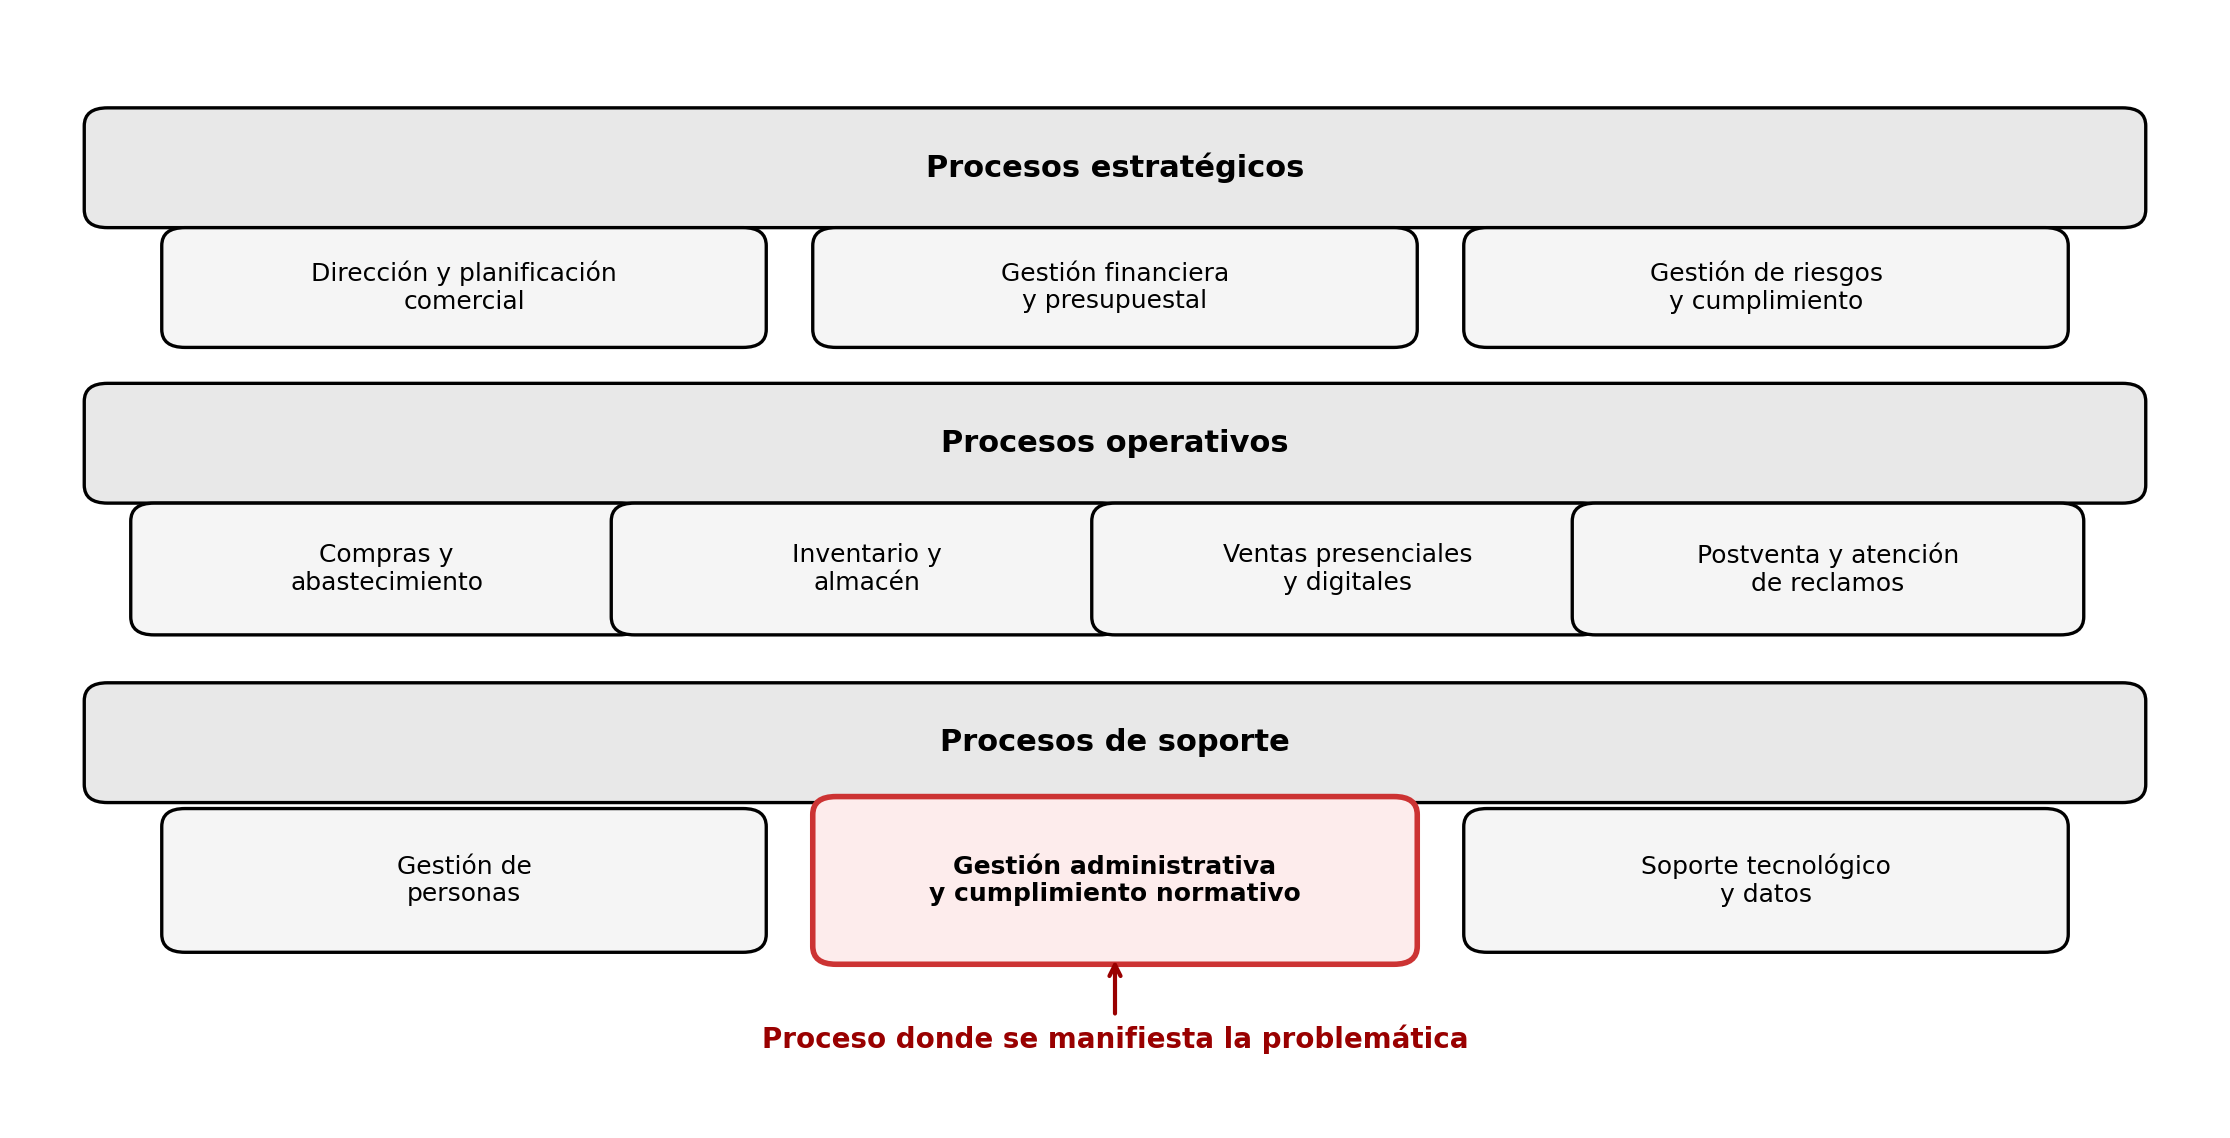
\includegraphics[width=0.98\textwidth]{figuras/mapa_procesos_pyme.png}
\figurenote{Elaboración propia.}
\end{figure}

\subsection{Campo de acción}\label{subsec:campo-de-accion}

El campo de acción corresponde al proceso de \textbf{gestión administrativa y cumplimiento normativo} de Comercial Andina Retail S.A.C. Este proceso comprende la identificación de normas aplicables, interpretación de obligaciones, asignación de responsables, registro de evidencias y seguimiento del cumplimiento ante entidades regulatorias. El alcance no incluye la emisión de asesoría legal vinculante, sino la generación de orientación operativa trazable para que la PYME pueda comprender qué debe revisar, qué acción debe ejecutar y qué fuente oficial sustenta la recomendación.

\textbf{Proceso AS-IS de cumplimiento normativo:}

\begin{enumerate}
\item La administradora o el contador externo revisa manualmente fuentes como SUNAT, SUNAFIL, INDECOPI, municipalidad, Diario Oficial \textit{El Peruano} y correos de notificación.
\item Se identifica si una norma, comunicado o requerimiento puede aplicar a la empresa según rubro, tamaño, número de trabajadores, ventas y canal de venta.
\item La información se interpreta manualmente y se consulta al contador o asesor externo cuando el lenguaje técnico no es claro.
\item Las tareas de cumplimiento se registran en hojas de cálculo, correos o mensajes de WhatsApp sin un repositorio único de trazabilidad.
\item La empresa ejecuta la acción correspondiente: declaración, pago, actualización documental, respuesta a requerimiento, corrección de comprobantes, actualización del Libro de Reclamaciones o revisión laboral.
\end{enumerate}

\textbf{Sistemas y fuentes involucradas:}

\begin{longtable}{@{}p{0.28\textwidth}p{0.36\textwidth}p{0.28\textwidth}@{}}
\caption{Sistemas y fuentes vinculadas al campo de acción}\label{tab:sistemas-fuentes-campo}\\
\toprule
\textbf{Sistema o fuente} & \textbf{Uso en la PYME} & \textbf{Limitación actual} \\
\midrule
\endfirsthead
\caption[]{Sistemas y fuentes vinculadas al campo de acción (continuación)}\\
\toprule
\textbf{Sistema o fuente} & \textbf{Uso en la PYME} & \textbf{Limitación actual} \\
\midrule
\endhead
Portal SUNAT / Clave SOL & Declaraciones, pagos, comprobantes electrónicos y comunicaciones tributarias. & Información dispersa entre módulos y comunicados. \\
T-Registro y PLAME & Gestión laboral tributaria y planilla electrónica. & Requiere interpretación de obligaciones laborales y tributarias. \\
SUNAFIL / Casilla electrónica & Notificaciones, inspecciones y orientación sociolaboral. & Seguimiento manual y riesgo de omitir plazos. \\
INDECOPI & Libro de Reclamaciones, protección al consumidor y publicidad comercial. & Normas aplicables difíciles de interpretar para personal no legal. \\
Municipalidad distrital & Licencia de funcionamiento, inspecciones técnicas y tributos municipales. & Requisitos locales no centralizados. \\
Diario Oficial \textit{El Peruano} & Fuente oficial de normas legales. & Alto volumen de documentos y lenguaje legal especializado. \\
Excel / Google Drive / WhatsApp & Registro interno de tareas y evidencias. & Baja trazabilidad, duplicidad de información y ausencia de alertas automáticas. \\
\bottomrule
\multicolumn{3}{p{0.94\textwidth}}{\normalsize \textit{Nota.} Elaboración propia.}\\
\end{longtable}

\subsection{Situación Problemática}\label{subsec:situacion-problematica}

La situación problemática se reformula a partir de un escenario de validación más coherente con la naturaleza de la solución SIR. El problema ya no se ubica en la entidad que publica normas, sino en la empresa que debe interpretarlas y aplicarlas. Comercial Andina Retail S.A.C. necesita cumplir obligaciones periódicas y eventuales, pero carece de un mecanismo centralizado para monitorear cambios regulatorios, interpretar su aplicabilidad y documentar las fuentes que sustentan cada decisión. Esta condición incrementa la carga operativa de la administración y genera dependencia del contador externo para consultas que podrían resolverse con una herramienta de apoyo interpretativo.

La pertinencia del problema también se relaciona con los mecanismos regulatorios vigentes. SUNAT reportó en su Informe de Gestión por Resultados 2024 una tasa de cumplimiento de presentación de declaraciones determinativas al vencimiento de 95.1\% y una tasa de morosidad global de 2.1\%, indicadores que muestran que el cumplimiento se gestiona con métricas observables \parencite{sunatGestion2024}. Además, SUNAT define el Perfil de Cumplimiento Tributario como una calificación orientada a incentivar el cumplimiento voluntario y establecer facilidades o limitaciones según el comportamiento del contribuyente \parencite{sunatPerfilCumplimiento2026}. Por ello, una PYME que no interpreta oportunamente sus obligaciones puede afectar su gestión tributaria, su nivel de riesgo y su relación con la administración pública.

\textbf{Proceso de recopilación de información para el diagnóstico}

Para construir una problemática medible, se plantea un diagnóstico inicial basado en tres técnicas: revisión documental de obligaciones aplicables a una PYME comercial, entrevista semiestructurada a tres roles clave y prueba cronometrada de interpretación normativa. Los roles considerados son: administrador general, contador externo y responsable de atención al cliente. La prueba consiste en entregar diez cambios o consultas normativas frecuentes y medir cuánto tarda el usuario en identificar la obligación, determinar si aplica a la empresa y registrar la fuente usada.

\begin{longtable}{@{}p{0.24\textwidth}p{0.32\textwidth}p{0.34\textwidth}@{}}
\caption{Matriz de diagnóstico inicial del proceso de cumplimiento}\label{tab:matriz-diagnostico}\\
\toprule
\textbf{Técnica} & \textbf{Aplicación} & \textbf{Resultado esperado para la línea base} \\
\midrule
\endfirsthead
\caption[]{Matriz de diagnóstico inicial del proceso de cumplimiento (continuación)}\\
\toprule
\textbf{Técnica} & \textbf{Aplicación} & \textbf{Resultado esperado para la línea base} \\
\midrule
\endhead
Revisión documental & Normas, comunicados, obligaciones SUNAT, obligaciones laborales, Libro de Reclamaciones y licencia municipal. & Lista de obligaciones recurrentes y eventuales aplicables a la PYME. \\
Entrevista semiestructurada & Administrador, contador externo y responsable de atención al cliente. & Identificación de causas operativas: dependencia externa, desconocimiento normativo y dispersión de fuentes. \\
Prueba cronometrada & Diez consultas normativas con medición de tiempo, exactitud y fuente citada. & Línea base de tiempo promedio, porcentaje de respuestas correctas y trazabilidad de fuentes. \\
\bottomrule
\multicolumn{3}{p{0.94\textwidth}}{\normalsize \textit{Nota.} Elaboración propia.}\\
\end{longtable}

A partir del diagnóstico inicial, se establece la siguiente línea base preliminar para validar posteriormente el impacto del SIR:

\begin{longtable}{@{}p{0.38\textwidth}p{0.22\textwidth}p{0.30\textwidth}@{}}
\caption{Línea base de la problemática}\label{tab:linea-base-problematica}\\
\toprule
\textbf{Indicador de línea base} & \textbf{Valor inicial} & \textbf{Evidencia de medición} \\
\midrule
\endfirsthead
\caption[]{Línea base de la problemática (continuación)}\\
\toprule
\textbf{Indicador de línea base} & \textbf{Valor inicial} & \textbf{Evidencia de medición} \\
\midrule
\endhead
Tiempo promedio para interpretar una consulta normativa y decidir aplicabilidad. & 90 minutos por consulta. & Prueba cronometrada con diez casos de consulta. \\
Exactitud en la identificación de obligaciones aplicables sin apoyo externo. & 55\%. & Comparación con matriz de respuesta esperada revisada por contador. \\
Consultas que requieren intervención del contador o asesor externo. & 70\%. & Registro de consultas derivadas durante la prueba. \\
Respuestas con fuente oficial claramente registrada. & 30\%. & Revisión de evidencias y enlaces citados por el usuario. \\
Tiempo semanal dedicado a revisión normativa y coordinación de cumplimiento. & 5 horas por semana. & Estimación de entrevista y bitácora administrativa. \\
Costo mensual aproximado de consultas externas adicionales. & S/ 600. & Estimación de asesoría contable/legal registrada para el diagnóstico inicial. \\
\bottomrule
\multicolumn{3}{p{0.94\textwidth}}{\normalsize \textit{Nota.} Valores de línea base preliminar; deberán contrastarse con usuarios durante la ejecución del proyecto.}\\
\end{longtable}

\textbf{Problema central reformulado}

La PYME comercial presenta una \textbf{baja eficiencia y trazabilidad en la interpretación de obligaciones normativas aplicables}, debido a la dispersión de fuentes regulatorias, el lenguaje técnico-legal, la ausencia de monitoreo automatizado y el uso de controles manuales. Esta situación genera demoras en la toma de decisiones de cumplimiento, dependencia de asesoría externa, riesgo de omisión de obligaciones y dificultad para demostrar qué fuente sustentó una acción administrativa.

\textbf{Análisis del problema mediante Árbol de Problemas}

El Árbol de Problemas de la Figura~\ref{fig:arbol-problemas-pyme} organiza la problemática en tres niveles: causas, problema central y efectos. Las causas se agrupan en información dispersa, limitaciones internas de conocimiento, ausencia de automatización y controles manuales. El problema central se expresa en términos medibles: baja eficiencia y baja trazabilidad en la interpretación normativa. Los efectos se relacionan con retrasos operativos, mayor costo de asesoría, riesgo de incumplimiento y baja capacidad de seguimiento.

\begin{figure}[H]
\centering
\caption{Árbol de problemas reformulado para la PYME comercial}
\label{fig:arbol-problemas-pyme}
\vspace{0.35em}
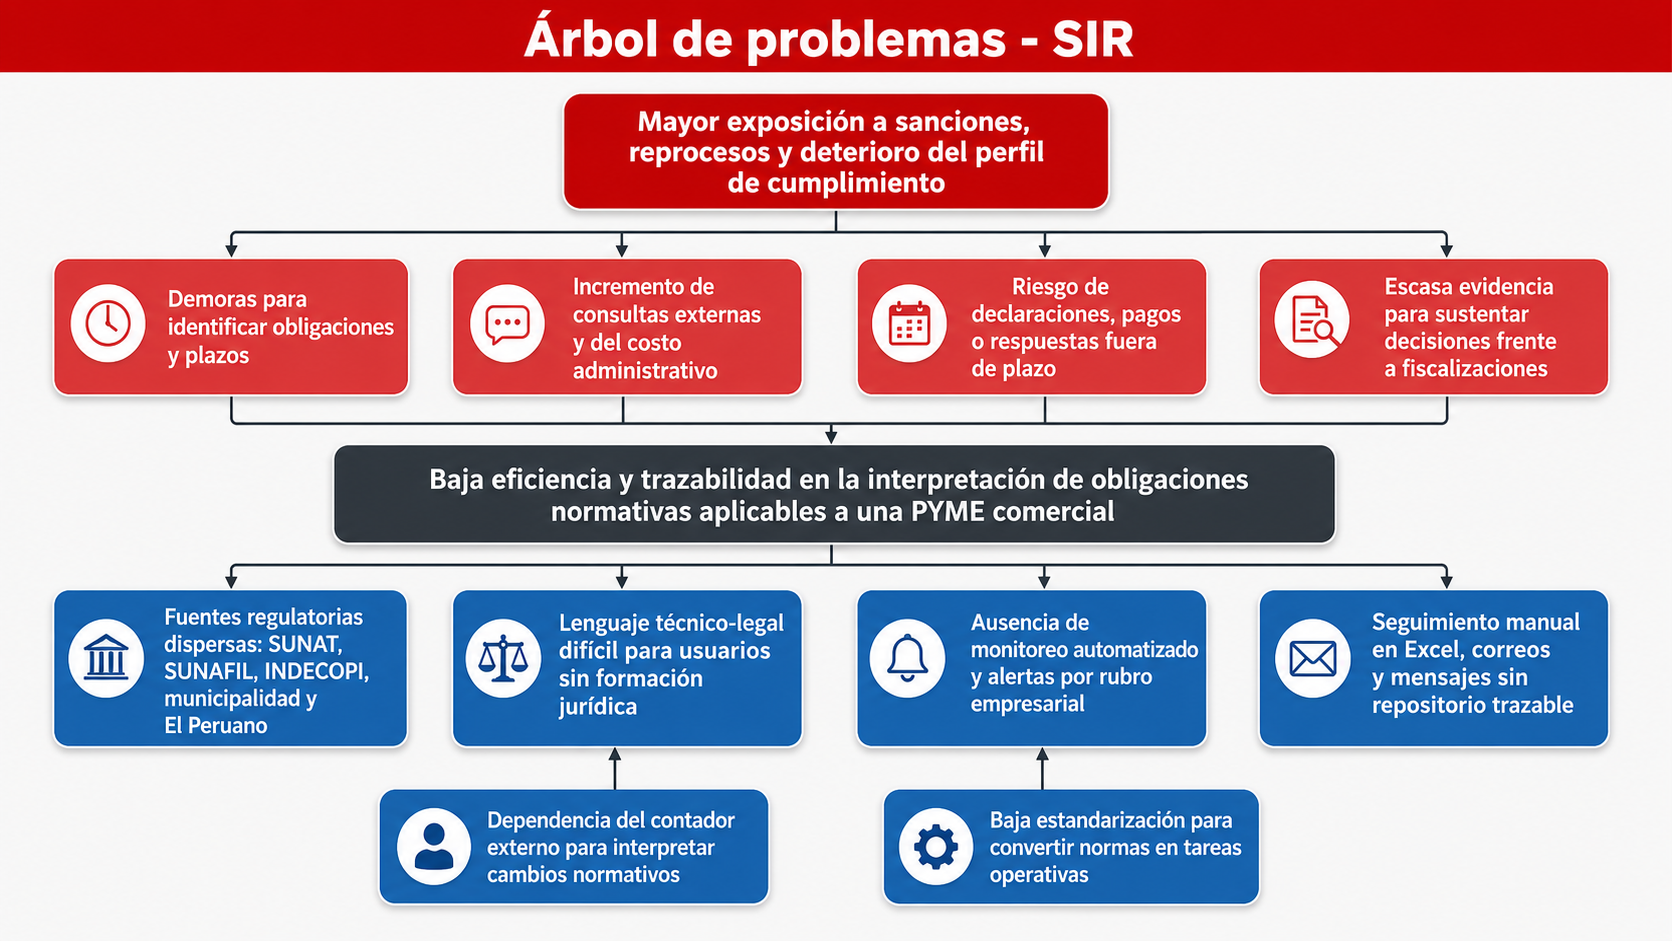
\includegraphics[width=0.98\textwidth]{figuras/arbol_problemas_pyme.png}
\figurenote{Elaboración propia.}
\end{figure}

\textbf{Análisis del problema mediante Diagrama de Ishikawa}

El Diagrama de Ishikawa de la Figura~\ref{fig:ishikawa-pyme} complementa el Árbol de Problemas al clasificar las causas en seis dimensiones: personas, métodos, tecnología, información, normativa y gestión. Esta lectura permite distinguir causas técnicas y causas de negocio, lo cual facilita formular objetivos e indicadores de éxito coherentes con la solución SIR.

\begin{figure}[H]
\centering
\caption{Diagrama de Ishikawa reformulado para la problemática de cumplimiento}
\label{fig:ishikawa-pyme}
\vspace{0.35em}
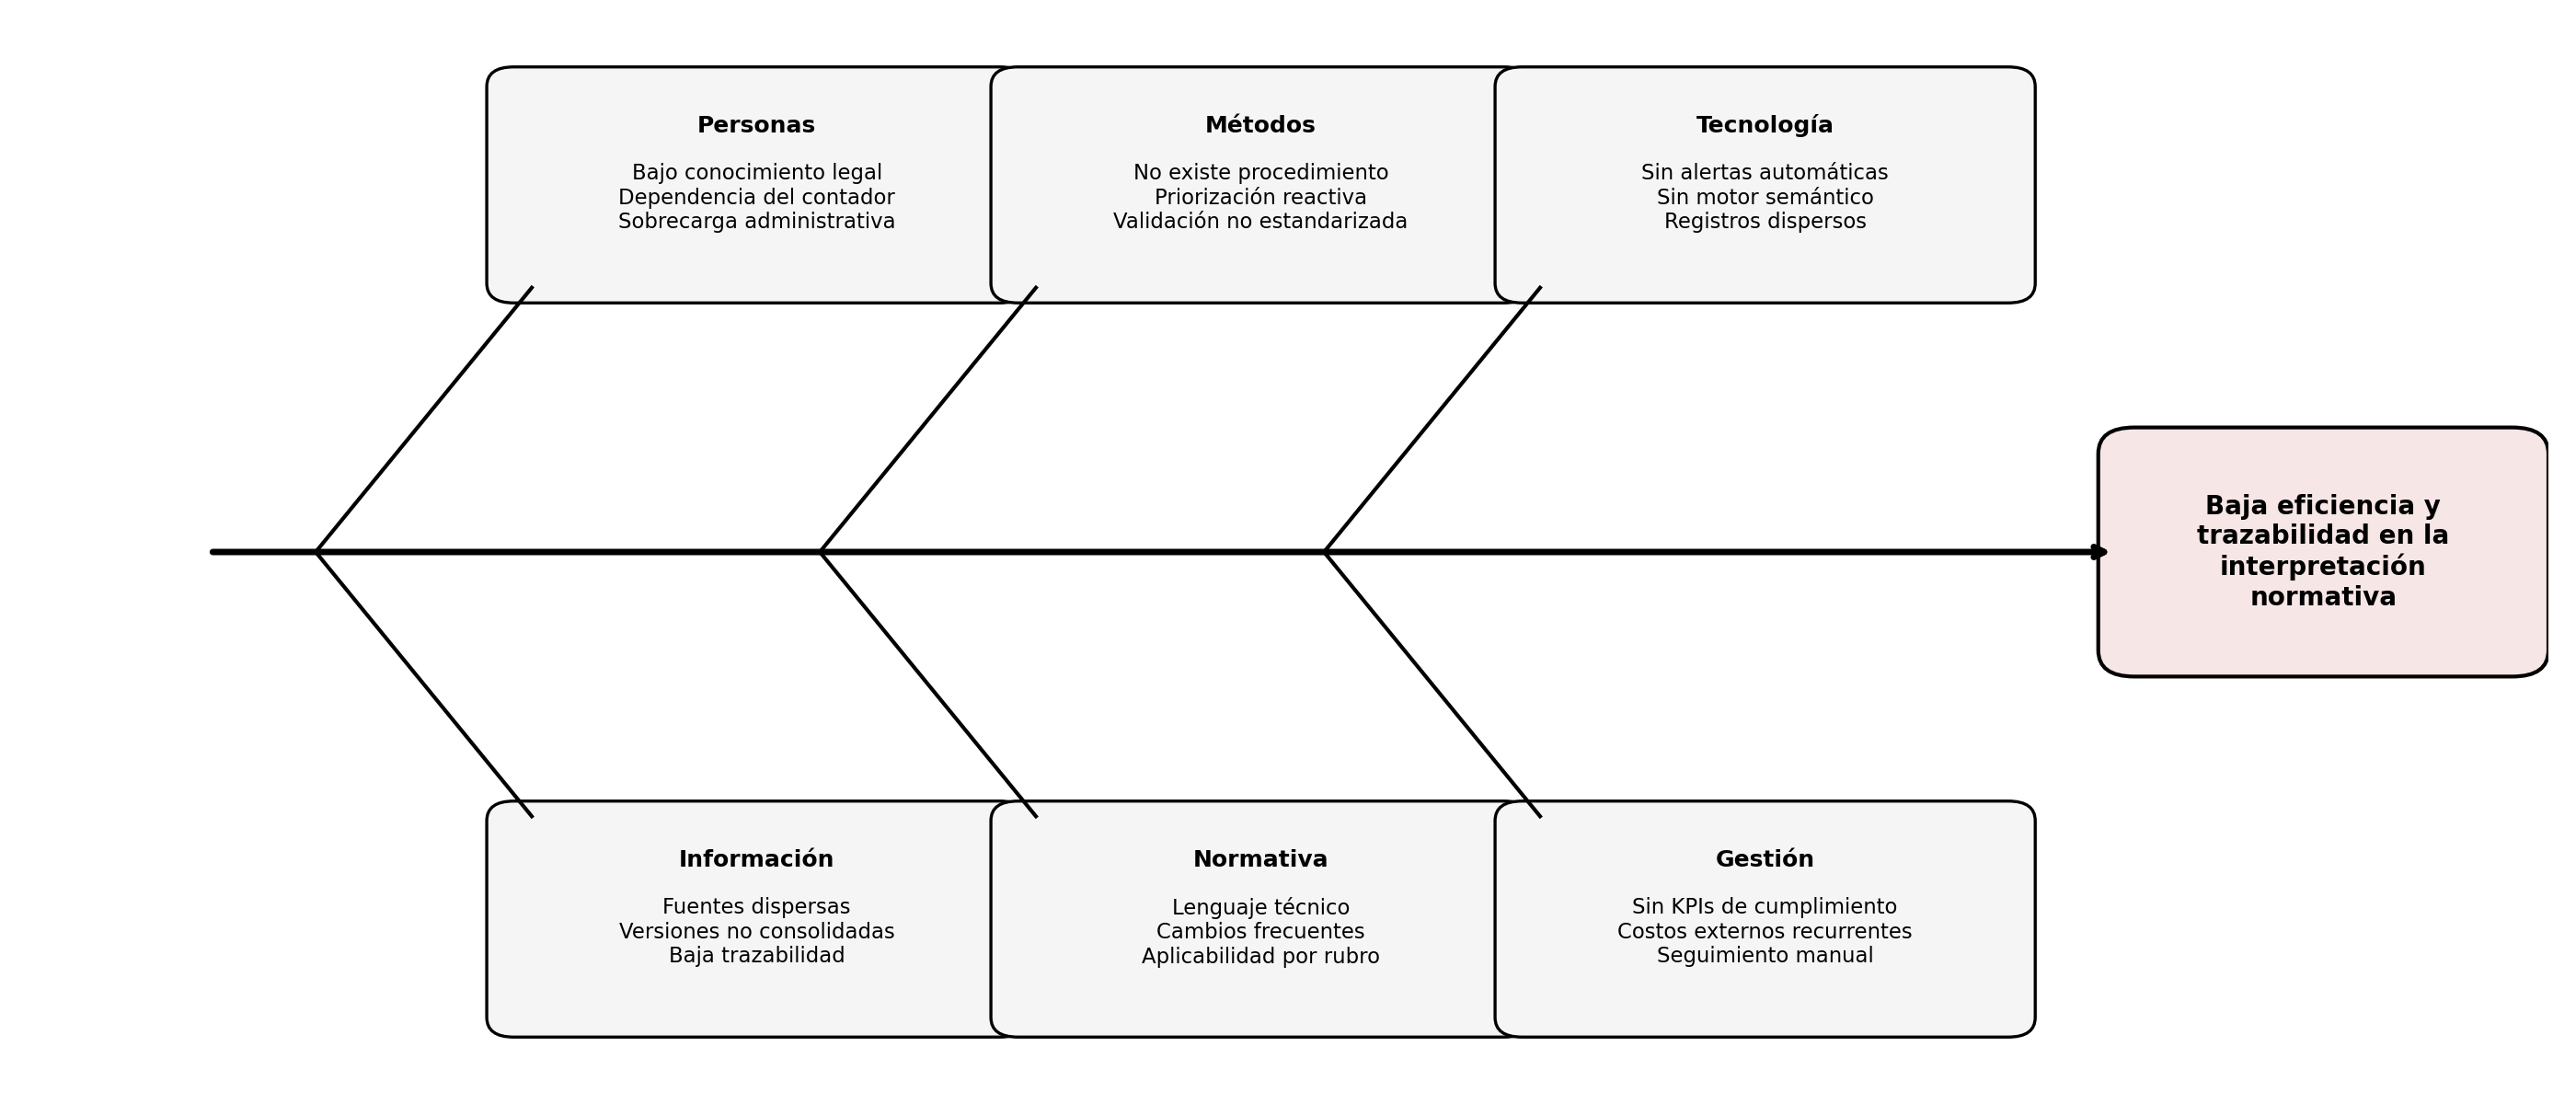
\includegraphics[width=0.98\textwidth]{figuras/ishikawa_pyme.png}
\figurenote{Elaboración propia.}
\end{figure}

\subsection{Problemas a resolver}\label{subsec:problemas-a-resolver}

A partir del diagnóstico, los problemas a resolver se estructuran en dimensiones técnicas y de negocio. Esta organización evita que la problemática quede formulada de manera general y permite vincular cada causa con una capacidad esperada del SIR. La Tabla~\ref{tab:problemas-resolver} sintetiza el problema central, sus causas principales y el enfoque de atención propuesto.

\begin{longtable}{@{}p{0.20\textwidth}p{0.36\textwidth}p{0.34\textwidth}@{}}
\caption{Problemas a resolver según dimensión}\label{tab:problemas-resolver}\\
\toprule
\textbf{Dimensión} & \textbf{Descripción del problema} & \textbf{Orientación de solución} \\
\midrule
\endfirsthead
\caption[]{Problemas a resolver según dimensión (continuación)}\\
\toprule
\textbf{Dimensión} & \textbf{Descripción del problema} & \textbf{Orientación de solución} \\
\midrule
\endhead
Problema central & Baja eficiencia y trazabilidad en la interpretación de obligaciones normativas aplicables a una PYME comercial. & Implementar un asistente de inteligencia regulatoria que responda consultas con fuentes oficiales y orientación operativa. \\
Causas técnicas & Ausencia de monitoreo automatizado, búsqueda semántica, repositorio centralizado y capa de citación verificable. & Diseñar arquitectura RAG con ingesta normativa, recuperación vectorial, generación controlada y citación de fuentes. \\
Causas de negocio & Dependencia del contador externo, desconocimiento del lenguaje legal, seguimiento manual de plazos y poca claridad sobre aplicabilidad por rubro. & Configurar perfil empresarial, alertas y respuestas adaptadas al tamaño, rubro y obligaciones de la PYME. \\
Impactos medibles & Tiempo alto de interpretación, baja exactitud, bajo registro de fuentes y costos recurrentes de asesoría. & Validar reducción de tiempo, mejora de exactitud, cobertura de citaciones y satisfacción del usuario. \\
\bottomrule
\multicolumn{3}{p{0.94\textwidth}}{\normalsize \textit{Nota.} Elaboración propia.}\\
\end{longtable}

\textbf{Formulación del problema general}

¿De qué manera la implementación de un Sistema de Inteligencia Regulatoria basado en IA generativa y arquitectura RAG puede reducir el tiempo de interpretación normativa y mejorar la trazabilidad de fuentes en el proceso de cumplimiento de una PYME comercial peruana?

\textbf{Problemas específicos}

\begin{itemize}
\item La PYME no cuenta con un proceso centralizado para monitorear cambios normativos aplicables a su rubro, tamaño y ubicación.
\item La interpretación de normas tributarias, laborales y comerciales depende de personal sin formación jurídica o del contador externo.
\item Las fuentes oficiales usadas para tomar decisiones de cumplimiento no se registran de manera uniforme ni trazable.
\item Los plazos y acciones derivadas de cambios normativos se controlan manualmente, lo que genera riesgo de omisión o demora.
\item No existen indicadores internos para medir tiempo de interpretación, exactitud, cobertura de fuentes y satisfacción del usuario en el proceso de cumplimiento.
\end{itemize}

\section{Definición de la Solución}\label{sec:definicion-de-la-solucion}

La solución propuesta es el Sistema de Inteligencia Regulatoria (SIR), una plataforma web de apoyo al cumplimiento normativo para PYMEs comerciales. El sistema integrará un perfil empresarial, un motor de recuperación de normas oficiales, un asistente conversacional basado en IA generativa y una capa de citación que permita verificar la procedencia de cada respuesta. La solución no reemplaza al contador ni al asesor legal; su función es reducir la carga operativa de búsqueda e interpretación preliminar, transformando normas complejas en respuestas accionables, trazables y contextualizadas.

\subsection{Objetivos del Proyecto}\label{subsec:objetivos-del-proyecto}

\textbf{Objetivo General}

Implementar un Sistema de Inteligencia Regulatoria basado en IA generativa y arquitectura RAG para automatizar la interpretación preliminar de obligaciones normativas aplicables a una PYME comercial peruana, con el fin de reducir al menos en 60\% el tiempo promedio de comprensión normativa y alcanzar una cobertura de citaciones oficiales de al menos 95\% durante la validación del prototipo.

\textbf{Objetivos Específicos}

\begin{itemize}
\item \textbf{OE1:} Diagnosticar el proceso actual de identificación e interpretación normativa de la PYME comercial, estableciendo una línea base de tiempo, exactitud, dependencia externa y trazabilidad de fuentes.
\item \textbf{OE2:} Diseñar la arquitectura lógica y funcional del SIR mediante un enfoque RAG que integre ingesta normativa, almacenamiento vectorial, recuperación semántica, generación de respuestas y citación verificable.
\item \textbf{OE3:} Desarrollar un prototipo funcional del SIR que permita registrar el perfil empresarial, realizar consultas en lenguaje natural, generar respuestas contextualizadas y mostrar fuentes oficiales vinculadas.
\item \textbf{OE4:} Validar el desempeño técnico, operativo y de usabilidad del prototipo mediante métricas de precisión, tiempo de respuesta, reducción del tiempo de interpretación, cobertura de citaciones y satisfacción del usuario.
\end{itemize}

\subsection{Indicadores de Éxito}\label{subsec:indicadores-de-exito}

Los indicadores de éxito se reformulan para asegurar correspondencia directa con los objetivos específicos y con la problemática medible del Capítulo 1. Cada indicador incluye fórmula, tipo de ratio, umbral de aceptación y objetivo asociado.

\begin{longtable}{@{}p{0.09\textwidth}p{0.25\textwidth}p{0.28\textwidth}p{0.13\textwidth}p{0.12\textwidth}p{0.07\textwidth}@{}}
\caption{Indicadores de éxito del proyecto}\label{tab:indicadores-exito-reformulados}\\
\toprule
\textbf{Código} & \textbf{Descripción} & \textbf{Fórmula} & \textbf{Ratio} & \textbf{Umbral} & \textbf{Objetivo} \\
\midrule
\endfirsthead
\caption[]{Indicadores de éxito del proyecto (continuación)}\\
\toprule
\textbf{Código} & \textbf{Descripción} & \textbf{Fórmula} & \textbf{Ratio} & \textbf{Umbral} & \textbf{Objetivo} \\
\midrule
\endhead
IE1 & Línea base documentada del proceso AS-IS. & Casos diagnosticados / casos planificados. & Porcentaje & 100\% & OE1 \\
IE2 & Reducción del tiempo de interpretación normativa. & (Tiempo base - tiempo con SIR) / tiempo base. & Porcentaje & $\geq$ 60\% & OE4 \\
IE3 & Precisión de recuperación e interpretación. & F1-Score sobre dataset etiquetado. & Índice & $\geq$ 0.85 & OE4 \\
IE4 & Cobertura de citaciones oficiales. & Respuestas con fuente oficial / total de respuestas. & Porcentaje & $\geq$ 95\% & OE2/OE4 \\
IE5 & Tiempo promedio de respuesta del chatbot. & Suma de tiempos de respuesta / total de consultas. & Segundos & $<$ 8 s & OE3/OE4 \\
IE6 & Usabilidad percibida. & Puntuación System Usability Scale. & Puntaje & $\geq$ 75 & OE4 \\
IE7 & Contextualización por perfil empresarial. & Respuestas que consideran rubro/tamaño / total de respuestas aplicables. & Porcentaje & $\geq$ 90\% & OE3 \\
IE8 & Disponibilidad del prototipo en ambiente de validación. & Tiempo operativo / tiempo total planificado. & Porcentaje & $\geq$ 99\% & OE3 \\
\bottomrule
\multicolumn{6}{p{0.94\textwidth}}{\normalsize \textit{Nota.} Elaboración propia.}\\
\end{longtable}

\subsection{Factibilidad del Proyecto}\label{subsec:factibilidad-del-proyecto}

La factibilidad del proyecto se analiza considerando las dimensiones económica y técnica, debido a que el prototipo debe ser implementado, desplegado y validado con usuarios finales en un ambiente controlado. Este análisis permite determinar si la solución puede ejecutarse con los recursos disponibles, qué dificultades podrían presentarse y bajo qué condiciones puede operar de manera sostenible. En esa línea, la evaluación económica se orienta a la relación costo-beneficio, mientras que la evaluación técnica revisa si existen conocimientos, herramientas e infraestructura suficientes para desarrollar la solución.

\subsubsection{Factibilidad Económica}\label{subsubsec:factibilidad-economica}

La factibilidad económica estima los costos necesarios para construir, desplegar y validar el SIR en Comercial Andina Retail S.A.C. Este análisis permite evaluar si conviene ejecutar el proyecto a partir de criterios cuantitativos y cualitativos como VAN, TIR, periodo de recuperación y relación costo-beneficio. Para este proyecto, los costos se dividen en recursos humanos, infraestructura cloud, software/licencias, hardware y otros gastos operativos.

\textbf{Mapeo de costos involucrados}

\begin{longtable}{@{}p{0.24\textwidth}p{0.46\textwidth}p{0.20\textwidth}@{}}
\caption{Mapeo de costos de inversión inicial}\label{tab:mapeo-costos}\\
\toprule
\textbf{Tipo} & \textbf{Detalle} & \textbf{Costo estimado} \\
\midrule
\endfirsthead
\caption[]{Mapeo de costos de inversión inicial (continuación)}\\
\toprule
\textbf{Tipo} & \textbf{Detalle} & \textbf{Costo estimado} \\
\midrule
\endhead
Recursos humanos & Análisis, diseño, desarrollo, pruebas y documentación del prototipo por dos integrantes del equipo. & S/ 18,000 \\
Infraestructura & Ambiente cloud para API, base de datos, almacenamiento y pruebas de despliegue. & S/ 2,400 \\
Software/licencias & Consumo inicial de API de IA, herramientas de desarrollo, monitoreo y servicios de integración. & S/ 3,600 \\
Hardware & Uso de laptops del equipo y dispositivos de prueba. No se requiere adquisición adicional. & S/ 0 \\
Otros & Validación con usuarios, documentación, contingencia y materiales administrativos. & S/ 2,850 \\
\textbf{Total inversión inicial} & & \textbf{S/ 26,850} \\
\bottomrule
\multicolumn{3}{p{0.94\textwidth}}{\normalsize \textit{Nota.} Elaboración propia con valores estimados para el escenario de validación.}\\
\end{longtable}

\textbf{Beneficios esperados}

Los beneficios económicos esperados provienen principalmente de la reducción de horas administrativas dedicadas a búsqueda normativa, disminución de consultas externas recurrentes, reducción de reprocesos y mejora en la oportunidad de cumplimiento. La Tabla~\ref{tab:beneficios-esperados} presenta una estimación anual conservadora.

\begin{longtable}{@{}p{0.42\textwidth}p{0.30\textwidth}p{0.18\textwidth}@{}}
\caption{Beneficios económicos esperados}\label{tab:beneficios-esperados}\\
\toprule
\textbf{Beneficio} & \textbf{Supuesto de cálculo} & \textbf{Ahorro anual} \\
\midrule
\endfirsthead
\caption[]{Beneficios económicos esperados (continuación)}\\
\toprule
\textbf{Beneficio} & \textbf{Supuesto de cálculo} & \textbf{Ahorro anual} \\
\midrule
\endhead
Reducción de horas administrativas & Ahorro de 3 horas semanales a S/ 35 por hora durante 48 semanas. & S/ 5,040 \\
Reducción de consultas externas & Disminución de S/ 600 a S/ 250 mensuales en consultas adicionales. & S/ 4,200 \\
Menor reproceso documental & Reducción de correcciones, búsqueda de fuentes y duplicidad documental. & S/ 3,480 \\
Prevención de contingencias menores & Menor exposición a pagos por errores operativos y retrasos menores. & S/ 6,000 \\
\textbf{Total beneficio anual estimado} & & \textbf{S/ 18,720} \\
\bottomrule
\multicolumn{3}{p{0.94\textwidth}}{\normalsize \textit{Nota.} Elaboración propia con valores s para fines de evaluación económica preliminar.}\\
\end{longtable}

\textbf{Análisis financiero}

Se proyecta un flujo de caja a tres años con una inversión inicial de S/ 26,850, beneficios crecientes por adopción progresiva y costos operativos anuales asociados al uso de servicios cloud, API de IA y mantenimiento del prototipo. Se utiliza una tasa de descuento referencial de 12\%.

\begin{longtable}{@{}p{0.20\textwidth}p{0.20\textwidth}p{0.20\textwidth}p{0.20\textwidth}@{}}
\caption{Flujo de caja proyectado a tres años}\label{tab:flujo-caja}\\
\toprule
\textbf{Periodo} & \textbf{Beneficios} & \textbf{Costos operativos} & \textbf{Flujo neto} \\
\midrule
\endfirsthead
\caption[]{Flujo de caja proyectado a tres años (continuación)}\\
\toprule
\textbf{Periodo} & \textbf{Beneficios} & \textbf{Costos operativos} & \textbf{Flujo neto} \\
\midrule
\endhead
Año 0 & S/ 0 & S/ 26,850 & -S/ 26,850 \\
Año 1 & S/ 18,720 & S/ 5,240 & S/ 13,480 \\
Año 2 & S/ 20,030 & S/ 5,502 & S/ 14,528 \\
Año 3 & S/ 21,432 & S/ 5,777 & S/ 15,655 \\
\bottomrule
\multicolumn{4}{p{0.94\textwidth}}{\normalsize \textit{Nota.} Elaboración propia.}\\
\end{longtable}

\begin{longtable}{@{}p{0.28\textwidth}p{0.26\textwidth}p{0.36\textwidth}@{}}
\caption{Indicadores financieros preliminares}\label{tab:indicadores-financieros}\\
\toprule
\textbf{Indicador} & \textbf{Resultado} & \textbf{Interpretación} \\
\midrule
\endfirsthead
\caption[]{Indicadores financieros preliminares (continuación)}\\
\toprule
\textbf{Indicador} & \textbf{Resultado} & \textbf{Interpretación} \\
\midrule
\endhead
Valor Actual Neto (VAN) & S/ 7,910 & Al ser positivo, indica que el proyecto genera valor bajo los supuestos estimados. \\
Tasa Interna de Retorno (TIR) & 28.0\% & Supera la tasa de descuento referencial de 12\%, por lo que el proyecto es atractivo. \\
Periodo de recuperación & Entre el año 2 y 3 & La inversión se recupera dentro del horizonte de evaluación. \\
Relación beneficio/costo & 1.29 & Por cada sol invertido se obtiene un retorno estimado de S/ 1.29. \\
\bottomrule
\multicolumn{3}{p{0.94\textwidth}}{\normalsize \textit{Nota.} Cálculo preliminar con tasa de descuento de 12\%.}\\
\end{longtable}

Con base en los resultados, el proyecto es económicamente viable para Comercial Andina Retail S.A.C. en una etapa inicial de validación controlada. El VAN positivo, la TIR superior a la tasa de descuento y la recuperación dentro del horizonte de tres años indican que la inversión estimada se justifica por la reducción de carga administrativa, consultas externas y reprocesos asociados al cumplimiento normativo.

\subsubsection{Factibilidad Técnica}\label{subsubsec:factibilidad-tecnica}

La factibilidad técnica evalúa si el equipo dispone de conocimientos, herramientas, infraestructura y metodología suficientes para construir el SIR. En este caso, la solución es técnicamente viable porque se basa en tecnologías maduras y ampliamente documentadas: Python, FastAPI, React, LangChain, modelos de lenguaje, embeddings y bases vectoriales.

\begin{longtable}{@{}p{0.28\textwidth}p{0.62\textwidth}@{}}
\caption{Evaluación de factibilidad técnica}\label{tab:factibilidad-tecnica}\\
\toprule
\textbf{Tipo} & \textbf{Detalles} \\
\midrule
\endfirsthead
\caption[]{Evaluación de factibilidad técnica (continuación)}\\
\toprule
\textbf{Tipo} & \textbf{Detalles} \\
\midrule
\endhead
Infraestructura disponible & Despliegue cloud ligero para API, base de datos relacional, almacenamiento documental y base vectorial. Se priorizan servicios serverless o free-tier durante la validación. \\
Software y herramientas & Python, FastAPI, React, TypeScript, LangChain, OpenAI API, Pinecone o Qdrant, PostgreSQL, GitHub, Docker y herramientas de monitoreo básico. \\
Metodología tecnológica & Arquitectura RAG con ingesta, limpieza, segmentación, embeddings, recuperación Top-K, generación controlada y capa de citación. Desarrollo iterativo bajo Scrum. \\
Alternativas evaluadas & Pinecone frente a Qdrant para base vectorial; OpenAI frente a modelos open-source; Vercel frente a despliegue cloud tradicional. Se prioriza menor complejidad operativa. \\
Riesgos y limitaciones técnicas & Dependencia de API externa, costos variables por consumo, límites de contexto del modelo, necesidad de curar fuentes oficiales y riesgo de alucinaciones mitigado mediante citaciones y respuestas con disclaimer. \\
\bottomrule
\multicolumn{2}{p{0.94\textwidth}}{\normalsize \textit{Nota.} Elaboración propia.}\\
\end{longtable}

El proyecto es técnicamente viable porque el equipo cuenta con conocimientos de desarrollo web, Python, integración de APIs, bases de datos y arquitectura de software. Asimismo, el alcance se limita a un prototipo validable en Comercial Andina Retail S.A.C., lo que reduce la complejidad de despliegue y permite concentrar la evaluación en la reducción de tiempo, trazabilidad y usabilidad.

\subsection{Propuesta preliminar de la solución}\label{subsec:propuesta-preliminar-solucion}

La propuesta preliminar del SIR se plantea como un proceso TO-BE de apoyo al cumplimiento normativo. En lugar de que la PYME revise manualmente múltiples portales y dependa del contador externo para interpretar cada cambio, el sistema centraliza la consulta normativa, recupera fuentes oficiales, genera una respuesta operativa y muestra la evidencia que sustenta la recomendación. Esta propuesta mantiene al usuario humano como responsable de la decisión final y al contador o asesor como validador en casos de alta complejidad.

\textbf{Alcance funcional de alto nivel}

\begin{itemize}
\item Registro del perfil empresarial: rubro, tamaño, ubicación, régimen tributario, número de trabajadores y canales de venta.
\item Ingesta y consulta de normas oficiales provenientes del Diario Oficial \textit{El Peruano} y entidades regulatorias relevantes.
\item Chatbot de consultas en lenguaje natural para preguntas tributarias, laborales, municipales y de protección al consumidor.
\item Respuestas contextualizadas según perfil de la PYME, con resumen operativo, nivel de aplicabilidad y fuente oficial citada.
\item Alertas de cambios normativos relevantes y recordatorios de obligaciones recurrentes.
\item Exportación de respuestas y evidencias para revisión del contador o asesor externo.
\end{itemize}

\textbf{Proceso TO-BE propuesto}

La Figura~\ref{fig:to-be-sir} presenta el flujo conceptual de la solución propuesta. Este flujo no representa aún la arquitectura técnica detallada, sino la manera en que el SIR apoyará el proceso de negocio de la PYME.

\begin{figure}[H]
\centering
\caption{Proceso TO-BE de cumplimiento normativo asistido por SIR}
\label{fig:to-be-sir}
\vspace{0.35em}
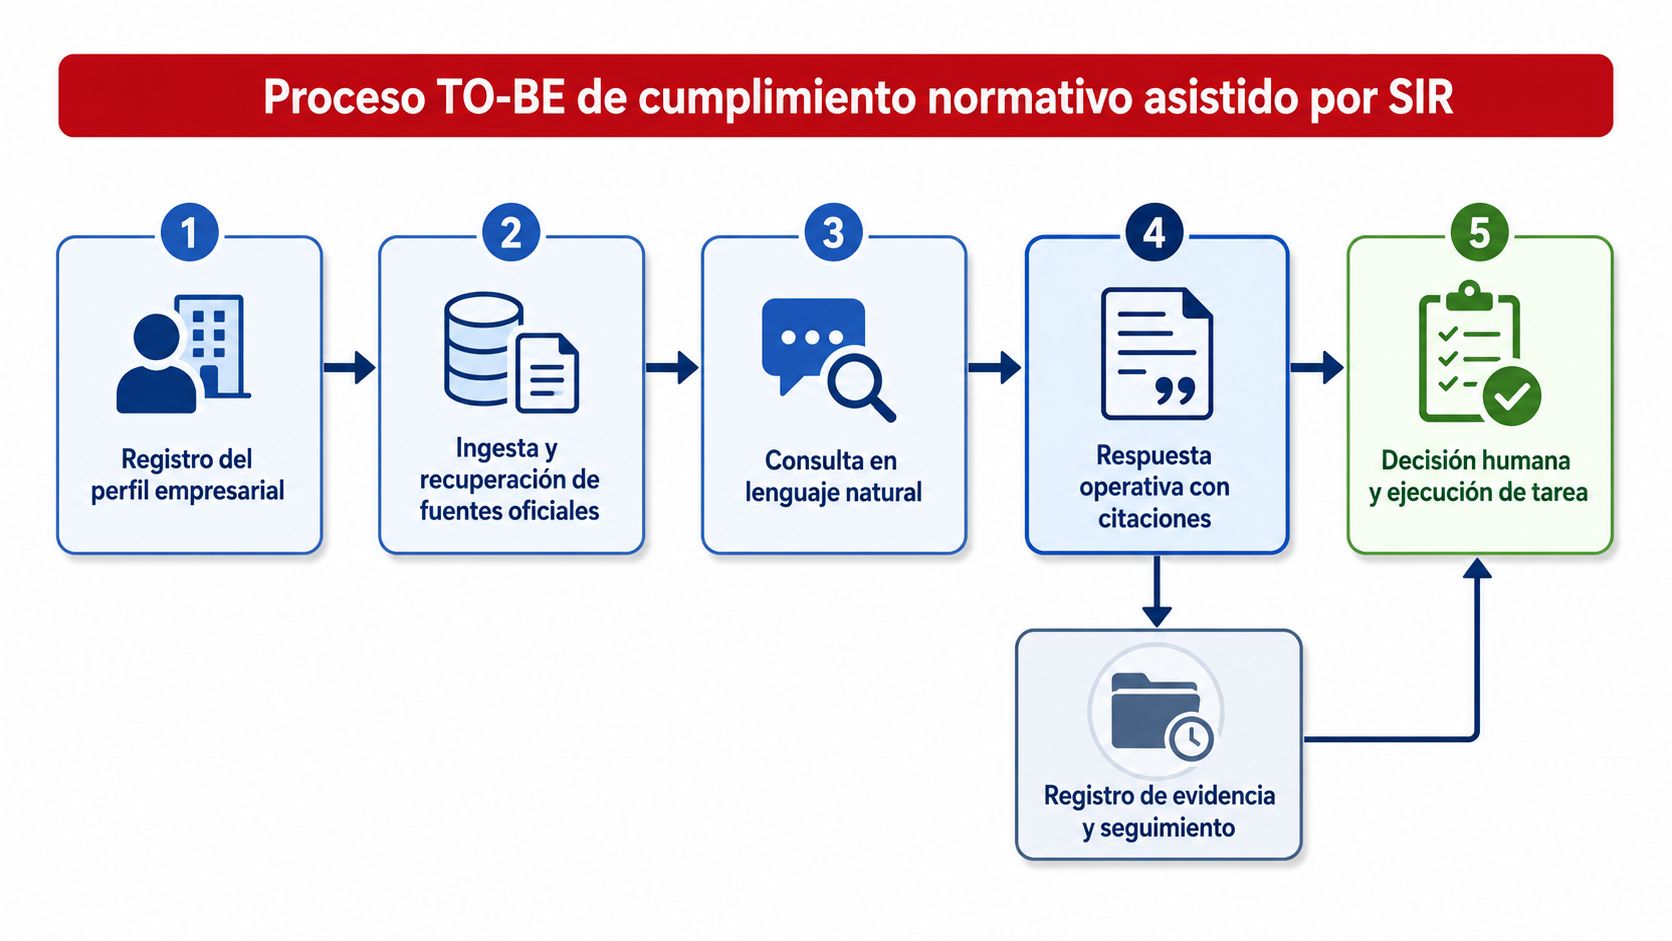
\includegraphics[width=0.98\textwidth]{figuras/to_be_sir.png}
\figurenote{Elaboración propia.}
\end{figure}

En síntesis, el Capítulo 1 define un escenario medible y validable: Comercial Andina Retail S.A.C., una PYME comercial que necesita reducir la carga de interpretación normativa. Esta definición mejora la coherencia entre problemática, objeto de estudio, indicadores, factibilidad y solución propuesta, y permite que los capítulos siguientes desarrollen la arquitectura, implementación y validación del SIR con mayor precisión.

\chapter{Marco Teórico}\label{cap:2-marco-teorico}

El presente capítulo desarrolla los fundamentos teóricos que sustentan la propuesta de solución basada en Inteligencia Artificial Generativa con arquitectura \textit{Retrieval-Augmented Generation} (RAG), aplicada a la interpretación de normas legales para una PYME comercial peruana. A partir de la revisión sistemática de literatura especializada y de marcos conceptuales actualizados, se establecen las bases académicas, técnicas y normativas que permiten comprender la problemática del cumplimiento normativo en las PYMEs y orientar el diseño del sistema propuesto.

El capítulo se organiza en tres dimensiones complementarias. En la primera parte, se presenta el marco teórico relacionado al negocio y a los procesos, donde se describen los conceptos, modelos y prácticas vinculadas con el cumplimiento normativo, la gestión de riesgo regulatorio (GRC) y la transformación digital del Estado peruano. En la segunda parte, se aborda el marco teórico de las tecnologías de información, que incluye los fundamentos de Procesamiento de Lenguaje Natural, modelos de lenguaje grandes (LLMs), arquitectura RAG y métricas estándar para evaluar sistemas de IA en dominios legales. Finalmente, se expone el marco de cumplimiento normativo, destacando las leyes peruanas y los estándares internacionales que orientan el diseño y operación de soluciones RegTech responsables.

Este capítulo resulta esencial porque proporciona el sustento científico y técnico que respalda la coherencia entre los objetivos del proyecto, la solución propuesta y las metodologías adoptadas. Los hallazgos se apoyan en una revisión sistemática de 24 artículos científicos indexados en bases académicas como Scopus, IEEE Xplore, ACM Digital Library y SpringerLink, con énfasis en los aportes de \textcite{singh2022}, \textcite{raju2025} y \textcite{noronha2025} como fuentes principales que sustentan el enfoque conceptual, técnico y de validación del Sistema de Inteligencia Regulatoria (SIR).

\section{Marco teórico relacionado al negocio y a los procesos}\label{sec:marco-teorico-negocio-procesos}

La presente sección desarrolla los fundamentos conceptuales vinculados con la operación y gestión del cumplimiento normativo en organizaciones empresariales, con énfasis en el segmento PYME. Se abordan cinco bloques temáticos: la definición y evolución del campo RegTech y SupTech; el modelo Governance, Risk and Compliance (GRC) como articulador del cumplimiento; la caracterización del segmento PYME peruano; los procesos administrativos de cumplimiento tributario, laboral y sectorial; y las experiencias internacionales de innovación regulatoria que sirven de referencia.

\subsection{RegTech y SupTech: definición y evolución}\label{subsec:regtech-suptech-definicion-evolucion}

El término RegTech, acuñado por la Financial Conduct Authority del Reino Unido en 2015, designa al conjunto de tecnologías de información, datos, inteligencia artificial y software utilizadas por las organizaciones para cumplir con regulaciones de manera más eficaz y eficiente \parencite{elkhoury2025}. Complementariamente, SupTech (\textit{Supervisory Technology}) describe el uso de tecnología por parte de las autoridades regulatorias para la supervisión y aplicación de las normas, con casos de uso que incluyen el seguimiento automatizado de cambios normativos, el \textit{reporting} estandarizado y la detección de fraude \parencite{chao2022}.

Desde su origen en el sector financiero, el campo RegTech ha experimentado una expansión hacia otras industrias reguladas, incluyendo el sector legal (LegalTech), el sector salud (HealthTech regulatorio) y el tercer sector (CharityTech). \textcite{singh2022} demuestran que las tecnologías de aprendizaje automático aplicadas al cumplimiento normativo pueden transferirse de organizaciones financieras a organizaciones con recursos limitados, como las entidades benéficas en el Reino Unido, donde los autores proponen un \enquote{Machine-Executable Compliance Toolkit} capaz de actualizar políticas internas y generar alertas de manera autónoma frente a cambios normativos. Este marco conceptual constituye una base teórica del presente proyecto, pues evidencia que la automatización del cumplimiento no se limita a grandes corporaciones y resulta aplicable al segmento PYME.

\textcite{charoenwong2024} y \textcite{liu2022} consolidan el estado del arte del campo RegTech identificando cuatro generaciones tecnológicas: (i) digitalización de reportes regulatorios (RegTech 1.0), (ii) automatización de procesos estructurados (RegTech 2.0), (iii) analítica predictiva basada en \textit{machine learning} clásico (RegTech 3.0) y (iv) sistemas interpretativos basados en inteligencia artificial generativa y grandes modelos de lenguaje (RegTech 4.0). El proyecto se posiciona en la cuarta generación, que corresponde a la frontera actual del campo.

\subsection{Modelo de Gobernanza, Riesgo y Cumplimiento (GRC)}\label{subsec:modelo-grc}

El modelo GRC (\textit{Governance, Risk and Compliance}), desarrollado por la Open Compliance and Ethics Group (OCEG) en su \textit{Red Book 3.5}, integra tres capacidades organizacionales que tradicionalmente operaban en silos: el gobierno corporativo, la gestión integral de riesgos y el cumplimiento normativo. El modelo se fundamenta en el concepto de \enquote{principled performance} o desempeño con integridad, es decir, alcanzar objetivos organizacionales de manera consistente con la regulación aplicable, los valores éticos y las expectativas de los \textit{stakeholders} \parencite{oceg2023}.

OCEG estructura el modelo en cuatro fases iterativas: Aprender (\textit{Learn}), donde la organización mapea regulaciones, riesgos y \textit{stakeholders}; Alinear (\textit{Align}), donde se definen políticas, controles y responsabilidades; Ejecutar (\textit{Perform}), donde se implementan y monitorean los controles; y Revisar (\textit{Review}), donde se mide el desempeño y se ajusta el modelo. En el contexto de las PYMEs, la operacionalización del modelo GRC suele estar limitada por restricciones de presupuesto y conocimiento, situación que abre la oportunidad para herramientas tecnológicas que automaticen las fases de Aprender y Ejecutar, como propone el SIR.

Complementariamente, las normas internacionales ISO 37301:2021 (Sistemas de Gestión de Cumplimiento) e ISO 31000:2018 (Gestión de Riesgos) proveen marcos certificables para diseñar, implementar y mejorar sistemas de cumplimiento y gestión de riesgos, respectivamente. ISO 37301 establece requisitos sobre liderazgo, identificación de obligaciones, evaluación de riesgos de cumplimiento, controles, auditoría y mejora continua. ISO 31000 aporta principios y procesos genéricos para identificar, analizar, tratar y monitorear riesgos, aplicables tanto al riesgo regulatorio como al riesgo de uso de inteligencia artificial en el sistema \parencite{iso37301,iso31000}.

\subsection{Caracterización del segmento PYME peruano}\label{subsec:caracterizacion-pyme-peruano}

Las pequeñas y medianas empresas constituyen el núcleo del tejido productivo peruano. De acuerdo con el Ministerio de la Producción, existen 3.5 millones de PYMEs formales activas en el país, de las cuales el 95.6\% son microempresas, el 3.8\% son pequeñas empresas y solo el 0.1\% son medianas. En conjunto generan más de 8.3 millones de empleos, equivalentes al 48.3\% de la población económicamente activa y al 91\% del empleo del sector privado \parencite{produce2022}. La distribución sectorial muestra que el 49\% se ubica en servicios, el 33\% en comercio y el 15\% en actividades productivas \parencite{inei2024}.

El presente proyecto se enfoca en una PYME del subsector comercio acogida al Régimen MYPE Tributario. Este régimen, regulado por el Decreto Legislativo N.\textsuperscript{o} 1269 y sus modificatorias, está dirigido a contribuyentes con ingresos netos anuales no superiores a 1,700 UIT y otorga beneficios tributarios específicos como tasas reducidas y plazos diferenciados \parencite{decreto1269}. La selección de este segmento se justifica porque concentra el mayor volumen de empresas formales, está sujeto a fiscalizaciones recurrentes de SUNAT y SUNAFIL, y dispone de estadísticas públicas que permiten establecer una línea base medible para el problema de investigación.

Según los reportes de la Cámara de Comercio de Lima y la investigación comparable realizada en España por \textcite{cruzrambaud2022}, las PYMEs comerciales enfrentan una carga regulatoria desproporcionada respecto de su tamaño y facturación. Los autores documentan que la implementación de soluciones RegTech reduce significativamente los tiempos de cumplimiento y mitiga el riesgo de sostenibilidad de las empresas pequeñas, hallazgo transferible al contexto peruano por la similitud estructural del segmento \parencite{camaradecomerciodelima2025}.

\subsection{Procesos administrativos de cumplimiento normativo}\label{subsec:procesos-administrativos-cumplimiento}

Una PYME comercial peruana debe atender, como mínimo, tres frentes de cumplimiento normativo: el frente tributario, con SUNAT como ente fiscalizador; el frente laboral, con SUNAFIL; y el frente sectorial, que puede incluir INDECOPI por protección al consumidor, la municipalidad por licencia de funcionamiento, DIGESA por sanidad, entre otros. La \cref{tab:frentes-cumplimiento-pyme} resume los procesos típicos por frente.

\begin{longtable}{@{}p{0.18\textwidth}p{0.19\textwidth}p{0.36\textwidth}p{0.17\textwidth}@{}}
\caption{Frentes de cumplimiento normativo de una PYME comercial}\label{tab:frentes-cumplimiento-pyme}\\
\toprule
\textbf{Frente} & \textbf{Ente regulador} & \textbf{Proceso típico} & \textbf{Frecuencia} \\
\midrule
\endfirsthead
\caption[]{Frentes de cumplimiento normativo de una PYME comercial (continuación)}\\
\toprule
\textbf{Frente} & \textbf{Ente regulador} & \textbf{Proceso típico} & \textbf{Frecuencia} \\
\midrule
\endhead
Tributario & SUNAT & Declaración mensual (PDT 621), libros electrónicos, comprobantes de pago y fiscalización. & Mensual / eventual \\
Laboral & SUNAFIL & Planilla electrónica, contratos, seguridad y salud, y fiscalización. & Mensual / eventual \\
Protección al consumidor & INDECOPI & Libro de reclamaciones, etiquetado, publicidad y atención de denuncias. & Continuo \\
Licencia y funcionamiento & Municipalidad distrital & Licencia de funcionamiento, defensa civil y tributos municipales. & Anual \\
Sanitario / sectorial & DIGESA, MINSA u otros & Permisos sanitarios y certificaciones según rubro. & Anual / eventual \\
\bottomrule
\multicolumn{4}{p{0.96\textwidth}}{\normalsize \textit{Nota.} Frentes de cumplimiento normativo de una PYME comercial.}\\
\end{longtable}

Cada uno de estos procesos genera obligaciones específicas que se publican y modifican periódicamente en el Diario Oficial \textit{El Peruano}. La interpretación operativa de cada norma, es decir, responder a la pregunta \enquote{¿qué tengo que hacer concretamente?}, es la actividad cuyo costo cognitivo y económico el SIR busca reducir.

\subsection{Experiencias internacionales de innovación regulatoria}\label{subsec:experiencias-internacionales-innovacion-regulatoria}

Como referencia internacional, varios países han implementado estrategias de innovación regulatoria que combinan automatización y supervisión flexible. Estonia, con su plataforma X-Road implementada en 2001, interconecta más de 450 instituciones y 52,000 organizaciones, generando ahorros equivalentes a más de 1,400 años de trabajo administrativo anuales y consagrando el principio \enquote{once-only} \parencite{worldeconomicforum2017}. Singapur ha impulsado el MAS RegTech Grant Scheme, con una inversión de USD 42 millones para promover la automatización en KYC y reportes regulatorios. El Reino Unido, a través de la Financial Conduct Authority, creó en 2015 el primer \textit{sandbox} regulatorio formal, apoyando a más de 200 compañías en siete cohortes \parencite{charoenwong2024}.

En América Latina, Colombia ha dado pasos relevantes en LegalTech mediante la regulación de \textit{smart contracts} y la automatización de servicios notariales \parencite{rinconmartinez2022}, mientras que Chile y México han creado \textit{sandboxes} regulatorios financieros. El Perú, en cambio, mantiene un ecosistema de innovación regulatoria incipiente, lo cual abre una oportunidad estratégica para que iniciativas académicas como el SIR contribuyan a cerrar la brecha mediante una solución concreta orientada al segmento PYME.

\section{Marco teórico relacionado a las tecnologías de información}\label{sec:marco-teorico-tecnologias-informacion}

La presente sección desarrolla los fundamentos tecnológicos que sustentan la arquitectura del Sistema de Inteligencia Regulatoria. Se abordan seis bloques: el Procesamiento de Lenguaje Natural (PLN) aplicado al dominio legal; la evolución hacia los modelos de lenguaje grandes (LLMs) y la inteligencia artificial generativa; la arquitectura \textit{Retrieval-Augmented Generation} (RAG); las técnicas de embeddings y bases de datos vectoriales; las métricas y \textit{benchmarks} de evaluación; y los marcos arquitectónicos para el diseño de soluciones de software.

\subsection{Procesamiento de Lenguaje Natural en el dominio legal}\label{subsec:pln-dominio-legal}

El Procesamiento de Lenguaje Natural (PLN o NLP, por sus siglas en inglés) es la rama de la inteligencia artificial que estudia la interacción entre las computadoras y el lenguaje humano natural. En el dominio legal, el PLN se aplica a tareas como clasificación de documentos jurídicos, extracción de entidades (NER), identificación de números de norma, fechas y obligaciones, resumen automático y respuesta a preguntas. \textcite{alcantarafrancia2024} demuestran la viabilidad de modelos de clasificación interpretables aplicados a resoluciones administrativas peruanas, evidenciando que el lenguaje técnico-jurídico es modelable y procesable.

Históricamente, el PLN aplicado a textos legales ha evolucionado en tres etapas: (i) métodos basados en reglas y diccionarios, propios de los años noventa; (ii) métodos estadísticos y de aprendizaje automático tradicional, como SVM, Random Forest y Naive Bayes, dominantes hasta mediados de la década de 2010; y (iii) métodos basados en aprendizaje profundo y redes neuronales tipo Transformer, que constituyen el estándar actual. \textcite{noronha2025} sintetizan esta evolución y concluyen que los modelos Transformer superan a los métodos tradicionales en tareas de clasificación, resumen y reconocimiento de entidades en textos jurídicos.

\subsection{Modelos de Lenguaje Grandes (LLMs) e IA Generativa}\label{subsec:llm-ia-generativa}

Los Modelos de Lenguaje Grandes (\textit{Large Language Models}, LLMs) son arquitecturas de redes neuronales profundas, generalmente basadas en la familia Transformer \parencite{vaswani2017}, preentrenadas sobre corpus masivos de texto. Su capacidad de generar lenguaje fluido, coherente y contextualizado los ha convertido en la base tecnológica de la denominada Inteligencia Artificial Generativa. Modelos como GPT-4, Claude, Llama y DeepSeek representan ejemplos relevantes de esta familia tecnológica.

En el dominio legal, modelos especializados como Legal-BERT han demostrado que el preentrenamiento específico mejora significativamente el desempeño en tareas jurídicas \parencite{chalkidis2020}. Sin embargo, los LLMs generales más recientes, particularmente cuando se combinan con técnicas de recuperación de información, alcanzan resultados competitivos sin requerir preentrenamiento específico, lo cual los vuelve operativamente viables para proyectos con presupuesto limitado.

\textcite{raju2025}, en su sistema LegalMind basado en DeepSeek, documentan reducciones significativas de tiempo y costo en servicios legales mediante el uso de IA agéntica sobre LLMs. Los autores concluyen que el aporte principal de los LLMs en el dominio legal no radica únicamente en su precisión técnica, sino en su capacidad de transformar tareas cognitivas costosas en operaciones rutinarias accesibles a usuarios no expertos. Este hallazgo es directamente aplicable al SIR, donde los usuarios finales son dueños y administradores de PYMEs sin formación jurídica.

\subsection{Arquitectura Retrieval-Augmented Generation (RAG)}\label{subsec:arquitectura-rag}

La arquitectura \textit{Retrieval-Augmented Generation} (RAG), originalmente propuesta por \textcite{lewis2020}, combina dos componentes: un módulo de recuperación de información, que busca documentos relevantes en una base de conocimiento indexada vectorialmente, y un módulo de generación, que produce una respuesta en lenguaje natural condicionada por los documentos recuperados. La integración de ambos permite respuestas factuales, trazables y actualizadas sin necesidad de reentrenar el modelo de lenguaje.

La elección de RAG como arquitectura central del SIR responde a tres motivos fundamentados en la literatura. Primero, la trazabilidad: cada respuesta generada puede asociarse a las fuentes específicas recuperadas, lo cual es indispensable para el dominio legal, donde la verificabilidad es un requisito regulatorio. Segundo, la mitigación de alucinaciones: al anclar el modelo a documentos reales, se reduce la generación de información no sustentada, problema reportado por \textcite{siering2022} como uno de los mayores riesgos del uso de IA en el cumplimiento. Tercero, la actualización dinámica: el corpus normativo cambia diariamente, y RAG permite incorporar nuevas normas sin reentrenar el modelo.

La \cref{tab:componentes-rag-sir} presenta los componentes de la arquitectura RAG seleccionados para el SIR.

\begin{longtable}{@{}p{0.23\textwidth}p{0.39\textwidth}p{0.28\textwidth}@{}}
\caption{Componentes de la arquitectura RAG del SIR}\label{tab:componentes-rag-sir}\\
\toprule
\textbf{Componente RAG} & \textbf{Función} & \textbf{Tecnología elegida} \\
\midrule
\endfirsthead
\caption[]{Componentes de la arquitectura RAG del SIR (continuación)}\\
\toprule
\textbf{Componente RAG} & \textbf{Función} & \textbf{Tecnología elegida} \\
\midrule
\endhead
Cargador (\textit{Loader}) & Extrae normas del Diario Oficial \textit{El Peruano} en PDF y HTML. & BeautifulSoup + PyMuPDF \\
Procesador (\textit{Splitter}) & Segmenta los textos en \textit{chunks} coherentes preservando la estructura legal. & LangChain RecursiveCharacterTextSplitter \\
Codificador (\textit{Embedder}) & Convierte \textit{chunks} de texto en vectores semánticos. & OpenAI text-embedding-3-large \\
Base vectorial (\textit{Vector Store}) & Almacena y permite búsqueda por similitud coseno. & Pinecone (free tier) \\
Recuperador (\textit{Retriever}) & Recupera los \textit{k} documentos más relevantes para la consulta. & Pinecone Top-K + filtros por rubro/sector \\
Generador (LLM) & Produce la respuesta condicionada por los documentos recuperados. & OpenAI GPT-4 + LangChain \\
Citador (\textit{Citation Layer}) & Asocia cada afirmación a su fuente y la presenta de forma verificable. & Implementación propia sobre LangChain output parsers \\
\bottomrule
\multicolumn{3}{p{0.96\textwidth}}{\normalsize \textit{Nota.} Componentes de la arquitectura RAG del SIR.}\\
\end{longtable}

\subsection{Embeddings y bases de datos vectoriales}\label{subsec:embeddings-bases-vectoriales}

Los embeddings son representaciones vectoriales densas de palabras, frases o documentos en un espacio semántico de alta dimensionalidad. Los modelos modernos generan embeddings de 768 a 3072 dimensiones, donde la similitud entre vectores, medida típicamente por similitud coseno, refleja la similitud semántica entre los textos correspondientes. Esto permite que una consulta del usuario, codificada como vector, recupere fragmentos normativos semánticamente relacionados aunque no compartan palabras exactas.

Las bases de datos vectoriales, como Pinecone, Qdrant, Milvus o Weaviate, están optimizadas para almacenar y consultar grandes colecciones de embeddings con baja latencia. Para el SIR se selecciona Pinecone por su plan gratuito de hasta 100,000 vectores, su modelo serverless que evita la administración de infraestructura y su integración nativa con LangChain. Con un tamaño promedio estimado de 500 tokens por \textit{chunk} y un volumen esperado de 30,000 normas indexadas en el primer año, se ocuparían aproximadamente 60,000 vectores, dentro del límite gratuito previsto para el prototipo académico.

\subsection{Métricas y benchmarks de evaluación}\label{subsec:metricas-benchmarks-evaluacion}

La evaluación de sistemas de IA en dominios legales requiere un enfoque multidimensional. La revisión de literatura identifica cuatro familias de métricas relevantes para el SIR.

\subsubsection{Métricas de clasificación}\label{subsubsec:metricas-clasificacion}

Las métricas estándar para tareas de clasificación de documentos son \textit{Accuracy}, \textit{Precision}, \textit{Recall} y F1-Score. La métrica F1, media armónica de \textit{Precision} y \textit{Recall}, es particularmente útil cuando las clases son desbalanceadas, situación habitual en corpus normativos. \textcite{noronha2025} y \textcite{orosz2021} reportan valores de F1 superiores a 0.85 como umbral de viabilidad industrial en tareas legales, métrica adoptada como meta del proyecto.

\subsubsection{Métricas de resumen y generación}\label{subsubsec:metricas-resumen-generacion}

Las métricas ROUGE y BLEU evalúan resúmenes y traducciones automáticas comparando los n-gramas generados con un \textit{gold standard} humano \parencite{lin2004,papineni2002}. Aunque son ampliamente usadas, presentan limitaciones reconocidas para evaluar la calidad semántica genuina, por lo que se complementan con evaluación humana experta.

\subsubsection{Métricas de validación humana (Human vs Machine)}\label{subsubsec:metricas-validacion-humana}

\textcite{orosz2021}, en un estudio LegalTech con paralegales y aprendizaje automático, reportan que la tasa de error humano en interpretación legal puede reducirse con apoyo de herramientas automatizadas, evidencia clave para sustentar el indicador de reducción de error humano del SIR.

\subsubsection{Métricas de usabilidad: System Usability Scale (SUS)}\label{subsubsec:metricas-usabilidad-sus}

El System Usability Scale (SUS) es un cuestionario estandarizado de 10 preguntas con escala Likert que produce una puntuación de 0 a 100 \parencite{brooke1996}. Una puntuación SUS igual o superior a 75 se considera buena en la literatura de interacción humano-computadora. Para el SIR se define un umbral de SUS igual o superior a 75, aplicable al cierre del Sprint 4 con usuarios reales de la PYME piloto.

\subsubsection{Métricas operativas y de negocio}\label{subsubsec:metricas-operativas-negocio}

\textcite{raju2025}, en su sistema LegalMind, proponen un marco de validación multidimensional con cuatro pilares: exactitud técnica, impacto en tiempo y costo, riesgo (tasa de error frente a humano) y complejidad percibida. Este marco se adopta como referencia para el Marco de Validación Integral (MVI) del SIR, descrito en el Capítulo 5.

\subsection{Marcos arquitectónicos para el diseño de software}\label{subsec:marcos-arquitectonicos-diseno-software}

El diseño de la arquitectura del SIR se apoya en dos marcos complementarios. Primero, el modelo C4 (Context, Container, Component, Code), propuesto por \textcite{brown2018}, que provee niveles progresivos de abstracción para documentar arquitecturas de software. Segundo, el modelo 4+1 de \textcite{kruchten1995}, que describe la arquitectura desde cinco vistas complementarias: lógica, de procesos, de despliegue, de implementación y de escenarios.

Adicionalmente, los atributos de calidad del software se operacionalizan siguiendo el estándar ISO/IEC 25010, que identifica ocho características: adecuación funcional, eficiencia de desempeño, compatibilidad, usabilidad, fiabilidad, seguridad, mantenibilidad y portabilidad \parencite{iso25010}. Asimismo, se documentan los \textit{drivers} arquitectónicos según la metodología de \textcite{bass2021} en \textit{Software Architecture in Practice}. Los detalles de la arquitectura se desarrollan en el Capítulo 3 del presente documento.

\section{Marco teórico relacionado al cumplimiento normativo}\label{sec:marco-teorico-cumplimiento-normativo}

La presente sección expone el marco normativo aplicable al diseño y operación del Sistema de Inteligencia Regulatoria. Se abordan tres bloques: el marco normativo peruano que regula tanto la actividad de la PYME piloto como el procesamiento de datos personales, la propiedad intelectual y los servicios digitales; los estándares internacionales de IA responsable; y las consideraciones éticas para el despliegue de sistemas generativos en dominios sensibles.

\subsection{Marco normativo peruano aplicable al proyecto}\label{subsec:marco-normativo-peruano-proyecto}

El proyecto se desarrolla bajo el marco normativo peruano vigente, cuyo cumplimiento es condición necesaria tanto para el despliegue del sistema como para su operación con la PYME piloto. La \cref{tab:marco-normativo-peruano-sir} resume las principales normas aplicables.

\begin{longtable}{@{}p{0.27\textwidth}p{0.25\textwidth}p{0.38\textwidth}@{}}
\caption{Marco normativo peruano aplicable al SIR}\label{tab:marco-normativo-peruano-sir}\\
\toprule
\textbf{Norma} & \textbf{Materia} & \textbf{Aplicación al SIR} \\
\midrule
\endfirsthead
\caption[]{Marco normativo peruano aplicable al SIR (continuación)}\\
\toprule
\textbf{Norma} & \textbf{Materia} & \textbf{Aplicación al SIR} \\
\midrule
\endhead
Ley N.\textsuperscript{o} 29733 y su Reglamento (D.S. 003-2024-JUS) & Protección de datos personales & El SIR procesa RUC, datos de empresa y consultas; debe aplicar minimización, finalidad y consentimiento explícito. \\
D. Leg. N.\textsuperscript{o} 1412 (Ley de Gobierno Digital) y reglamento & Servicios digitales e identidad digital & Marco habilitador del intercambio digital con entidades públicas (PIDE). \\
Ley N.\textsuperscript{o} 27269 (Firmas y certificados digitales) & Equivalencia jurídica de firma digital & Permite garantizar integridad y autenticidad de documentos normativos consumidos. \\
Ley N.\textsuperscript{o} 27806 (Transparencia y acceso a la información pública) & Acceso a normas y actos públicos & Habilita el consumo y reutilización del contenido del Diario Oficial \textit{El Peruano}. \\
Ley N.\textsuperscript{o} 31814 (Promoción del uso de IA en el Perú) & Inteligencia artificial & Fundamento legal del uso de IA basada en principios éticos y de transparencia. \\
D. Leg. N.\textsuperscript{o} 1269 y modificatorias (Régimen MYPE Tributario) & Régimen tributario de la PYME piloto & Define obligaciones tributarias específicas de la organización objeto de estudio. \\
Decreto de Urgencia N.\textsuperscript{o} 007-2020 (Marco de confianza digital) & Confianza digital y seguridad de la información & Aplicable a la operación del sistema y manejo de incidentes. \\
\bottomrule
\multicolumn{3}{p{0.96\textwidth}}{\normalsize \textit{Nota.} Marco normativo peruano aplicable al SIR.}\\
\end{longtable}

\textcite{sarabdeen2023} ofrece evidencia comparable para Arabia Saudita, donde analiza la adecuación del marco legal para soluciones RegTech y concluye que la robustez normativa es una condición necesaria, pero no suficiente, para la adopción tecnológica. \textcite{mccarthy2023} profundiza en las condiciones de consistencia regulatoria entre RegTech y SupTech, hallazgos que orientan el diseño del SIR para que sea coherente con la supervisión peruana.

\subsection{Estándares internacionales de IA responsable}\label{subsec:estandares-internacionales-ia-responsable}

El despliegue de sistemas de inteligencia artificial debe alinearse con marcos internacionales de IA responsable. Tres marcos son particularmente relevantes para el SIR, como se aprecia en la \cref{tab:marcos-ia-responsable}.

\begin{longtable}{@{}p{0.35\textwidth}p{0.16\textwidth}p{0.39\textwidth}@{}}
\caption{Marcos internacionales de IA responsable}\label{tab:marcos-ia-responsable}\\
\toprule
\textbf{Marco} & \textbf{Año} & \textbf{Aporte al SIR} \\
\midrule
\endfirsthead
\caption[]{Marcos internacionales de IA responsable (continuación)}\\
\toprule
\textbf{Marco} & \textbf{Año} & \textbf{Aporte al SIR} \\
\midrule
\endhead
Principios de IA de la OCDE & 2019 (actualización 2024) & Cinco principios: crecimiento inclusivo, valores centrados en lo humano, transparencia, robustez y rendición de cuentas. Adoptados como base de diseño. \\
NIST AI Risk Management Framework (AI RMF 1.0) & 2023 & Cuatro funciones: Govern, Map, Measure, Manage. Provee la estructura para gestionar riesgos de IA en el ciclo de vida del SIR. \\
UNESCO Recommendation on the Ethics of AI & 2021 & Marco de derechos humanos y dignidad aplicable a sistemas que afectan a poblaciones vulnerables, como PYMEs sin asesoría legal. \\
\bottomrule
\multicolumn{3}{p{0.96\textwidth}}{\normalsize \textit{Nota.} Marcos internacionales de IA responsable.}\\
\end{longtable}

La adopción de estos marcos no es retórica: cada principio se operacionaliza en decisiones técnicas concretas. La transparencia se materializa en la cobertura de citaciones; la rendición de cuentas, en la trazabilidad completa de cada respuesta; la robustez, en los umbrales de F1-Score y latencia; y los valores centrados en lo humano, en la métrica SUS \parencite{oecd2024,nist2023,unesco2021}.

\subsection{Consideraciones éticas en el despliegue}\label{subsec:consideraciones-eticas-despliegue}

\textcite{siering2022}, en su análisis de explicabilidad y equidad de soluciones RegTech, identifica tres riesgos éticos centrales: (i) la opacidad algorítmica o \enquote{caja negra}, que se mitiga con la trazabilidad RAG; (ii) los sesgos en los datos de entrenamiento, abordados mediante curación del corpus normativo; y (iii) la sustitución indebida del juicio humano experto, mitigada con un \textit{disclaimer} legal explícito que indica que el SIR es una herramienta de apoyo y no sustituye el asesoramiento profesional vinculante.

Adicionalmente, \textcite{eluwole2022} advierten sobre los riesgos de sobreconfianza del usuario en sistemas de IA, particularmente en finanzas. La respuesta de diseño del SIR es exhibir siempre las fuentes y el grado de confianza de la respuesta, así como permitir al usuario solicitar la opinión humana cuando el sistema reporte incertidumbre.

\section{Conclusiones}\label{sec:conclusiones-marco-teorico}

El presente capítulo ha desarrollado los fundamentos teóricos que sustentan la propuesta del Sistema de Inteligencia Regulatoria. A partir de la revisión sistemática de 24 artículos científicos y de marcos conceptuales internacionales, se concluye lo siguiente.

Primero, en el plano de negocio y procesos, queda demostrado que el cumplimiento normativo en las PYMEs peruanas es un problema estructural, cuantificado por reportes oficiales del Banco Mundial, INEI y PRODUCE, y que la transferencia de tecnologías RegTech desde sectores intensivos en regulación, como el financiero, el tercer sector y el legal, hacia el segmento PYME es viable conceptualmente, como sustenta el marco \enquote{Machine-Executable Compliance Toolkit} propuesto por \textcite{singh2022} y validado en mercados emergentes por \textcite{sarabdeen2023} y \textcite{cruzrambaud2022}. Esta conclusión justifica la pertinencia del proyecto.

Segundo, en el plano tecnológico, la literatura es concluyente respecto a la superioridad de los modelos Transformer y la arquitectura RAG frente a las técnicas tradicionales de aprendizaje automático para tareas legales. \textcite{noronha2025} documentan que los modelos basados en LLMs superan por amplio margen a los métodos clásicos en clasificación, NER y resumen, alcanzando F1-Score superiores al 85\% en \textit{benchmarks} estándar. La selección técnica del SIR, basada en RAG con GPT-4, Pinecone y LangChain, está alineada con el estado del arte y resulta operacionalmente viable bajo restricciones académicas. Esta conclusión justifica la decisión arquitectónica del proyecto.

Tercero, en el plano de validación, el marco multidimensional propuesto por \textcite{raju2025} en su sistema LegalMind, que integra exactitud técnica, impacto operativo, gestión de riesgo y complejidad percibida, constituye la base metodológica del Marco de Validación Integral del SIR. Complementariamente, \textcite{orosz2021} ofrece un referente empírico de reducción de tasa de error humano que sustenta el indicador de reducción de errores del proyecto. Esta conclusión justifica el plan de validación documentado en los Capítulos 5 y 7.

Cuarto, en el plano normativo y ético, el SIR opera dentro del marco peruano vigente, incluyendo la Ley N.\textsuperscript{o} 29733 sobre datos personales, la Ley N.\textsuperscript{o} 31814 sobre inteligencia artificial y la Ley N.\textsuperscript{o} 27806 sobre transparencia; además, se alinea con los Principios de IA de la OCDE, el NIST AI RMF y la Recomendación UNESCO sobre Ética de la IA. La operacionalización de estos principios se materializa en indicadores concretos del proyecto, como trazabilidad, F1-Score y SUS, lo cual demuestra que la solución es técnica y éticamente responsable.

En síntesis, el marco teórico desarrollado provee el fundamento académico, técnico y normativo que respalda cada decisión del proyecto. Los tres autores principales, \textcite{singh2022}, \textcite{raju2025} y \textcite{noronha2025}, constituyen los pilares teóricos: el primero aporta el marco conceptual del cumplimiento ejecutable, el segundo la validación multidimensional y el tercero la justificación técnica de la arquitectura. Sobre estos cimientos se construye el diseño de la solución que se desarrolla en el Capítulo 3.


\chapter{Diseño de la Solución}\label{cap:3-diseno-de-la-solucion}

El presente capítulo desarrolla el diseño integral del Sistema de Inteligencia Regulatoria (SIR), orientado a mejorar el proceso de identificación, interpretación, seguimiento, alerta, evidencia y reporte de obligaciones normativas de Comercial Andina Retail S.A.C. La solución no se limita a un asistente conversacional; se concibe como una plataforma web modular que integra perfil empresarial, repositorio normativo, asistente regulatorio con IA generativa, dashboard de cumplimiento, matriz de obligaciones, calendario de vencimientos, sistema básico de alertas, generación de reportes, repositorio de evidencias, historial de consultas, auditoría funcional, retroalimentación de respuestas y administración de usuarios. El diseño se organiza en dos bloques. En primer lugar, se presenta la incepción ágil, que define la visión del producto, el perfil del usuario, los roles del proyecto, el Product Canvas, los prototipos de alto nivel, las historias de usuario, el Product Backlog, el tablero Scrum y el Product Roadmap. En segundo lugar, se describe la arquitectura de software, considerando vistas conceptuales, lógicas, físicas, de contenedores, componentes y datos.

El capítulo articula la problemática definida en el Capítulo 1 con la solución tecnológica propuesta. Para ello, se parte del proceso de cumplimiento normativo de la PYME y se transforma en requerimientos funcionales, requerimientos no funcionales y decisiones arquitectónicas. De esta manera, el diseño permite pasar de un proceso manual y disperso a un modelo digital asistido por IA generativa, recuperación aumentada por información, trazabilidad de fuentes oficiales, monitoreo de obligaciones, alertas oportunas y reportes ejecutivos para la toma de decisiones.

\section{Incepción Ágil (Análisis y Diseño)}\label{sec:incepcion-agil-analisis-y-diseno}

La incepción ágil permite alinear las necesidades del negocio con una propuesta de producto viable, priorizada y medible. En esta etapa se identifican los usuarios, se definen las capacidades principales del sistema y se organiza el trabajo en incrementos funcionales. El SIR se diseña bajo un enfoque iterativo, porque el valor del producto depende de validar progresivamente la ingesta normativa, la calidad de recuperación de información, la claridad de las respuestas generadas, la utilidad del dashboard, la pertinencia de las alertas, la calidad de los reportes y la utilidad percibida por los usuarios responsables del cumplimiento normativo.

\subsection{Visión del Producto}\label{subsec:vision-del-producto}

La visión del producto sintetiza el propósito del SIR, el segmento objetivo, las necesidades que atiende, el producto propuesto y los objetivos de negocio esperados. Como se muestra en la Figura~\ref{fig:cap3-product-vision-board}, el sistema se orienta a reducir la carga operativa de cumplimiento normativo mediante una plataforma web que combina consulta en lenguaje natural, recuperación de información normativa, respuestas con citas verificables, tablero ejecutivo, matriz de obligaciones, calendario de vencimientos, alertas básicas y reportes contextualizados según el perfil empresarial.

\begin{figure}[H]
\centering
\caption{Product Vision Board del SIR}
\label{fig:cap3-product-vision-board}
\vspace{0.35em}
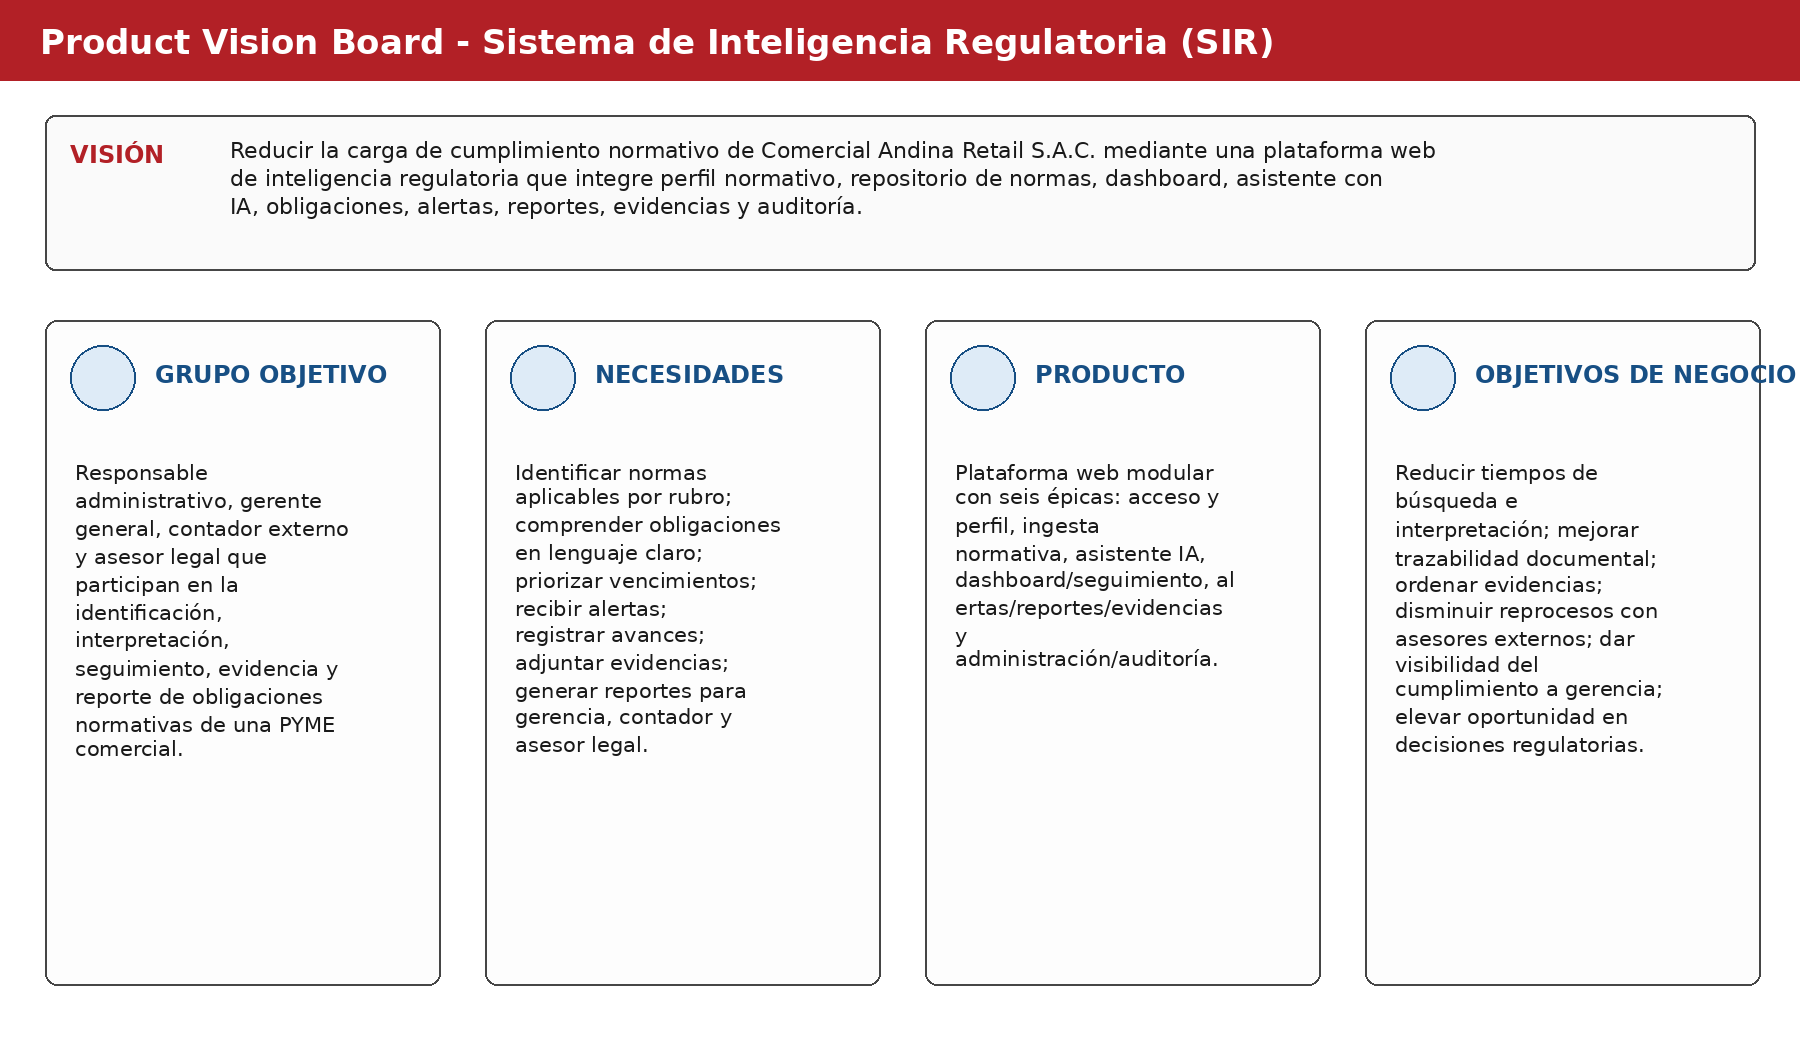
\includegraphics[width=0.95\textwidth,height=0.78\textheight,keepaspectratio]{figuras/cap3_product_vision_board.png}
\figurenote{Elaboración propia.}
\end{figure}

La visión del producto se resume en la siguiente declaración: implementar una plataforma de inteligencia regulatoria que permita a Comercial Andina Retail S.A.C. identificar obligaciones aplicables, interpretar cambios normativos en lenguaje claro, monitorear el estado de cumplimiento, recibir alertas oportunas y generar reportes con evidencia trazable de las fuentes oficiales consultadas. Esta visión responde a la necesidad de reducir tiempos de búsqueda, disminuir dependencia de interpretaciones no documentadas, ordenar el seguimiento de obligaciones y mejorar la oportunidad en la toma de decisiones de cumplimiento.

\subsection{Perfil del Usuario}\label{subsec:perfil-del-usuario}

El usuario principal del sistema es el responsable administrativo de la PYME, debido a que concentra la coordinación de declaraciones, licencias, comunicaciones con asesores externos y seguimiento de obligaciones ante entidades fiscalizadoras. La Figura~\ref{fig:cap3-perfil-usuario} presenta el perfil de usuario priorizado, considerando biografía, frase representativa, personalidad, preocupaciones, frustraciones y necesidades.

\begin{figure}[H]
\centering
\caption{Perfil del usuario principal del SIR}
\label{fig:cap3-perfil-usuario}
\vspace{0.35em}
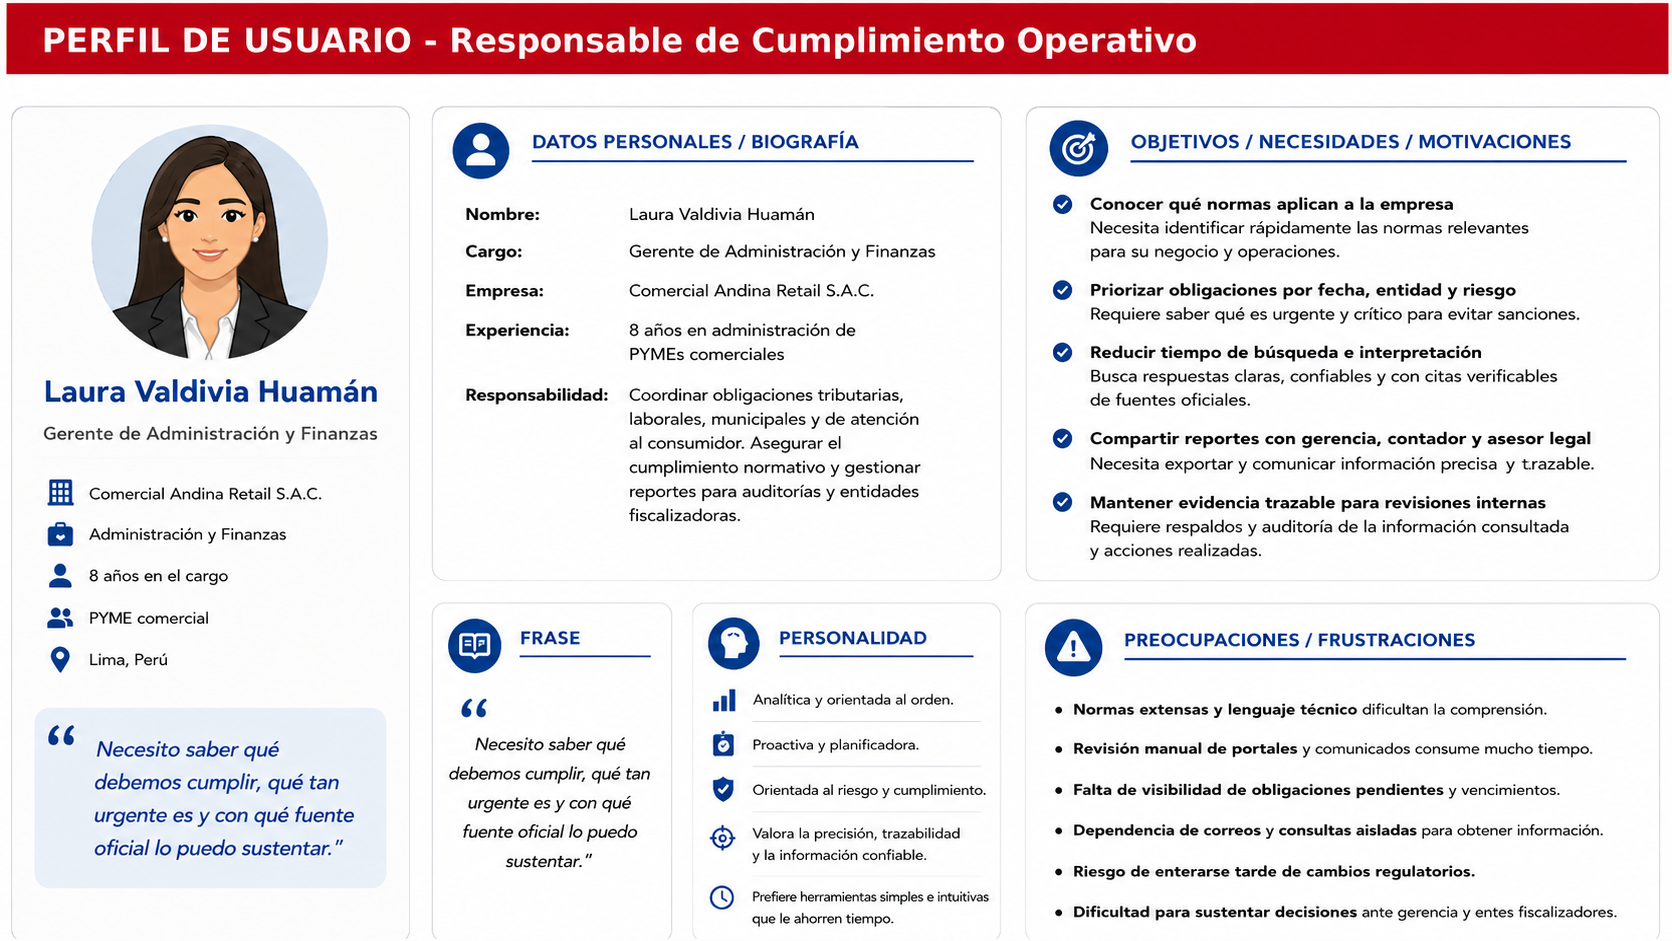
\includegraphics[width=0.95\textwidth,height=0.78\textheight,keepaspectratio]{figuras/cap3_perfil_usuario.png}
\figurenote{Elaboración propia.}
\end{figure}

Además del usuario principal, el producto considera usuarios secundarios que participan en el flujo de cumplimiento normativo. Estos usuarios no reemplazan el rol del responsable administrativo, pero intervienen en la revisión, validación o ejecución de acciones derivadas de las respuestas del SIR.

\begin{longtable}{p{0.24\textwidth}p{0.21\textwidth}p{0.28\textwidth}p{0.19\textwidth}}
\caption{Perfiles de usuario del SIR}\label{tab:cap3-perfiles-usuario}\\
\toprule
\textbf{Perfil} & \textbf{Rol en el proceso} & \textbf{Necesidad principal} & \textbf{Dolor actual} \\
\midrule
\endfirsthead
\toprule
\textbf{Perfil} & \textbf{Rol en el proceso} & \textbf{Necesidad principal} & \textbf{Dolor actual} \\
\midrule
\endhead
Responsable administrativo & Usuario líder y responsable operativo & Identificar obligaciones aplicables, fechas relevantes y acciones concretas de cumplimiento. & Búsqueda manual en múltiples fuentes y dificultad para interpretar lenguaje legal. \\
Contador externo & Validador tributario y asesor recurrente & Revisar respuestas, validar obligaciones tributarias y preparar declaraciones. & Recibe consultas repetitivas y con poca evidencia documental. \\
Gerente general & Decisor y responsable de priorización & Conocer riesgos de incumplimiento y estado general de obligaciones. & Falta de visibilidad ejecutiva sobre obligaciones pendientes. \\
Asesor legal externo & Especialista consultado en casos complejos & Revisar normas de mayor impacto o incertidumbre. & Debe reconstruir contexto y fuentes antes de emitir opinión. \\
\bottomrule
\end{longtable}

\subsection{Definición de Roles}\label{subsec:definicion-de-roles}

El proyecto se organiza bajo un esquema Scrum adaptado al tamaño del equipo de desarrollo y al alcance funcional de la solución. Los roles definidos aseguran la separación entre priorización funcional, coordinación del proceso ágil, desarrollo técnico, validación de calidad y retroalimentación del usuario líder.

\begin{longtable}{p{0.21\textwidth}p{0.22\textwidth}p{0.13\textwidth}p{0.36\textwidth}}
\caption{Definición de roles del proyecto}\label{tab:cap3-definicion-roles}\\
\toprule
\textbf{Rol} & \textbf{Responsable} & \textbf{Tiempo estimado} & \textbf{Responsabilidades} \\
\midrule
\endfirsthead
\toprule
\textbf{Rol} & \textbf{Responsable} & \textbf{Tiempo estimado} & \textbf{Responsabilidades} \\
\midrule
\endhead
Product Owner & Laura Valdivia Huamán & 180 horas & Priorizar el Product Backlog desde la perspectiva del negocio, validar el valor de cada incremento, aprobar criterios funcionales y mantener alineada la solución con las necesidades de cumplimiento de Comercial Andina Retail S.A.C. \\
Scrum Master & Jadir Hervias & 160 horas & Facilitar ceremonias Scrum, gestionar impedimentos, promover el cumplimiento del marco ágil y mantener la visibilidad del avance. \\
Líder técnico & Jadir Hervias & 220 horas & Definir lineamientos de arquitectura, seleccionar tecnologías, revisar integración entre frontend, backend, motor RAG y bases de datos. \\
Analista funcional & Khail Mogollón & 180 horas & Levantar requerimientos, modelar historias de usuario, criterios de aceptación, flujos funcionales y reglas de negocio. \\
Desarrollador backend/IA & Jadir Hervias & 300 horas & Implementar API, ingesta normativa, procesamiento de textos, embeddings, recuperación vectorial y generación de respuestas. \\
Desarrollador frontend & Khail Mogollón & 260 horas & Implementar interfaces de perfil empresarial, asistente regulatorio, dashboard, matriz de obligaciones, alertas, historial y reportes. \\
Analista QA & Equipo de desarrollo & 120 horas & Diseñar y ejecutar pruebas funcionales, pruebas de precisión, validación de citaciones, usabilidad y rendimiento. \\
Usuario líder & Responsable administrativo de Comercial Andina Retail S.A.C. & 60 horas & Validar prototipos, probar flujos del sistema, revisar dashboard, alertas, reportes, claridad de respuestas y aportar retroalimentación operativa. \\
Sponsor del proyecto & Gerencia general de Comercial Andina Retail S.A.C. & 40 horas & Aprobar alcance funcional, facilitar acceso a información operativa y validar la utilidad del sistema para el seguimiento del cumplimiento y la toma de decisiones. \\
\bottomrule
\end{longtable}

La designación del Product Owner recae en un representante funcional de la empresa y no en los integrantes del equipo de desarrollo. Esta separación permite que la priorización del producto responda a necesidades reales de negocio, mientras que Jadir Hervias y Khail Mogollón mantienen responsabilidades técnicas y funcionales de construcción, análisis y validación del sistema.

\subsection{Diseño Preliminar de la Solución}\label{subsec:diseno-preliminar-de-la-solucion}

El Product Canvas permite representar de manera integrada el objetivo del producto, las métricas de éxito, el grupo objetivo, el panorama general de la solución y los detalles funcionales de alto nivel. La Figura~\ref{fig:cap3-product-canvas} consolida el diseño preliminar del SIR y establece el puente entre las necesidades del usuario y las funcionalidades priorizadas en el Product Backlog.

\begin{figure}[H]
\centering
\caption{Product Canvas del SIR}
\label{fig:cap3-product-canvas}
\vspace{0.35em}
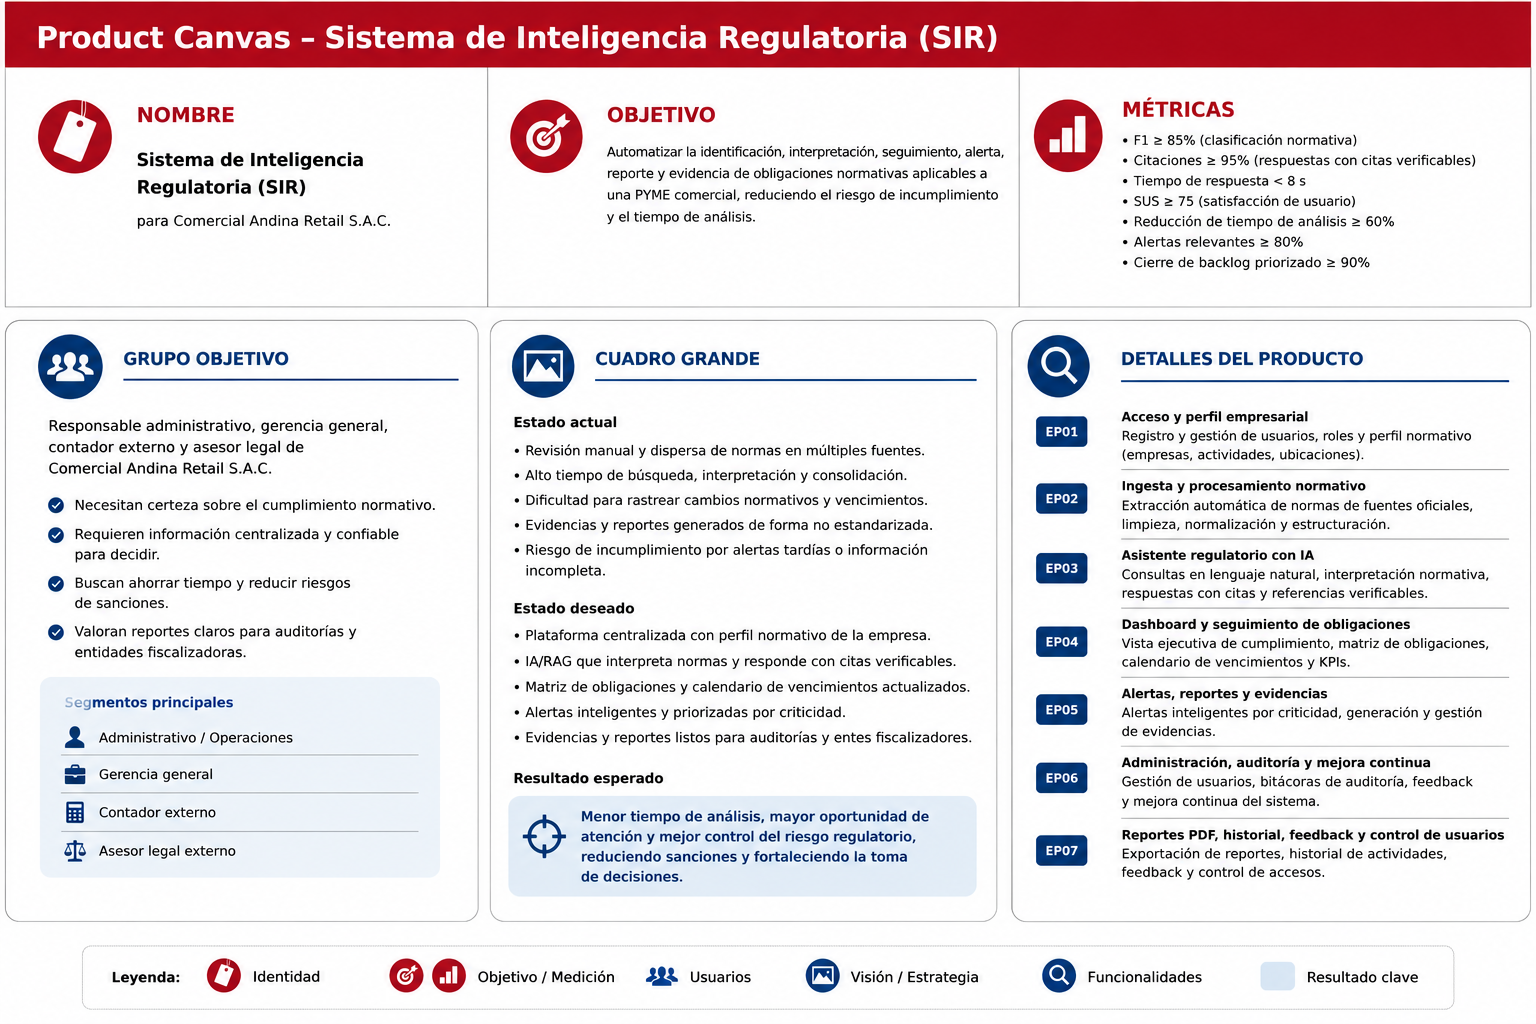
\includegraphics[width=0.95\textwidth,height=0.78\textheight,keepaspectratio]{figuras/cap3_product_canvas.png}
\figurenote{Elaboración propia.}
\end{figure}

A nivel conceptual, el SIR transforma el proceso de cumplimiento normativo de la PYME en siete capacidades principales. Primero, permite configurar un perfil empresarial con rubro, tamaño, ubicación y entidades reguladoras relevantes. Segundo, automatiza la ingesta y preparación del corpus normativo. Tercero, habilita consultas en lenguaje natural con respuestas trazables a fuentes oficiales. Cuarto, consolida obligaciones en una matriz de seguimiento con responsable, fecha, estado y evidencia. Quinto, presenta un dashboard ejecutivo con semáforos, indicadores y alertas por vencer. Sexto, genera reportes exportables para gerencia, contador externo o asesor legal. Séptimo, organiza evidencias, historial, auditoría y retroalimentación para sostener la mejora continua del proceso de cumplimiento.

\begin{longtable}{p{0.25\textwidth}p{0.33\textwidth}p{0.34\textwidth}}
\caption{Módulos funcionales de la solución SIR}\label{tab:cap3-modulos-sir}\\
\toprule
\textbf{Módulo} & \textbf{Propósito} & \textbf{Valor para la PYME} \\
\midrule
\endfirsthead
\toprule
\textbf{Módulo} & \textbf{Propósito} & \textbf{Valor para la PYME} \\
\midrule
\endhead
Perfil empresarial y normativo & Registrar rubro, tamaño, ubicación, entidades reguladoras y preferencias. & Permite contextualizar consultas, alertas y obligaciones según la realidad de la empresa. \\
Repositorio normativo & Ingerir, limpiar, clasificar y almacenar normas oficiales y fragmentos relevantes. & Reduce búsqueda manual y centraliza fuentes consultables. \\
Asistente regulatorio con IA & Responder consultas en lenguaje natural mediante RAG y citas verificables. & Facilita interpretación operativa sin perder trazabilidad de fuentes. \\
Dashboard de cumplimiento & Mostrar indicadores, obligaciones pendientes, alertas y semáforos por entidad. & Brinda visibilidad ejecutiva para priorizar acciones de cumplimiento. \\
Matriz de obligaciones & Registrar obligación, responsable, vencimiento, estado, evidencia y comentarios. & Convierte una respuesta normativa en una acción gestionable. \\
Sistema básico de alertas & Notificar cambios normativos, obligaciones por vencer y pendientes críticos. & Mejora oportunidad de respuesta ante riesgos de incumplimiento. \\
Reportes ejecutivos & Generar reportes PDF con consultas, respuestas, fuentes, estados y conclusiones operativas. & Facilita comunicación con gerencia, contador y asesor legal. \\
Repositorio de evidencias & Centralizar archivos, enlaces, constancias, capturas, respuestas y documentos asociados a cada obligación. & Permite sustentar acciones de cumplimiento y reducir pérdida de información. \\
Historial, auditoría y mejora continua & Registrar consultas, citaciones, reportes, calificaciones, cambios y acciones de usuarios. & Permite aprendizaje continuo, control interno y revisión posterior. \\
\bottomrule
\end{longtable}

\subsection{Prototipos Alto Nivel}\label{subsec:prototipos-alto-nivel}

Los prototipos de alto nivel representan las pantallas principales de la solución. No constituyen diseños finales de interfaz, sino artefactos funcionales que permiten validar navegación, estructura de información y acciones clave del usuario. La Figura~\ref{fig:cap3-prototipos} muestra los prototipos correspondientes al dashboard de cumplimiento, asistente regulatorio con IA, matriz de obligaciones, centro de alertas, reportes, repositorio de evidencias y perfil normativo de la empresa.

\begin{figure}[H]
\centering
\caption{Prototipos de alto nivel del SIR}
\label{fig:cap3-prototipos}
\vspace{0.35em}
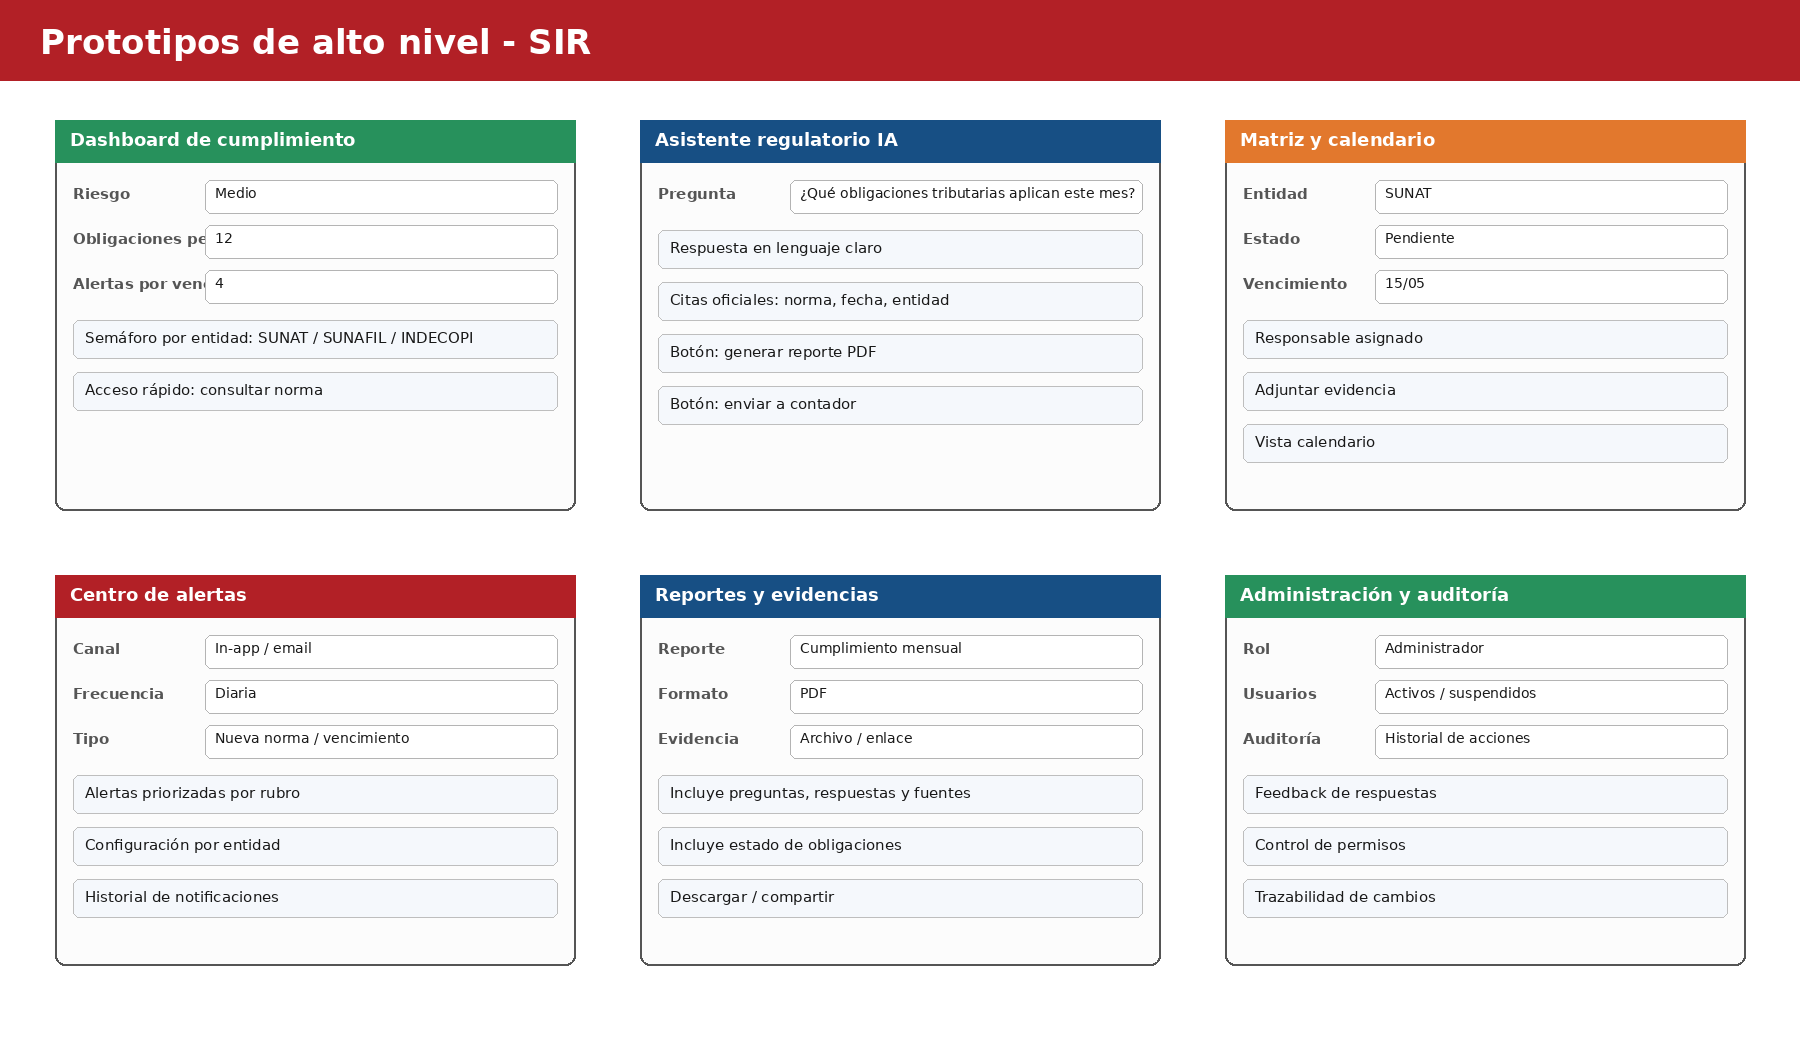
\includegraphics[width=0.95\textwidth,height=0.78\textheight,keepaspectratio]{figuras/cap3_prototipos.png}
\figurenote{Elaboración propia.}
\end{figure}

Las épicas funcionales asociadas a los prototipos son las siguientes:

\begin{itemize}
    \item \textbf{Épica 1: Gestión de acceso y perfil empresarial}. Permite registrar usuarios, autenticar accesos, administrar roles iniciales y configurar los datos base de la empresa.
    \item \textbf{Épica 2: Ingesta y procesamiento normativo}. Permite recolectar, limpiar, segmentar, clasificar y vectorizar normas oficiales para alimentar el repositorio normativo.
    \item \textbf{Épica 3: Asistente regulatorio con IA}. Permite realizar preguntas en lenguaje natural, recibir respuestas con citas verificables y contextualizar la interpretación según el perfil de la PYME.
    \item \textbf{Épica 4: Dashboard y seguimiento de obligaciones}. Permite visualizar indicadores de cumplimiento, semáforos por entidad, obligaciones pendientes y calendario de vencimientos.
    \item \textbf{Épica 5: Alertas, reportes y evidencias de cumplimiento}. Permite configurar alertas básicas, generar reportes PDF, adjuntar evidencias y organizar documentos de sustento por obligación.
    \item \textbf{Épica 6: Administración, auditoría y mejora continua}. Permite gestionar usuarios, permisos, historial de consultas, trazabilidad de acciones y retroalimentación para mejorar la calidad del sistema.
\end{itemize}

\subsection{Historias de Usuario}\label{subsec:historias-de-usuario}

Las historias de usuario se formulan con la estructura: \textit{Como} rol, \textit{necesito} funcionalidad, \textit{para} obtener valor de negocio. Esta estructura permite conectar las necesidades del usuario con entregables verificables y criterios de aceptación medibles.

\begin{longtable}{p{0.06\textwidth}p{0.18\textwidth}p{0.12\textwidth}p{0.22\textwidth}p{0.34\textwidth}}
\caption{Descripción de historias de usuario}\label{tab:cap3-historias-usuario}\\
\toprule
\textbf{N.\textsuperscript{o}} & \textbf{Épica} & \textbf{ID} & \textbf{Historia} & \textbf{Descripción de la historia de usuario} \\
\midrule
\endfirsthead
\toprule
\textbf{N.\textsuperscript{o}} & \textbf{Épica} & \textbf{ID} & \textbf{Historia} & \textbf{Descripción de la historia de usuario} \\
\midrule
\endhead
1 & EP01 & HU01 & Registro de usuario y empresa & Como responsable administrativo, necesito registrar mi usuario y los datos básicos de la empresa para acceder al SIR con información empresarial identificable. \\
2 & EP01 & HU02 & Autenticación y roles & Como usuario registrado, necesito iniciar sesión de forma segura para acceder solo a las funciones autorizadas. \\
3 & EP01 & HU03 & Configuración de perfil normativo & Como responsable administrativo, necesito configurar rubro, tamaño, ubicación y entidades relevantes para recibir información normativa aplicable. \\
4 & EP02 & HU04 & Ingesta automática de normas & Como sistema, necesito extraer normas oficiales de fuentes públicas para mantener actualizado el corpus normativo. \\
5 & EP02 & HU05 & Limpieza y normalización textual & Como sistema, necesito limpiar y normalizar textos legales para que puedan ser procesados por el motor de IA. \\
6 & EP02 & HU06 & Vectorización de documentos & Como sistema, necesito convertir fragmentos normativos en embeddings para habilitar búsqueda semántica. \\
7 & EP02 & HU07 & Clasificación normativa & Como sistema, necesito clasificar normas por entidad, rubro y tipo de obligación para mejorar la relevancia de recuperación. \\
8 & EP03 & HU08 & Consulta en lenguaje natural & Como responsable administrativo, necesito formular preguntas en lenguaje natural para entender obligaciones sin leer documentos extensos. \\
9 & EP03 & HU09 & Respuestas con citas verificables & Como usuario, necesito que cada respuesta incluya fuente oficial para validar la información utilizada. \\
10 & EP03 & HU10 & Consulta contextualizada & Como usuario PYME, necesito que las respuestas consideren el perfil de la empresa para saber si una norma aplica a mi caso. \\
11 & EP04 & HU11 & Dashboard de cumplimiento & Como gerente general, necesito visualizar indicadores, riesgos, alertas y obligaciones recientes para conocer el estado de cumplimiento. \\
12 & EP04 & HU14 & Seguimiento de obligaciones & Como responsable administrativo, necesito registrar estado, fecha, responsable y evidencia de atención de obligaciones para controlar el cumplimiento. \\
13 & EP04 & HU19 & Calendario de vencimientos & Como responsable administrativo, necesito visualizar obligaciones por fecha de vencimiento para priorizar acciones y evitar incumplimientos. \\
14 & EP05 & HU12 & Alertas regulatorias & Como responsable administrativo, necesito recibir alertas sobre cambios normativos y obligaciones por vencer para actuar oportunamente. \\
15 & EP05 & HU13 & Preferencias de notificación & Como usuario, necesito configurar frecuencia, entidades y medios de alerta para evitar saturación de información. \\
16 & EP05 & HU15 & Exportación de reportes & Como contador externo, necesito exportar respuestas, obligaciones y evidencias a PDF para sustentar revisiones y declaraciones. \\
17 & EP05 & HU20 & Repositorio de evidencias & Como responsable administrativo, necesito adjuntar y consultar documentos de sustento asociados a cada obligación para mantener evidencia ordenada. \\
18 & EP06 & HU16 & Historial y auditoría & Como usuario, necesito consultar el historial de preguntas, respuestas, fuentes y acciones para reutilizar evidencia y revisar decisiones. \\
19 & EP06 & HU17 & Feedback de respuestas & Como usuario líder, necesito calificar la utilidad de respuestas para mejorar el sistema y el dataset de validación. \\
20 & EP06 & HU18 & Administración de usuarios & Como administrador, necesito crear, editar o desactivar usuarios para mantener control de accesos. \\
\bottomrule
\end{longtable}

\subsubsection{Criterios de aceptación}\label{subsubsec:criterios-aceptacion}

Los criterios de aceptación establecen las condiciones mínimas que debe cumplir cada historia para ser considerada terminada. Se priorizan criterios verificables en pruebas funcionales, pruebas de integración, revisión de trazabilidad y validación con el usuario líder.

\begin{longtable}{p{0.13\textwidth}p{0.27\textwidth}p{0.52\textwidth}}
\caption{Criterios de aceptación principales}\label{tab:cap3-criterios-aceptacion}\\
\toprule
\textbf{ID} & \textbf{Historia} & \textbf{Criterios de aceptación} \\
\midrule
\endfirsthead
\toprule
\textbf{ID} & \textbf{Historia} & \textbf{Criterios de aceptación} \\
\midrule
\endhead
HU01 & Registro de usuario y empresa & Debe solicitar correo, contraseña, razón social y RUC; validar formato de correo y RUC de 11 dígitos; registrar fecha de alta; confirmar creación de cuenta. \\
HU02 & Autenticación y roles & Debe permitir login seguro, cierre de sesión, recuperación de contraseña y acceso diferenciado según rol. \\
HU03 & Configuración de perfil normativo & Debe registrar rubro CIIU, tamaño empresarial, ubicación y entidades de interés; debe permitir edición y guardar historial de cambios. \\
HU04 & Ingesta automática de normas & Debe ejecutar proceso programado, extraer PDF/HTML, almacenar metadatos y registrar errores de ingesta. \\
HU05 & Limpieza y normalización textual & Debe eliminar ruido, preservar estructura legal, normalizar caracteres y segmentar artículos o disposiciones. \\
HU06 & Vectorización de documentos & Debe generar embeddings, asociarlos al documento original y almacenarlos en la base vectorial con metadatos. \\
HU07 & Clasificación normativa & Debe asignar entidad, tipo de norma, rubro y tipo de obligación; debe permitir revisión manual de clasificaciones inciertas. \\
HU08 & Consulta en lenguaje natural & Debe aceptar preguntas en español, responder en menos de 8 segundos bajo carga normal e indicar cuando no exista información suficiente. \\
HU09 & Respuestas con citas verificables & Debe incluir número de norma, entidad emisora, fecha, fragmento consultado y enlace a la fuente oficial cuando esté disponible. \\
HU10 & Consulta contextualizada & Debe usar rubro, tamaño y ubicación de la empresa para indicar aplicabilidad, exclusiones o condiciones específicas. \\
HU11 & Dashboard de cumplimiento & Debe mostrar normas recientes, obligaciones pendientes, alertas por vencer, semáforos por entidad, accesos rápidos al asistente regulatorio y estado de cumplimiento. \\
HU14 & Seguimiento de obligaciones & Debe permitir registrar estado, responsable, fecha de atención, evidencia, comentarios y nivel de prioridad por obligación. \\
HU19 & Calendario de vencimientos & Debe mostrar obligaciones en vista mensual y semanal; debe resaltar vencimientos próximos y permitir filtrar por entidad, responsable y estado. \\
HU12 & Alertas regulatorias & Debe generar alertas ante nuevas normas, cambios relevantes u obligaciones próximas a vencer, y enviarlas por el medio configurado por el usuario. \\
HU13 & Preferencias de notificación & Debe permitir activar/desactivar alertas por entidad, frecuencia, tipo de norma, nivel de prioridad y canal de comunicación. \\
HU15 & Exportación de reportes & Debe generar PDF con pregunta, respuesta, fuentes, fecha de emisión, perfil usado, obligaciones relacionadas, evidencias asociadas y aviso de apoyo no vinculante. \\
HU20 & Repositorio de evidencias & Debe permitir adjuntar archivos o enlaces, asociarlos a una obligación, registrar fecha, usuario responsable y tipo de evidencia, y permitir descarga posterior. \\
HU16 & Historial y auditoría & Debe listar consultas con fecha, usuario, fuentes utilizadas, reportes generados y acciones realizadas; debe permitir búsqueda por palabra clave. \\
HU17 & Feedback de respuestas & Debe permitir calificación de utilidad, reporte de error y almacenamiento de feedback para análisis posterior. \\
HU18 & Administración de usuarios & Debe permitir crear, editar, suspender usuarios y asignar permisos sin exponer contraseñas. \\
\bottomrule
\end{longtable}

\subsection{Product Backlog Base}\label{subsec:product-backlog-base}

\subsubsection{Técnica de priorización}\label{subsubsec:tecnica-priorizacion}

Para ordenar el desarrollo de las historias de usuario se utiliza la técnica MoSCoW. Los requisitos \textit{Must Have} son indispensables para demostrar la solución mínima viable; los \textit{Should Have} aportan valor relevante pero pueden implementarse después del núcleo funcional; los \textit{Could Have} son mejoras deseables para ampliar experiencia de usuario, trazabilidad o administración.

\subsubsection{Técnica de estimación}\label{subsubsec:tecnica-estimacion}

La estimación del esfuerzo se realiza mediante Planning Poker, asignando puntos de historia según complejidad funcional, incertidumbre técnica, dependencias y riesgo de integración. La estimación se expresa en una escala relativa y permite planificar el alcance de los cuatro sprints del proyecto.

\begin{longtable}{p{0.07\textwidth}p{0.10\textwidth}p{0.28\textwidth}p{0.12\textwidth}p{0.12\textwidth}p{0.13\textwidth}p{0.10\textwidth}}
\caption{Product Backlog inicial}\label{tab:cap3-product-backlog}\\
\toprule
\textbf{N.\textsuperscript{o}} & \textbf{ID} & \textbf{Historia} & \textbf{Épica} & \textbf{Valor negocio} & \textbf{MoSCoW} & \textbf{Sprint} \\
\midrule
\endfirsthead
\toprule
\textbf{N.\textsuperscript{o}} & \textbf{ID} & \textbf{Historia} & \textbf{Épica} & \textbf{Valor negocio} & \textbf{MoSCoW} & \textbf{Sprint} \\
\midrule
\endhead
1 & HU04 & Ingesta automática de normas & EP02 & 100 & Must & 1 \\
2 & HU05 & Limpieza y normalización textual & EP02 & 100 & Must & 1 \\
3 & HU06 & Vectorización de documentos & EP02 & 100 & Must & 1 \\
4 & HU01 & Registro de usuario y empresa & EP01 & 95 & Must & 1 \\
5 & HU02 & Autenticación y roles & EP01 & 95 & Must & 1 \\
6 & HU03 & Configuración de perfil normativo & EP01 & 95 & Must & 2 \\
7 & HU08 & Consulta en lenguaje natural & EP03 & 100 & Must & 2 \\
8 & HU09 & Respuestas con citas verificables & EP03 & 100 & Must & 2 \\
9 & HU10 & Consulta contextualizada & EP03 & 95 & Must & 2 \\
10 & HU07 & Clasificación normativa & EP02 & 90 & Should & 3 \\
11 & HU11 & Dashboard de cumplimiento & EP04 & 90 & Should & 3 \\
12 & HU14 & Seguimiento de obligaciones & EP04 & 85 & Should & 3 \\
13 & HU19 & Calendario de vencimientos & EP04 & 80 & Should & 3 \\
14 & HU12 & Alertas regulatorias & EP05 & 90 & Should & 3 \\
15 & HU13 & Preferencias de notificación & EP05 & 75 & Could & 4 \\
16 & HU15 & Exportación de reportes & EP05 & 80 & Could & 4 \\
17 & HU20 & Repositorio de evidencias & EP05 & 80 & Should & 4 \\
18 & HU16 & Historial y auditoría & EP06 & 80 & Should & 4 \\
19 & HU17 & Feedback de respuestas & EP06 & 70 & Could & 4 \\
20 & HU18 & Administración de usuarios & EP06 & 70 & Could & 4 \\
\bottomrule
\end{longtable}

\subsection{Tablero Scrum Base y Roadmap del Producto}\label{subsec:tablero-scrum-roadmap}

El tablero Scrum base organiza el flujo de trabajo en cinco estados: Product Backlog, Pendiente, En proceso, En pruebas y Terminado. Esta estructura facilita la visibilidad del avance, la identificación de bloqueos y el control de calidad por historia de usuario. La Figura~\ref{fig:cap3-scrum-board} presenta el tablero base propuesto.

\begin{figure}[H]
\centering
\caption{Tablero Scrum base del SIR}
\label{fig:cap3-scrum-board}
\vspace{0.35em}
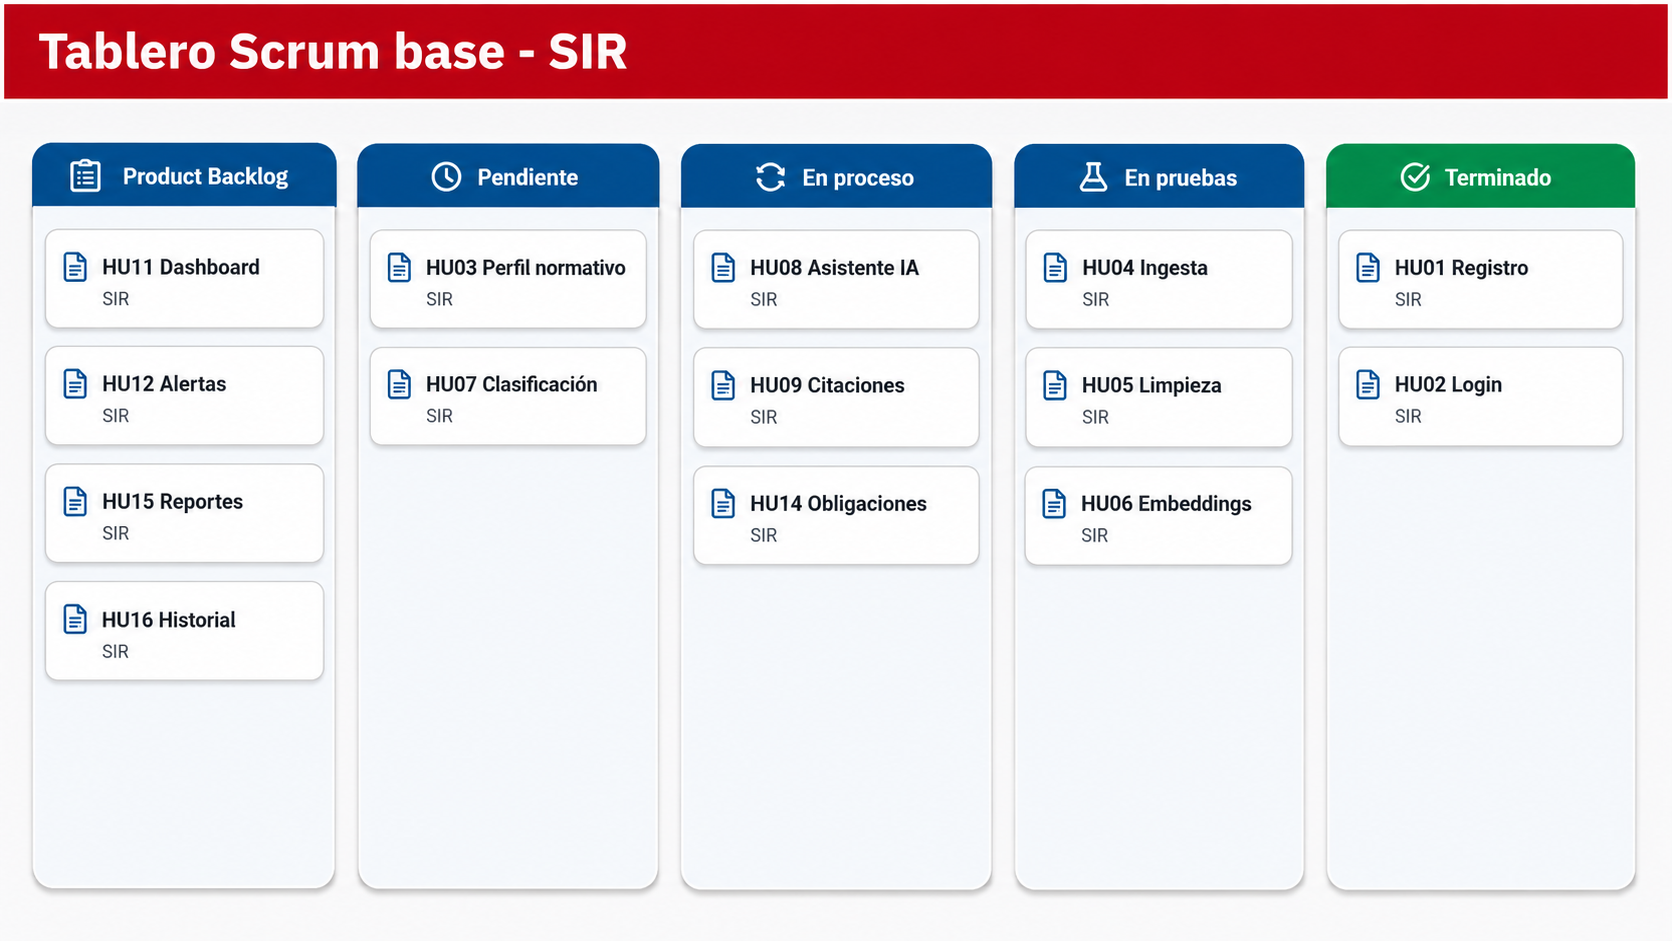
\includegraphics[width=0.95\textwidth,height=0.78\textheight,keepaspectratio]{figuras/cap3_scrum_board.png}
\figurenote{Elaboración propia.}
\end{figure}

El Product Roadmap distribuye los incrementos funcionales en cuatro sprints. Cada sprint entrega un objetivo verificable, un conjunto de características y métricas de aceptación. La Figura~\ref{fig:cap3-product-roadmap} presenta el roadmap del producto.

\begin{figure}[H]
\centering
\caption{Product Roadmap del SIR}
\label{fig:cap3-product-roadmap}
\vspace{0.35em}
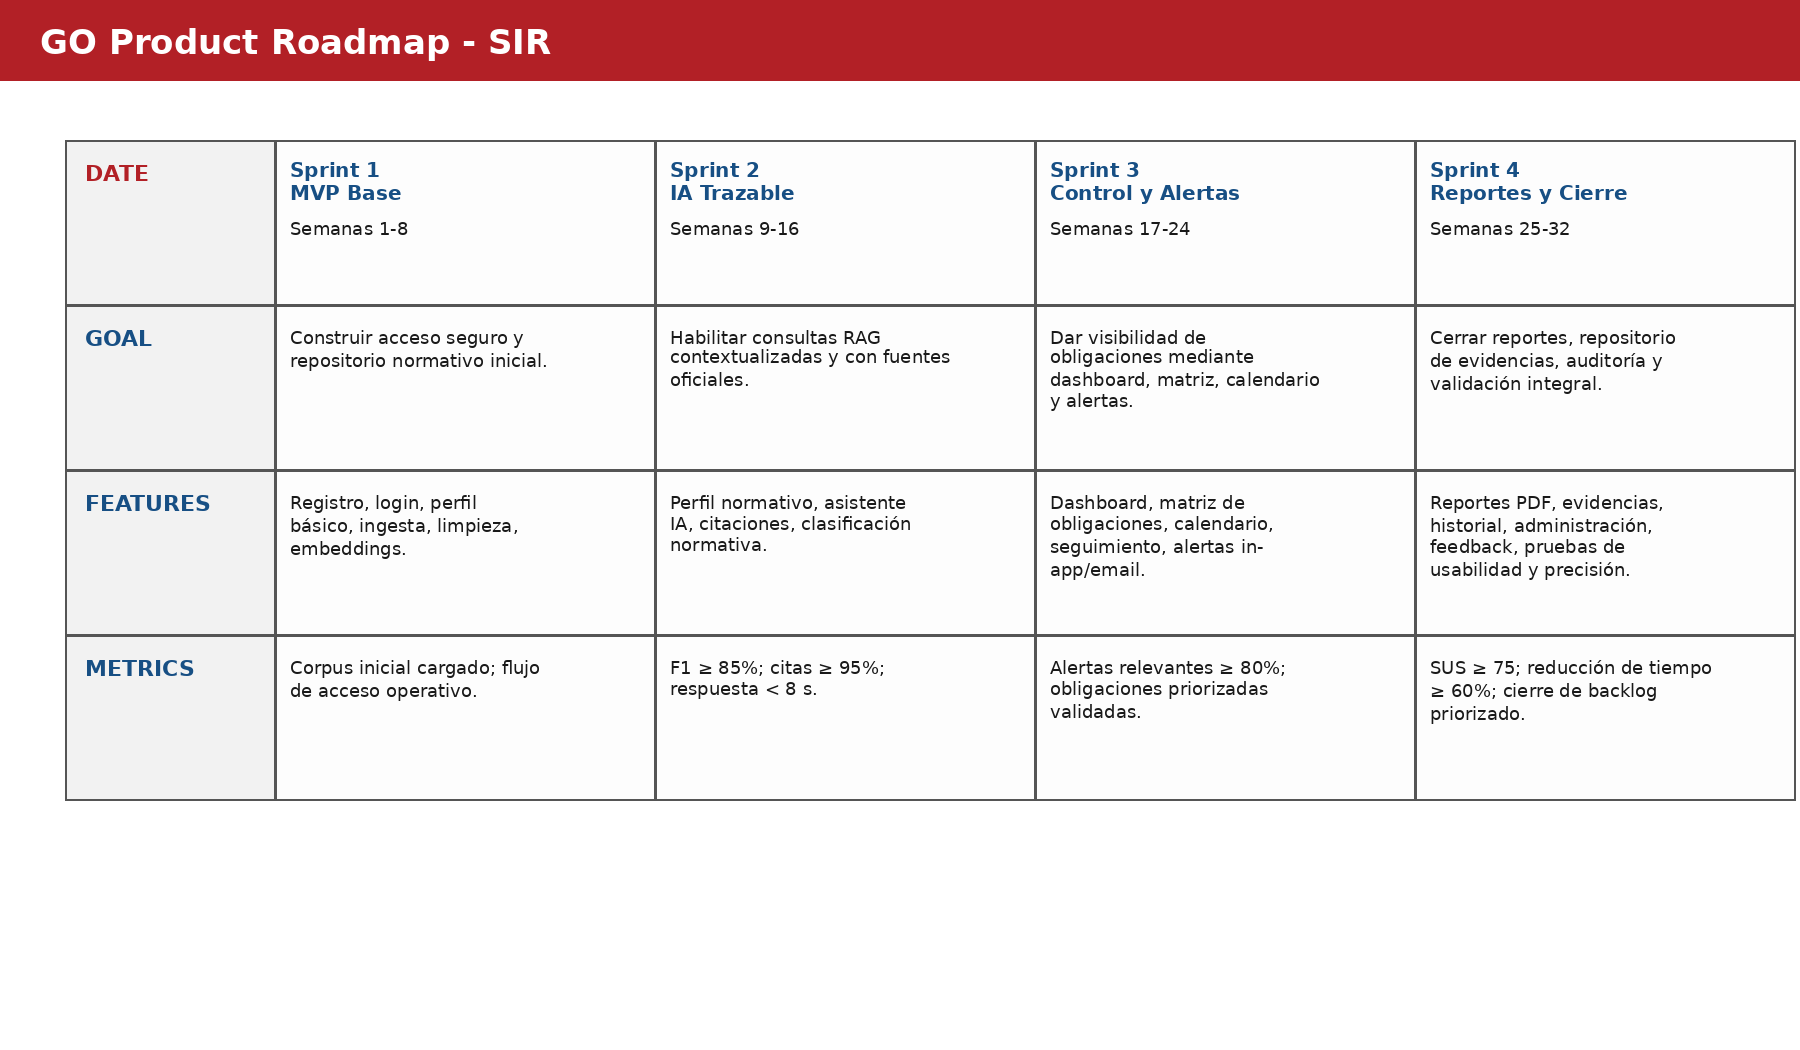
\includegraphics[width=0.95\textwidth,height=0.78\textheight,keepaspectratio]{figuras/cap3_product_roadmap.png}
\figurenote{Elaboración propia.}
\end{figure}

\begin{longtable}{p{0.14\textwidth}p{0.28\textwidth}p{0.30\textwidth}p{0.20\textwidth}}
\caption{Roadmap resumido por sprint}\label{tab:cap3-roadmap-sprint}\\
\toprule
\textbf{Sprint} & \textbf{Meta} & \textbf{Características principales} & \textbf{Métrica de control} \\
\midrule
\endfirsthead
\toprule
\textbf{Sprint} & \textbf{Meta} & \textbf{Características principales} & \textbf{Métrica de control} \\
\midrule
\endhead
Sprint 1 & Construir el núcleo de ingesta normativa y acceso seguro. & Registro, login, scraper inicial, limpieza textual, embeddings y almacenamiento. & Corpus cargado y flujo de acceso operativo. \\
Sprint 2 & Habilitar consultas RAG con respuestas trazables. & Perfil empresarial, asistente regulatorio, recuperación semántica, citaciones y contexto del perfil. & F1 ≥ 85\%, citas ≥ 95\%, respuesta < 8 s. \\
Sprint 3 & Incorporar personalización, dashboard, seguimiento y alertas. & Clasificación normativa, panel de obligaciones, calendario de vencimientos, alertas y seguimiento. & Alertas relevantes ≥ 80\% y dashboard validado por usuario líder. \\
Sprint 4 & Cerrar funcionalidades complementarias y validación. & Reportes PDF, repositorio de evidencias, historial, feedback, administración y pruebas finales. & SUS ≥ 75 y reducción de tiempo ≥ 60\%. \\
\bottomrule
\end{longtable}

\subsection{Otras consideraciones}\label{subsec:otras-consideraciones}

El alcance funcional del proyecto se limita a apoyar la interpretación operativa de normas y el seguimiento de obligaciones de cumplimiento. El SIR no emite opinión legal vinculante, no sustituye el criterio profesional de un abogado o contador, y no ejecuta declaraciones tributarias ni trámites ante entidades públicas.

\begin{longtable}{p{0.30\textwidth}p{0.62\textwidth}}
\caption{Restricciones del proyecto}\label{tab:cap3-restricciones}\\
\toprule
\textbf{Restricción} & \textbf{Descripción} \\
\midrule
\endfirsthead
\toprule
\textbf{Restricción} & \textbf{Descripción} \\
\midrule
\endhead
Restricción funcional & El sistema brinda asistencia interpretativa y trazabilidad documental, pero no reemplaza asesoría legal, contable o tributaria vinculante. \\
Restricción de fuentes & La calidad del resultado depende de la disponibilidad, estructura y acceso a fuentes oficiales, comunicados y normas públicas. \\
Restricción técnica & La precisión del motor RAG depende de la calidad de extracción, segmentación, embeddings y prompts de generación. \\
Restricción económica & Se priorizan servicios cloud y herramientas de bajo costo para mantener viabilidad económica en una PYME. \\
Restricción de tiempo & El desarrollo se organiza en cuatro sprints, por lo que las funcionalidades complementarias se priorizan según valor de negocio. \\
Restricción de seguridad & El sistema debe proteger datos de usuarios, RUC, historial de consultas y documentos internos bajo principios de minimización y control de acceso. \\
\bottomrule
\end{longtable}

\section{Arquitectura de software}\label{sec:arquitectura-de-software}

La arquitectura del SIR se diseña para integrar una aplicación web, una API de negocio, un motor de recuperación aumentada por generación, una base de datos transaccional, una base vectorial y un proceso de ingesta normativa. La arquitectura prioriza trazabilidad, mantenibilidad, seguridad, escalabilidad y bajo costo operativo.

\subsection{Arquitectura Técnica Base}\label{subsec:arquitectura-tecnica-base}

\subsubsection{Diagrama conceptual}\label{subsubsec:diagrama-conceptual}

El diagrama conceptual muestra la relación entre los usuarios, la aplicación web, la API del SIR, el orquestador RAG, los servicios de IA y las fuentes normativas. Como se observa en la Figura~\ref{fig:cap3-diagrama-conceptual}, el usuario interactúa con el sistema mediante consultas o alertas, mientras que el backend coordina recuperación de información, generación de respuestas y almacenamiento de evidencia.

\begin{figure}[H]
\centering
\caption{Diagrama conceptual TO-BE del SIR}
\label{fig:cap3-diagrama-conceptual}
\vspace{0.35em}
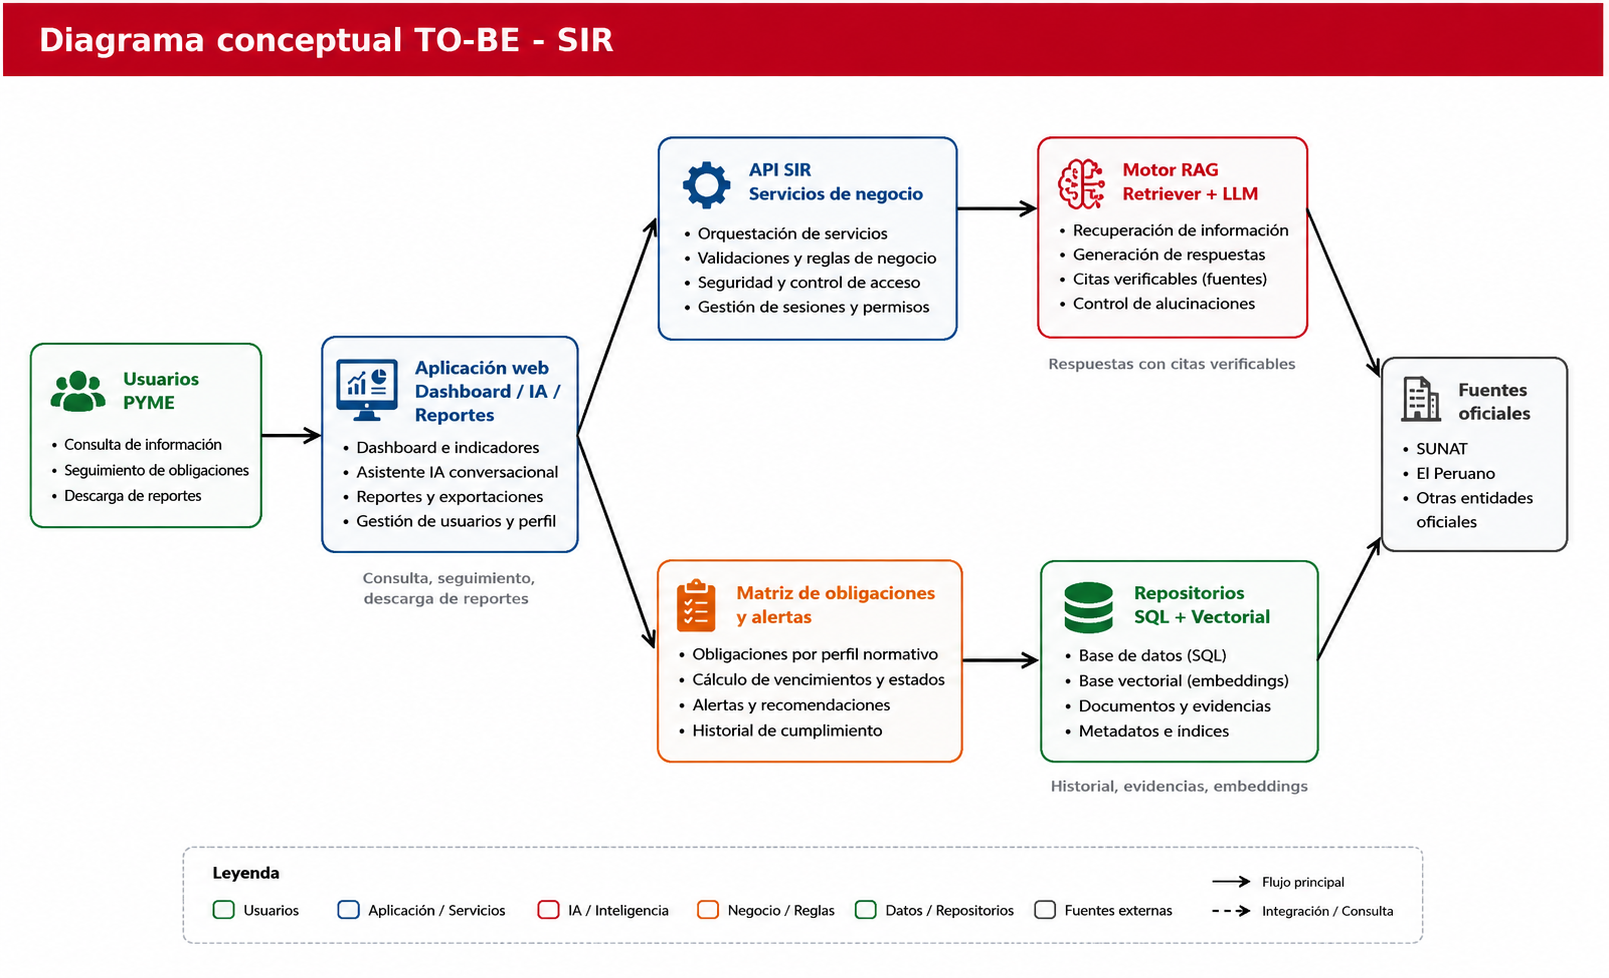
\includegraphics[width=0.95\textwidth,height=0.78\textheight,keepaspectratio]{figuras/cap3_diagrama_conceptual.png}
\figurenote{Elaboración propia.}
\end{figure}

\subsubsection{Diagrama físico}\label{subsubsec:diagrama-fisico}

La arquitectura física se plantea sobre servicios cloud de bajo costo y componentes administrados, a fin de reducir la carga operativa de infraestructura. La Figura~\ref{fig:cap3-db-fisica} muestra una propuesta de despliegue con frontend en CDN, API backend, worker de ingesta, base transaccional, base vectorial y servicios externos de IA.

\begin{figure}[H]
\centering
\caption{Arquitectura física de despliegue del SIR}
\label{fig:cap3-db-fisica}
\vspace{0.35em}
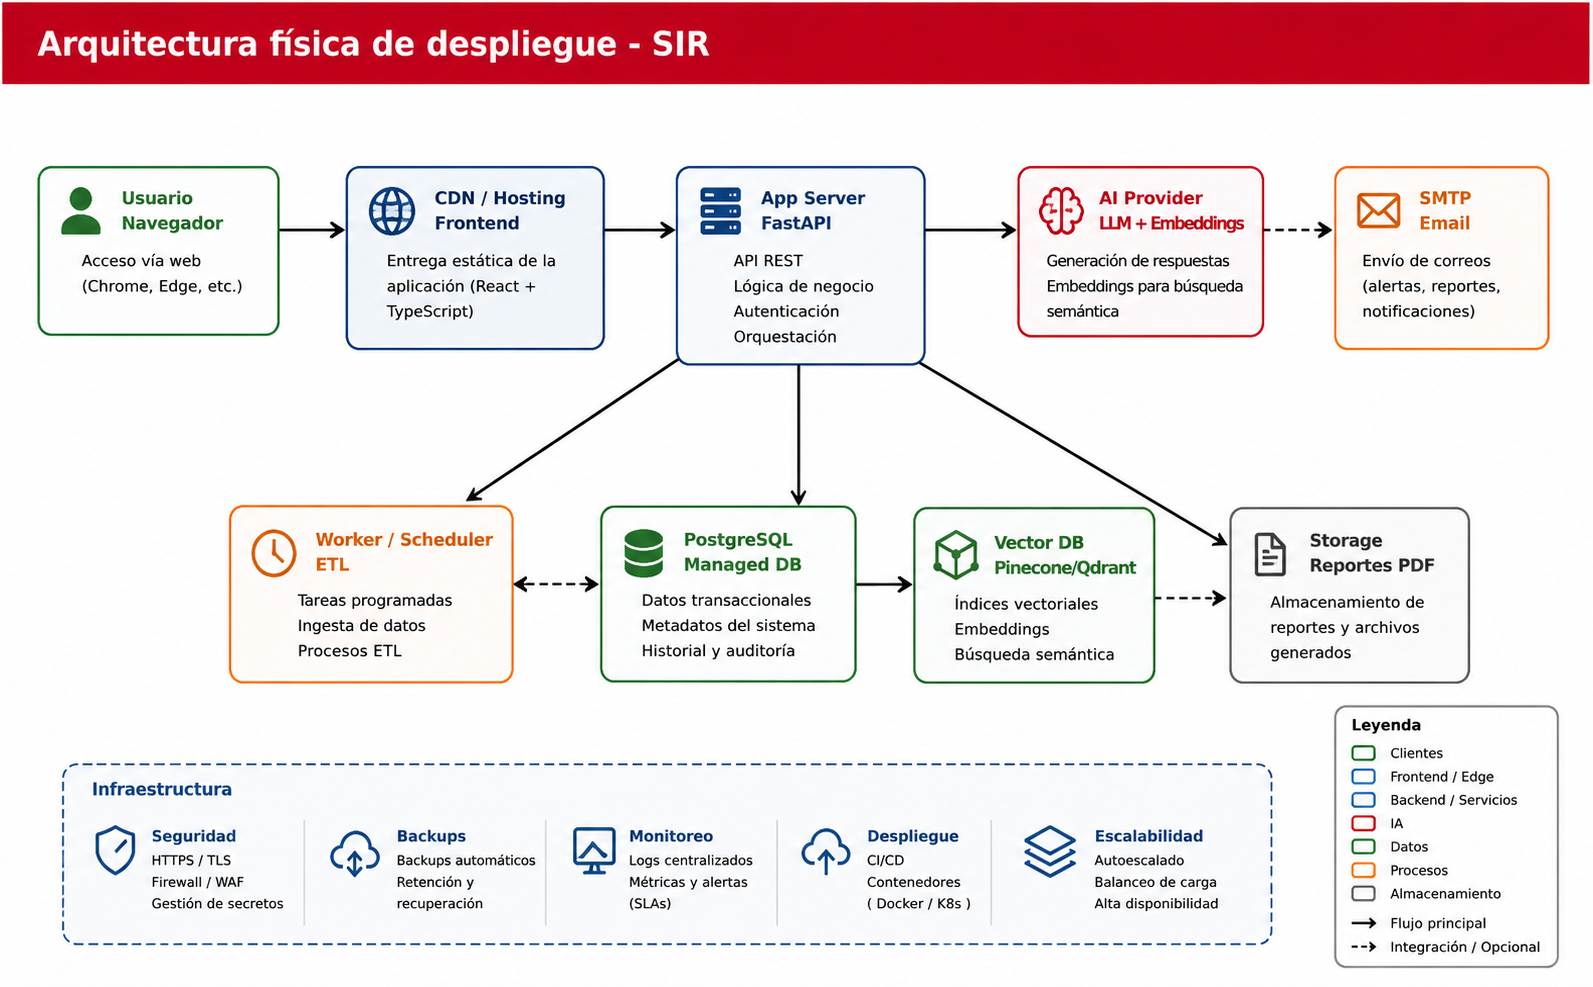
\includegraphics[width=0.95\textwidth,height=0.78\textheight,keepaspectratio]{figuras/cap3_db_fisica.png}
\figurenote{Elaboración propia.}
\end{figure}

\subsubsection{Diagrama lógico}\label{subsubsec:diagrama-logico}

El diagrama lógico organiza el sistema en capas de presentación, aplicación, motor de IA, datos transaccionales, datos vectoriales e ingesta normativa. Esta separación facilita la mantenibilidad, permite escalar componentes de manera independiente y reduce el acoplamiento entre la interfaz de usuario y los servicios de inteligencia artificial.

\begin{figure}[H]
\centering
\caption{Diagrama lógico de la solución SIR}
\label{fig:cap3-diagrama-logico}
\vspace{0.35em}
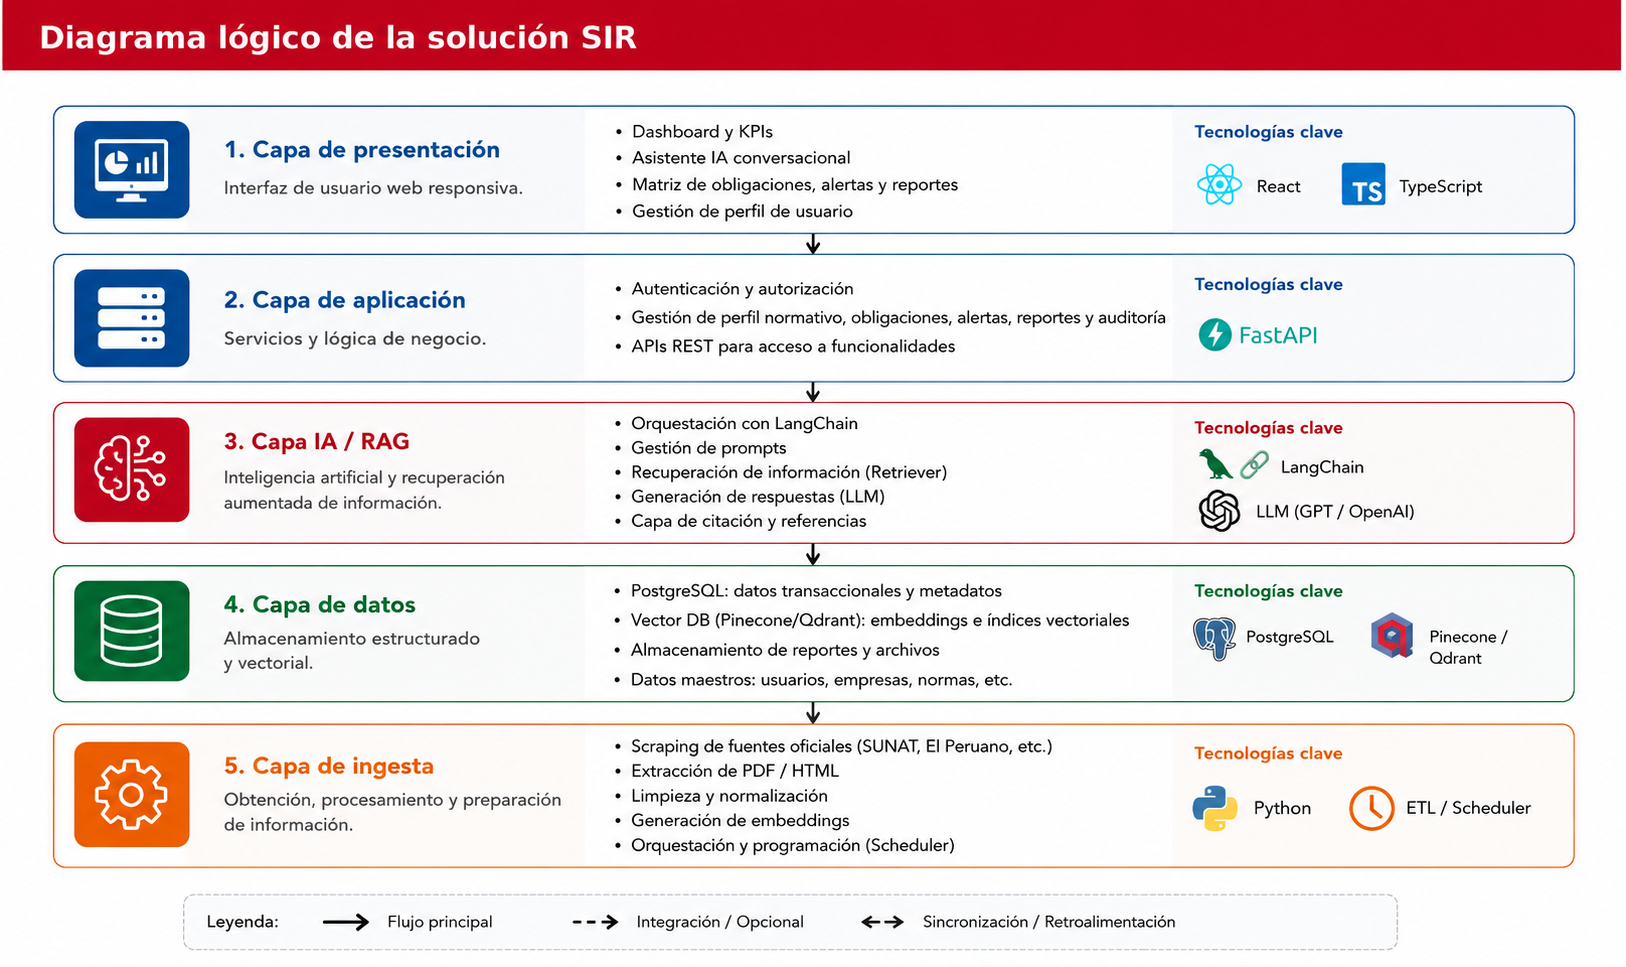
\includegraphics[width=0.95\textwidth,height=0.78\textheight,keepaspectratio]{figuras/cap3_diagrama_logico.png}
\figurenote{Elaboración propia.}
\end{figure}

\begin{longtable}{p{0.26\textwidth}p{0.26\textwidth}p{0.40\textwidth}}
\caption{Tecnologías consideradas en la arquitectura base}\label{tab:cap3-tecnologias}\\
\toprule
\textbf{Componente} & \textbf{Tecnología} & \textbf{Justificación} \\
\midrule
\endfirsthead
\toprule
\textbf{Componente} & \textbf{Tecnología} & \textbf{Justificación} \\
\midrule
\endhead
Frontend & React, TypeScript, TailwindCSS & Permite construir interfaces web modulares, mantenibles y responsivas. \\
Backend/API & Python, FastAPI & Facilita servicios REST, validación de datos, documentación automática e integración con librerías de IA. \\
Orquestación RAG & LangChain & Provee componentes para loaders, splitters, retrievers, prompts y cadenas de generación. \\
Modelo generativo & GPT-4 o modelo LLM equivalente & Permite generación de respuestas en lenguaje natural con control mediante contexto recuperado. \\
Embeddings & Modelo de embeddings compatible con el proveedor IA & Permite representar fragmentos normativos en vectores semánticos para búsqueda por similitud. \\
Base transaccional & PostgreSQL & Almacena usuarios, empresas, perfiles, historial, obligaciones, alertas y evidencias. \\
Base vectorial & Pinecone o Qdrant & Permite búsqueda semántica de fragmentos normativos y recuperación Top-K. \\
Ingesta normativa & Python, PyMuPDF, BeautifulSoup, scheduler & Automatiza extracción, limpieza y actualización del corpus normativo. \\
Despliegue & Vercel/Render/Supabase o servicios cloud equivalentes & Reduce costo operativo y facilita despliegue incremental de la solución. \\
\bottomrule
\end{longtable}

\subsection{Arquitectura Técnica Específica}\label{subsec:arquitectura-tecnica-especifica}

Para documentar la arquitectura técnica específica se utiliza el modelo C4, porque permite representar el sistema en niveles progresivos: contexto, contenedores y componentes. Estas vistas se complementan con la arquitectura lógica de datos y la arquitectura física de despliegue.

\subsubsection{Diagrama de contexto}\label{subsubsec:diagrama-contexto}

El diagrama de contexto identifica al SIR como sistema central y muestra su interacción con usuarios internos y externos, así como con fuentes regulatorias. La Figura~\ref{fig:cap3-c4-contexto} evidencia que el sistema no opera de manera aislada, sino que se articula con entidades públicas, fuentes oficiales y usuarios responsables de la ejecución de acciones de cumplimiento.

\begin{figure}[H]
\centering
\caption{Diagrama de contexto del SIR}
\label{fig:cap3-c4-contexto}
\vspace{0.35em}
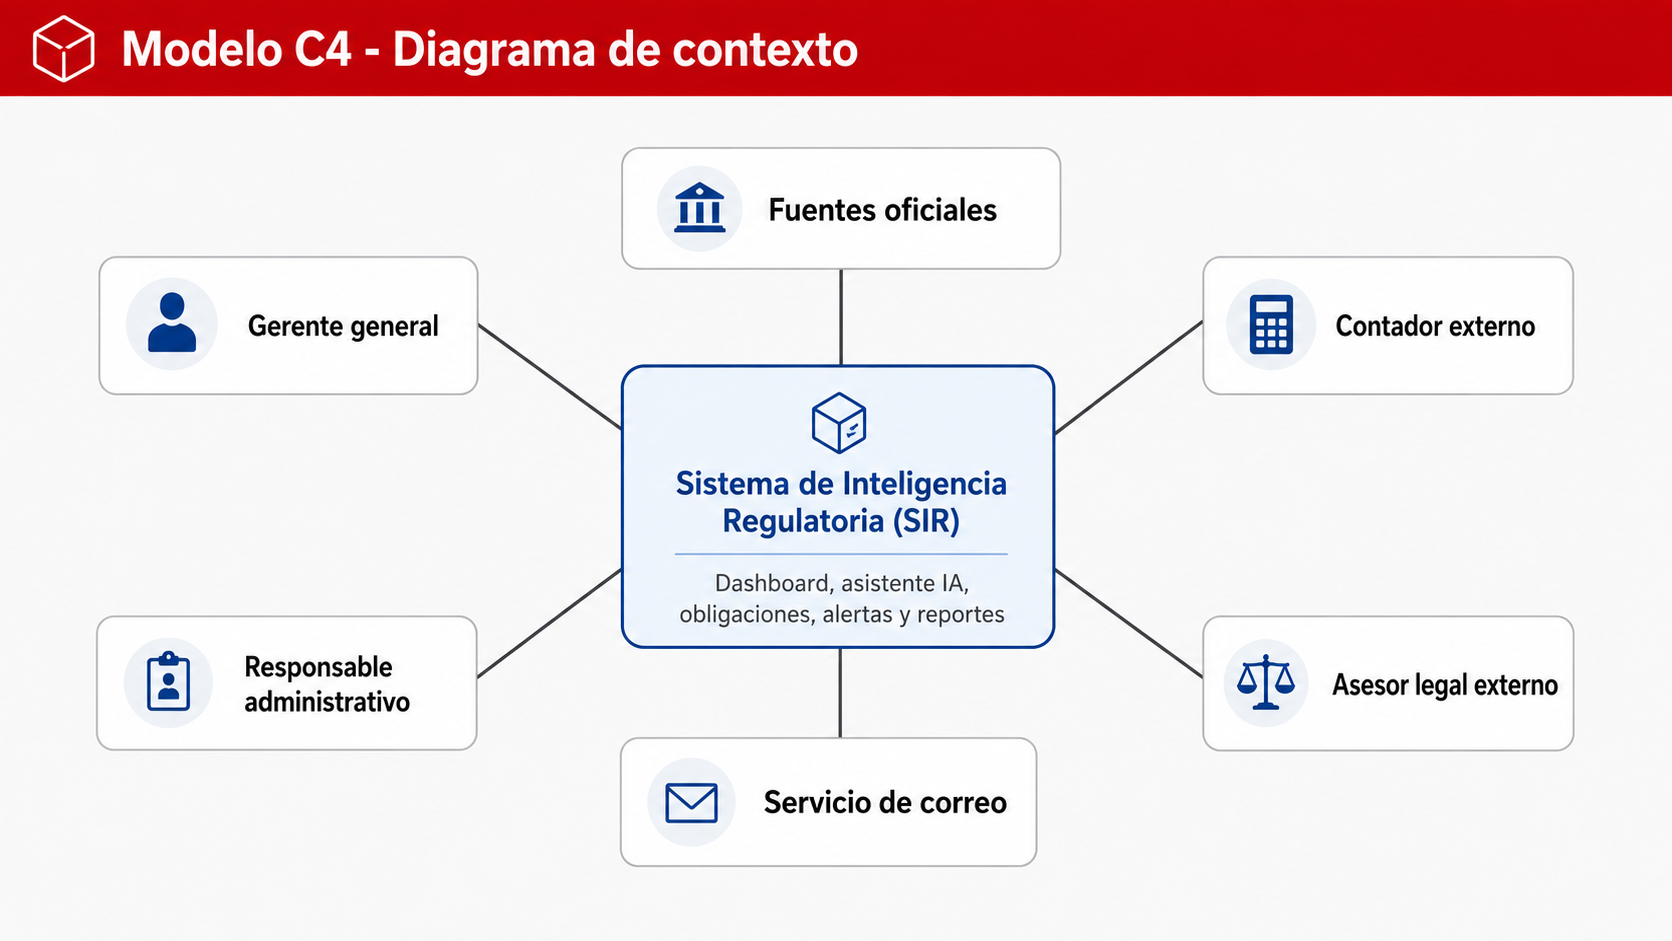
\includegraphics[width=0.95\textwidth,height=0.78\textheight,keepaspectratio]{figuras/cap3_c4_contexto.png}
\figurenote{Elaboración propia, bajo el enfoque del modelo C4.}
\end{figure}

\subsubsection{Diagrama de contenedores}\label{subsubsec:diagrama-contenedores}

La vista de contenedores descompone el sistema en aplicaciones y servicios desplegables. Como se presenta en la Figura~\ref{fig:cap3-c4-contenedores}, la aplicación web se comunica con la API REST, la cual coordina el motor RAG, el servicio de ingesta, la base transaccional, la base vectorial y el servicio de notificaciones.

\begin{figure}[H]
\centering
\caption{Diagrama de contenedores del SIR}
\label{fig:cap3-c4-contenedores}
\vspace{0.35em}
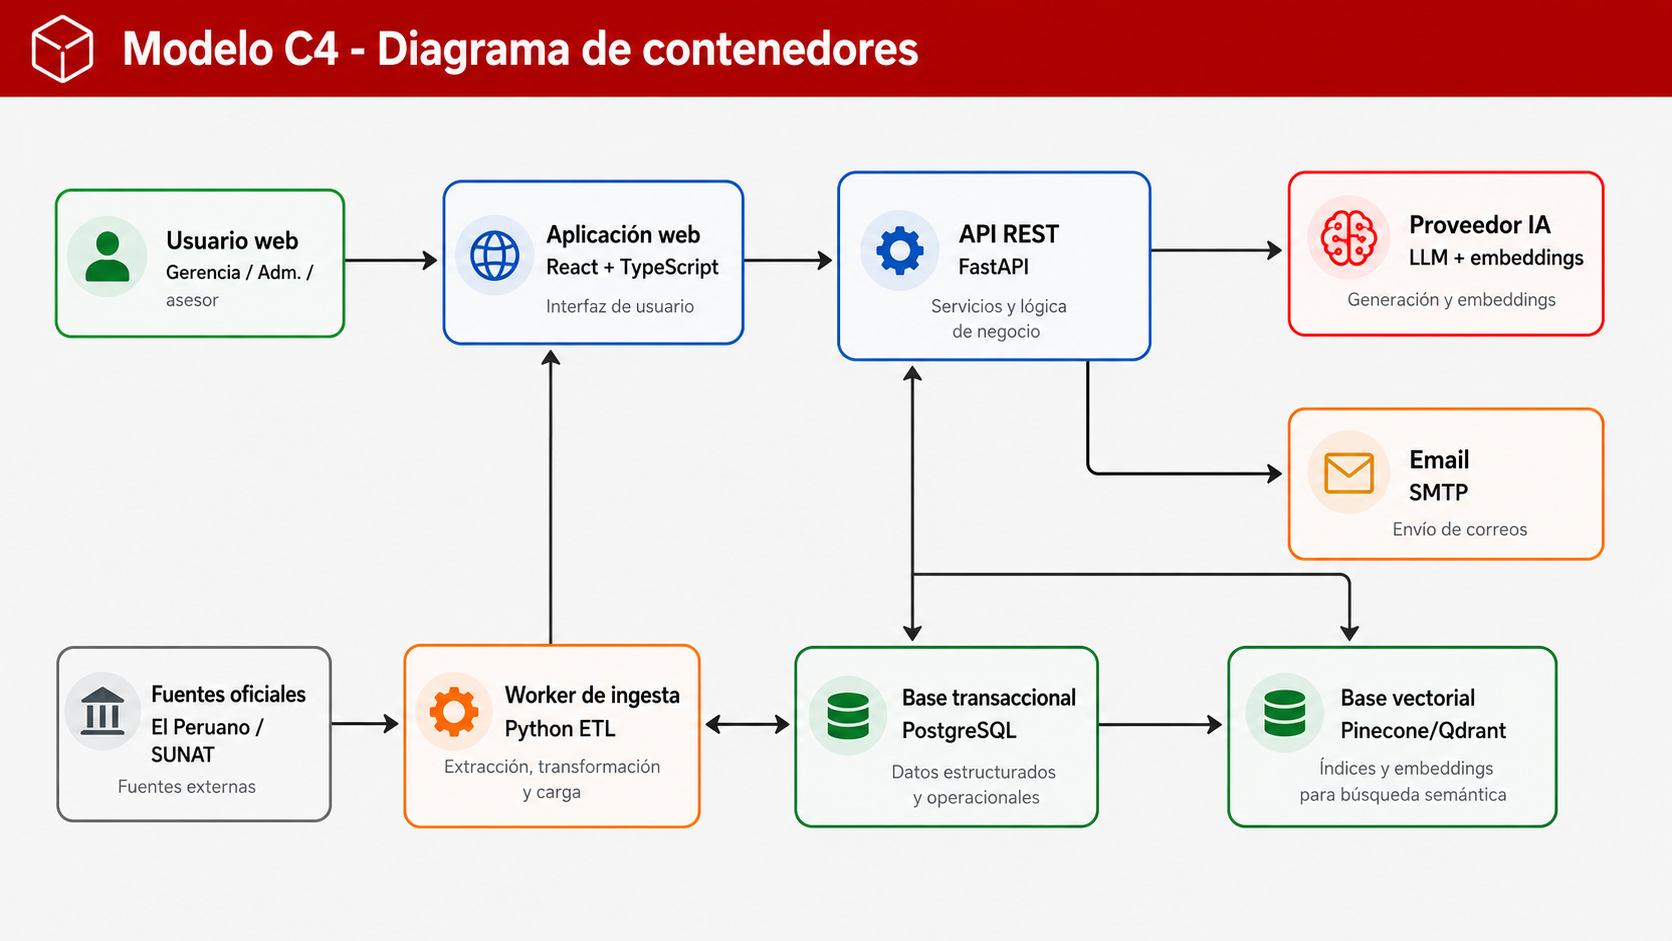
\includegraphics[width=0.95\textwidth,height=0.78\textheight,keepaspectratio]{figuras/cap3_c4_contenedores.png}
\figurenote{Elaboración propia, bajo el enfoque del modelo C4.}
\end{figure}

\subsubsection{Diagrama de componentes}\label{subsubsec:diagrama-componentes}

La vista de componentes detalla los módulos internos de la API y del motor de IA. La Figura~\ref{fig:cap3-c4-componentes} muestra servicios de autenticación, perfil, chat, alertas, reportes, orquestación RAG, recuperación semántica, capa de citación, procesamiento ETL, clasificación normativa y planificación de tareas.

\begin{figure}[H]
\centering
\caption{Diagrama de componentes del SIR}
\label{fig:cap3-c4-componentes}
\vspace{0.35em}
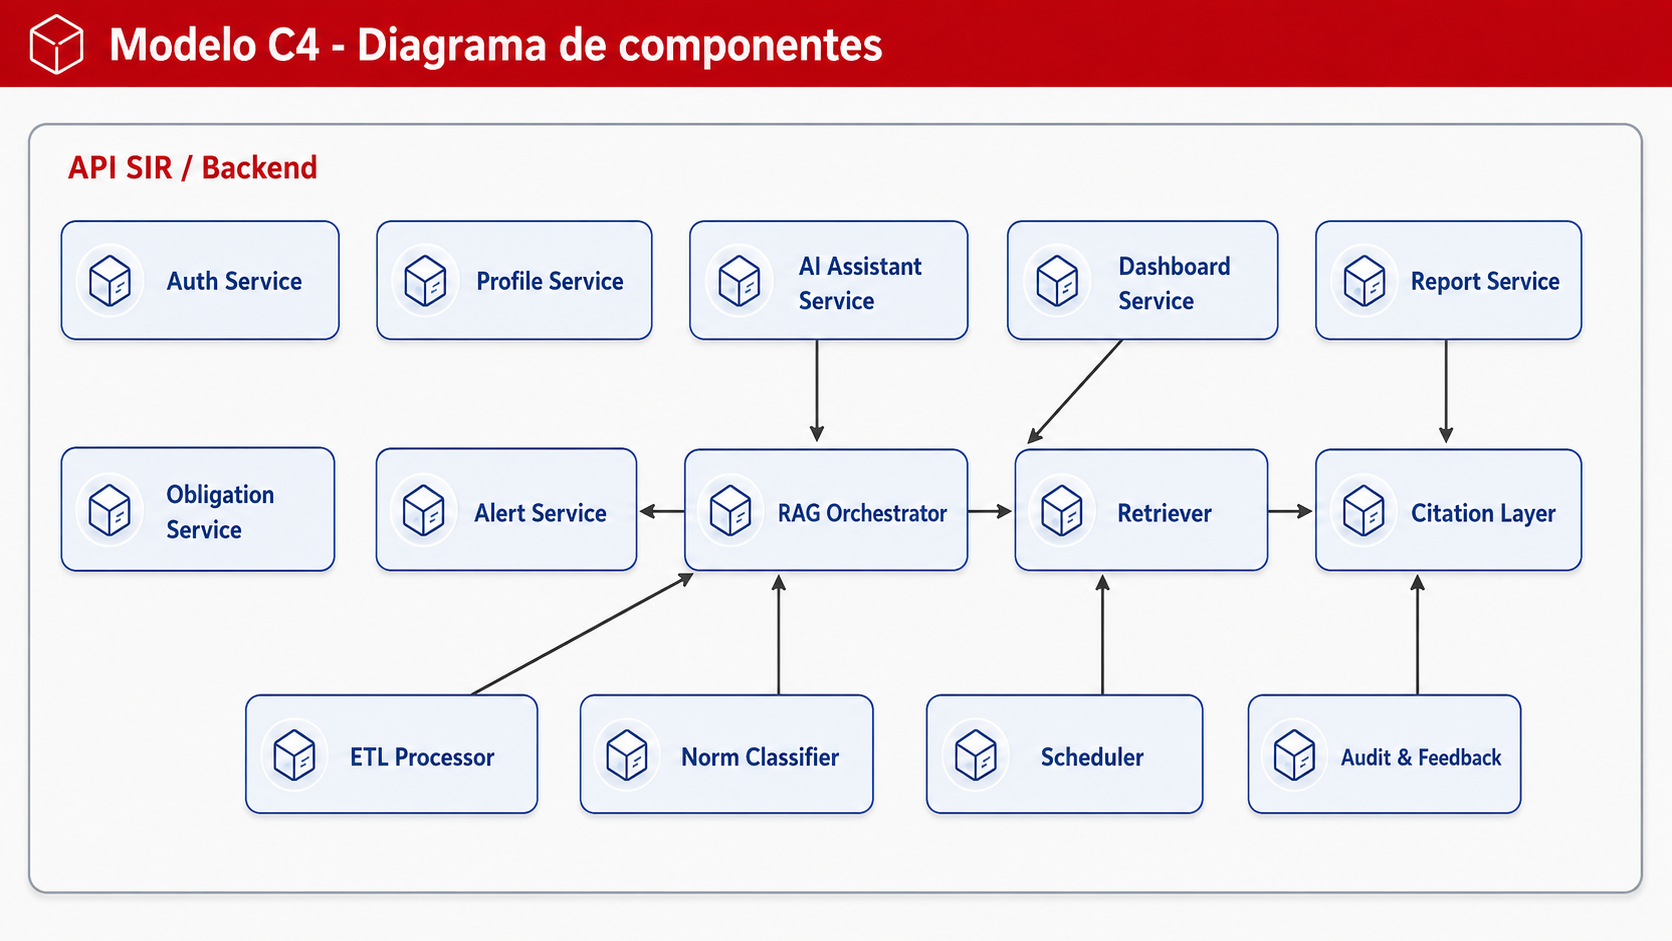
\includegraphics[width=0.95\textwidth,height=0.78\textheight,keepaspectratio]{figuras/cap3_c4_componentes.png}
\figurenote{Elaboración propia, bajo el enfoque del modelo C4.}
\end{figure}

\subsubsection{Arquitectura lógica de datos}\label{subsubsec:arquitectura-logica-datos}

La arquitectura lógica de datos define las entidades principales necesarias para soportar las funcionalidades del SIR. La Figura~\ref{fig:cap3-db-logica} presenta entidades relacionadas con usuarios, empresas, perfil normativo, normas, fragmentos normativos, consultas, citaciones y alertas. Esta estructura permite mantener trazabilidad entre una respuesta generada y los fragmentos normativos utilizados.

\begin{figure}[H]
\centering
\caption{Arquitectura lógica de datos del SIR}
\label{fig:cap3-db-logica}
\vspace{0.35em}
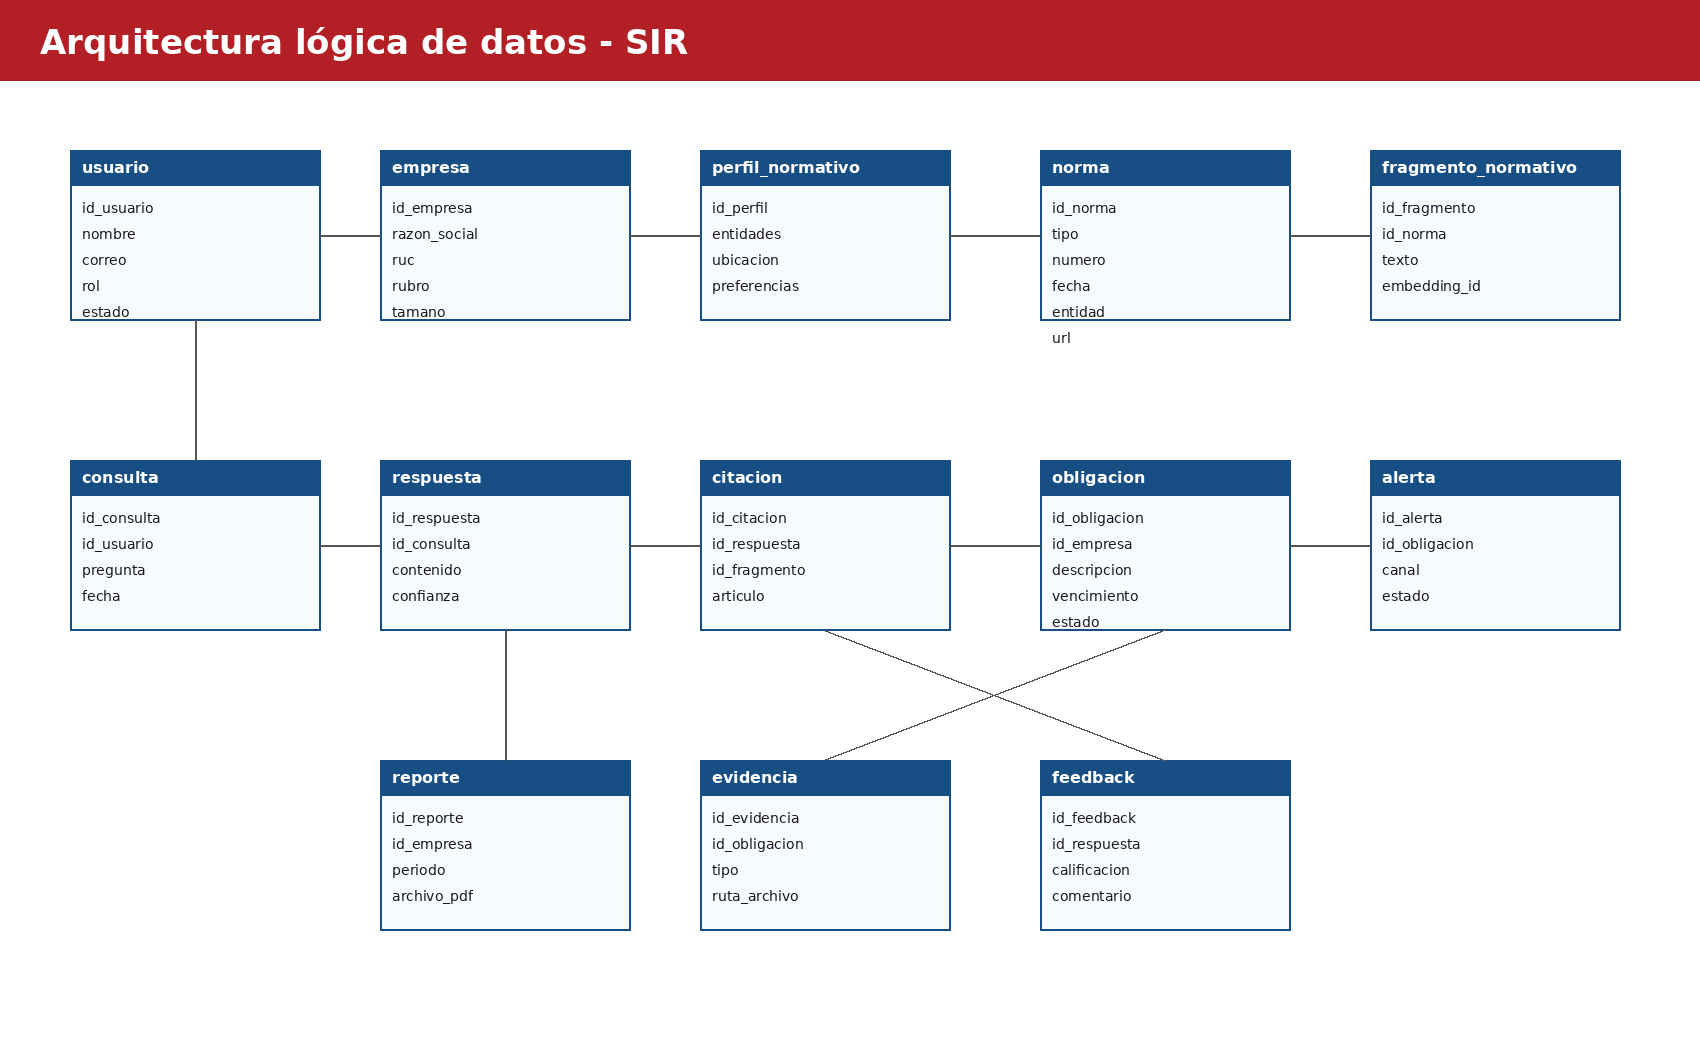
\includegraphics[width=0.95\textwidth,height=0.78\textheight,keepaspectratio]{figuras/cap3_db_logica.png}
\figurenote{Elaboración propia.}
\end{figure}

\subsubsection{Atributos de calidad de software}\label{subsubsec:atributos-calidad-software}

Los atributos de calidad permiten validar que la arquitectura no solo cubra funcionalidades, sino también condiciones operativas relevantes para una solución RegTech. La Tabla~\ref{tab:cap3-atributos-calidad} define escenarios y metas medibles para desempeño, disponibilidad, seguridad, mantenibilidad, escalabilidad, trazabilidad y usabilidad.

\begin{longtable}{p{0.20\textwidth}p{0.42\textwidth}p{0.30\textwidth}}
\caption{Atributos de calidad de software}\label{tab:cap3-atributos-calidad}\\
\toprule
\textbf{Atributo} & \textbf{Escenario} & \textbf{Meta} \\
\midrule
\endfirsthead
\toprule
\textbf{Atributo} & \textbf{Escenario} & \textbf{Meta} \\
\midrule
\endhead
Desempeño & El usuario realiza una consulta normativa con contexto empresarial. & Respuesta menor a 8 segundos bajo carga normal. \\
Disponibilidad & El usuario requiere consultar obligaciones durante horario operativo. & Disponibilidad mensual igual o superior a 99\%. \\
Seguridad & El sistema almacena datos de usuario, RUC, historial de consultas y evidencias. & Autenticación, control de roles, cifrado en tránsito y hashing de contraseñas. \\
Trazabilidad & Una respuesta generada por IA debe ser verificable. & Al menos 95\% de respuestas con fuente oficial, fecha, entidad y fragmento citado. \\
Mantenibilidad & El equipo debe incorporar cambios normativos o mejoras del prompt sin afectar todo el sistema. & Componentes desacoplados, versionamiento y despliegue controlado. \\
Escalabilidad & Aumenta el volumen de normas y consultas. & Separación entre API, base vectorial y worker de ingesta para escalar por componente. \\
Usabilidad & El usuario líder valida la facilidad de uso de la solución. & SUS igual o superior a 75 puntos. \\
\bottomrule
\end{longtable}

\subsubsection{Vistas de arquitectura}\label{subsubsec:vistas-arquitectura}

La documentación arquitectónica del SIR se organiza en las siguientes vistas:

\begin{itemize}
    \item \textbf{Vista de contexto}: delimita el sistema, los usuarios y las fuentes externas.
    \item \textbf{Vista de contenedores}: identifica aplicaciones, servicios y repositorios desplegables.
    \item \textbf{Vista de componentes}: describe módulos internos de backend, RAG, ingesta y alertas.
    \item \textbf{Vista de datos}: modela entidades transaccionales, fragmentos normativos, embeddings, consultas y citaciones.
    \item \textbf{Vista de despliegue}: representa infraestructura física o cloud requerida para operar la solución.
\end{itemize}

\subsubsection{Modelo de documentación}\label{subsubsec:modelo-documentacion}

El modelo de documentación combina C4 para comunicar la arquitectura desde distintos niveles de abstracción y el enfoque de atributos de calidad para justificar decisiones técnicas. Esta combinación permite que el diseño sea comprensible para usuarios de negocio y, al mismo tiempo, verificable por el equipo técnico encargado de la implementación.


\chapter{Gestión del Proyecto}\label{cap:7-gestion-del-proyecto}

El presente capítulo describe la gestión del proyecto siguiendo el marco PMBOK®, integrado con la operación ágil descrita en el Capítulo 3. Se documentan los planes de gestión por área de conocimiento (alcance, cronograma, costos, calidad, riesgos), la ejecución y el monitoreo a lo largo de PI-1 y PI-2.

\section{Planificación del Proyecto}\label{sec:planificacion-del-proyecto}

\textit{[PENDIENTE] Desarrollar el contenido de esta sección.}

\subsection{Plan de Gestión del Alcance (EDT)}\label{subsec:plan-de-gestion-del-alcance-edt}

\textbf{Definición del proyecto}

\begin{longtable}[]{@{}
  >{\raggedright\arraybackslash}p{(\columnwidth - 2\tabcolsep) * \real{0.5000}}
  >{\raggedright\arraybackslash}p{(\columnwidth - 2\tabcolsep) * \real{0.5000}}@{}}
\caption{Definición del proyecto}\\
\toprule\noalign{}
\begin{minipage}[b]{\linewidth}\raggedright
Atributo
\end{minipage} & \begin{minipage}[b]{\linewidth}\raggedright
Detalle
\end{minipage} \\
\midrule\noalign{}
\endhead
\bottomrule\noalign{}
\endlastfoot
Nombre & Sistema de Inteligencia Regulatoria (SIR) \\
Cliente / PO & Khail Mogollón -- PYMEs peruanas \\
Stakeholder principal & Editora Perú -- Daniel Espejo \\
Duración & 32 semanas (8 meses, 2 ciclos académicos) \\
Equipo & 2 personas (Hervias, Mogollón) \\
Objetivo & Plataforma RAG para interpretar normas legales y reducir carga de cumplimiento en PYMEs. \\
\end{longtable}

\textbf{Entregables principales}

\begin{itemize}
\item
  Memoria de investigación (PI-1 y PI-2).
\item
  Plataforma SIR con chatbot RAG, perfil, alertas e ingesta automatizada.
\item
  Documentación de arquitectura (modelo C4 y vistas 4+1).
\item
  Plan de pruebas y reportes de validación.
\item
  Material de presentación final por ciclo.
\end{itemize}

\textbf{Criterios de Aceptación del Producto}

\begin{longtable}[]{@{}
  >{\raggedright\arraybackslash}p{(\columnwidth - 4\tabcolsep) * \real{0.3335}}
  >{\raggedright\arraybackslash}p{(\columnwidth - 4\tabcolsep) * \real{0.3333}}
  >{\raggedright\arraybackslash}p{(\columnwidth - 4\tabcolsep) * \real{0.3332}}@{}}
\caption{Criterios de aceptación del producto}\\
\toprule\noalign{}
\begin{minipage}[b]{\linewidth}\raggedright
Criterio
\end{minipage} & \begin{minipage}[b]{\linewidth}\raggedright
Métrica
\end{minipage} & \begin{minipage}[b]{\linewidth}\raggedright
Meta
\end{minipage} \\
\midrule\noalign{}
\endhead
\bottomrule\noalign{}
\endlastfoot
Precisión del chatbot & F1-Score & ≥ 0.85 \\
Cobertura de citaciones & \% respuestas con fuente & ≥ 95\% \\
Tiempo de respuesta & Latencia p95 & \textless{} 8 seg \\
Usabilidad & SUS & ≥ 75 puntos \\
Disponibilidad & Uptime & ≥ 99\% \\
\end{longtable}

\textbf{Restricciones, supuestos y exclusiones}

\begin{itemize}
\item
  Restricción: presupuesto limitado y dedicación parcial del equipo.
\item
  Restricción: dependencia de la disponibilidad pública de El Peruano.
\item
  Supuesto: acceso continuo a APIs de OpenAI con créditos académicos.
\item
  Exclusión: emisión de opinión legal vinculante.
\item
  Exclusión: integración con ERPs internos de PYMEs (fuera de alcance).
\end{itemize}

\subsection{Plan de Gestión del Cronograma}\label{subsec:plan-de-gestion-del-cronograma}

\begin{longtable}[]{@{}
  >{\raggedright\arraybackslash}p{(\columnwidth - 6\tabcolsep) * \real{0.2501}}
  >{\raggedright\arraybackslash}p{(\columnwidth - 6\tabcolsep) * \real{0.2499}}
  >{\raggedright\arraybackslash}p{(\columnwidth - 6\tabcolsep) * \real{0.2498}}
  >{\raggedright\arraybackslash}p{(\columnwidth - 6\tabcolsep) * \real{0.2502}}@{}}
\caption{Hitos del proyecto}\\
\toprule\noalign{}
\begin{minipage}[b]{\linewidth}\raggedright
Hito
\end{minipage} & \begin{minipage}[b]{\linewidth}\raggedright
Semana
\end{minipage} & \begin{minipage}[b]{\linewidth}\raggedright
Ciclo
\end{minipage} & \begin{minipage}[b]{\linewidth}\raggedright
Descripción
\end{minipage} \\
\midrule\noalign{}
\endhead
\bottomrule\noalign{}
\endlastfoot
Aprobación de alcance y diseño preliminar & Sem 1 & PI-1 & Validación con asesor y stakeholder \\
Cierre Sprint 1 & Sem 8 & PI-1 & Pipeline + autenticación \\
Cierre Sprint 2 / Sustentación PI-1 & Sem 16 & PI-1 & Chatbot + perfil; demo PI-1 \\
Cierre Sprint 3 & Sem 24 & PI-2 & Personalización + alertas básicas \\
Cierre Sprint 4 / Sustentación PI-2 & Sem 32 & PI-2 & Funcionalidades de valor agregado y memoria final \\
\end{longtable}

\pendiente{Adjuntar diagrama de Gantt detallado por sprint y semana.}

\subsection{Plan de Gestión de Costos}\label{subsec:plan-de-gestion-de-costos}

El detalle del presupuesto, flujos por sprint y distribución por ciclo académico se encuentra en el Capítulo 6. Las consideraciones de control son:

\begin{itemize}
\item
  Monitoreo semanal del consumo de APIs (dashboard OpenAI/AWS).
\item
  Reporte mensual de ejecución vs. presupuesto.
\item
  Activación de plan de contingencia si el gasto supera el 80\% antes del día 20 del mes.
\item
  Re-priorización del backlog ante desviaciones significativas.
\end{itemize}

\subsection{Plan de Gestión de Calidad}\label{subsec:plan-de-gestion-de-calidad}

\textbf{Política de Calidad}

El proyecto adopta el estándar ISO/IEC 25010 para calidad de producto de software, complementado con prácticas de QA propias del marco ágil y los lineamientos del PMBOK®. Las características priorizadas son: Adecuación Funcional, Eficiencia de Desempeño, Usabilidad, Fiabilidad y Mantenibilidad.

\textbf{Calidad del Producto (QC) -- Métricas y metas}

\begin{longtable}[]{@{}
  >{\raggedright\arraybackslash}p{(\columnwidth - 6\tabcolsep) * \real{0.2503}}
  >{\raggedright\arraybackslash}p{(\columnwidth - 6\tabcolsep) * \real{0.2501}}
  >{\raggedright\arraybackslash}p{(\columnwidth - 6\tabcolsep) * \real{0.2499}}
  >{\raggedright\arraybackslash}p{(\columnwidth - 6\tabcolsep) * \real{0.2497}}@{}}
\caption{Objetivos de calidad de producto}\\
\toprule\noalign{}
\begin{minipage}[b]{\linewidth}\raggedright
Característica
\end{minipage} & \begin{minipage}[b]{\linewidth}\raggedright
Objetivo
\end{minipage} & \begin{minipage}[b]{\linewidth}\raggedright
Métrica
\end{minipage} & \begin{minipage}[b]{\linewidth}\raggedright
Meta
\end{minipage} \\
\midrule\noalign{}
\endhead
\bottomrule\noalign{}
\endlastfoot
Adecuación Funcional & Precisión del chatbot & \% respuestas correctas & ≥ 85\% \\
Adecuación Funcional & Cobertura de fuentes & \% respuestas con cita verificable & ≥ 95\% \\
Eficiencia & Tiempo de respuesta & Latencia promedio del chatbot & \textless{} 8 seg \\
Eficiencia & Tiempo de carga & Carga del dashboard & \textless{} 3 seg \\
Usabilidad & Satisfacción de usuario & SUS & ≥ 75 pts \\
Fiabilidad & Disponibilidad & Uptime & ≥ 99\% \\
Fiabilidad & Tasa de error & \% consultas fallidas & \textless{} 2\% \\
Mantenibilidad & Cobertura de código & \% código con pruebas unitarias & ≥ 80\% \\
\end{longtable}

\textbf{Calidad del Proceso (QA) -- Actividades por sprint}

\begin{longtable}[]{@{}
  >{\raggedright\arraybackslash}p{(\columnwidth - 6\tabcolsep) * \real{0.2499}}
  >{\raggedright\arraybackslash}p{(\columnwidth - 6\tabcolsep) * \real{0.2498}}
  >{\raggedright\arraybackslash}p{(\columnwidth - 6\tabcolsep) * \real{0.2500}}
  >{\raggedright\arraybackslash}p{(\columnwidth - 6\tabcolsep) * \real{0.2503}}@{}}
\caption{Actividades de QA por sprint}\\
\toprule\noalign{}
\begin{minipage}[b]{\linewidth}\raggedright
Actividad
\end{minipage} & \begin{minipage}[b]{\linewidth}\raggedright
Frecuencia
\end{minipage} & \begin{minipage}[b]{\linewidth}\raggedright
Responsable
\end{minipage} & \begin{minipage}[b]{\linewidth}\raggedright
Herramienta
\end{minipage} \\
\midrule\noalign{}
\endhead
\bottomrule\noalign{}
\endlastfoot
Code Review & Por cada Pull Request & Peer review & GitHub \\
Pruebas Unitarias & Continuo & Desarrollador & Jest/Pytest \\
Pruebas de Integración & Fin de sprint & QA (Jadir) & Postman/Newman \\
Pruebas de Usabilidad & Fin Sprint 2 y 4 & Ambos & Encuesta SUS \\
Validación de IA & Fin Sprint 2 y 4 & Experto externo & Checklist manual \\
Análisis de código estático & Semanal & Automático & SonarQube/ESLint \\
\end{longtable}

\textbf{Calidad del Proyecto (PMBOK)}

\begin{longtable}[]{@{}
  >{\raggedright\arraybackslash}p{(\columnwidth - 8\tabcolsep) * \real{0.2001}}
  >{\raggedright\arraybackslash}p{(\columnwidth - 8\tabcolsep) * \real{0.2001}}
  >{\raggedright\arraybackslash}p{(\columnwidth - 8\tabcolsep) * \real{0.2000}}
  >{\raggedright\arraybackslash}p{(\columnwidth - 8\tabcolsep) * \real{0.1997}}
  >{\raggedright\arraybackslash}p{(\columnwidth - 8\tabcolsep) * \real{0.2001}}@{}}
\caption{Métricas del proyecto}\\
\toprule\noalign{}
\begin{minipage}[b]{\linewidth}\raggedright
Métrica
\end{minipage} & \begin{minipage}[b]{\linewidth}\raggedright
Descripción
\end{minipage} & \begin{minipage}[b]{\linewidth}\raggedright
Fórmula
\end{minipage} & \begin{minipage}[b]{\linewidth}\raggedright
Meta
\end{minipage} & \begin{minipage}[b]{\linewidth}\raggedright
Frecuencia
\end{minipage} \\
\midrule\noalign{}
\endhead
\bottomrule\noalign{}
\endlastfoot
SPI & Eficiencia del cronograma & EV / PV & ≥ 0.95 & Quincenal \\
CPI & Eficiencia del costo & EV / AC & ≥ 0.95 & Mensual \\
Velocidad del equipo & SP completados por sprint & SP / Sprint & ≥ 24 SP & Por sprint \\
Defect Density & Defectos por línea de código & Defectos / KLOC & \textless{} 5 & Por sprint \\
Lead Time & Tiempo desde inicio hasta entrega de HU & Días promedio & \textless{} 14 días & Por sprint \\
\end{longtable}

\textbf{Plan de pruebas}

\begin{longtable}[]{@{}
  >{\raggedright\arraybackslash}p{(\columnwidth - 6\tabcolsep) * \real{0.2500}}
  >{\raggedright\arraybackslash}p{(\columnwidth - 6\tabcolsep) * \real{0.2501}}
  >{\raggedright\arraybackslash}p{(\columnwidth - 6\tabcolsep) * \real{0.2502}}
  >{\raggedright\arraybackslash}p{(\columnwidth - 6\tabcolsep) * \real{0.2497}}@{}}
\caption{Plan de pruebas}\\
\toprule\noalign{}
\begin{minipage}[b]{\linewidth}\raggedright
Tipo de Prueba
\end{minipage} & \begin{minipage}[b]{\linewidth}\raggedright
Alcance
\end{minipage} & \begin{minipage}[b]{\linewidth}\raggedright
Criterio de Éxito
\end{minipage} & \begin{minipage}[b]{\linewidth}\raggedright
Sprint
\end{minipage} \\
\midrule\noalign{}
\endhead
\bottomrule\noalign{}
\endlastfoot
Unitarias & Funciones individuales & 80\% cobertura, 0 fallos críticos & Todos \\
Integración & APIs y componentes & Endpoints responden correctamente & Todos \\
Carga & Chatbot y dashboard & \textless{} 8 seg con 50 usuarios concurrentes & Sprint 2, 4 \\
Precisión IA & Respuestas del chatbot & ≥ 85\% en 100 consultas de prueba & Sprint 2, 4 \\
Usabilidad & Flujos principales & SUS ≥ 75; tareas en \textless{} 3 min & Sprint 4 \\
Seguridad & Autenticación y datos & Sin vulnerabilidades OWASP Top 10 & Sprint 2, 4 \\
\end{longtable}

\subsection{Plan de Gestión del Riesgo}\label{subsec:plan-de-gestion-del-riesgo}

Se aplica un enfoque proactivo para identificar, analizar y responder a los riesgos del proyecto: identificación en Sprint Planning y retrospectivas, análisis cualitativo (matriz probabilidad × impacto), planificación de respuesta (mitigar, transferir, aceptar) y monitoreo quincenal en reuniones de seguimiento.

\begin{longtable}[]{@{}
  >{\raggedright\arraybackslash}p{(\columnwidth - 12\tabcolsep) * \real{0.1192}}
  >{\raggedright\arraybackslash}p{(\columnwidth - 12\tabcolsep) * \real{0.1759}}
  >{\raggedright\arraybackslash}p{(\columnwidth - 12\tabcolsep) * \real{0.1399}}
  >{\raggedright\arraybackslash}p{(\columnwidth - 12\tabcolsep) * \real{0.1243}}
  >{\raggedright\arraybackslash}p{(\columnwidth - 12\tabcolsep) * \real{0.1216}}
  >{\raggedright\arraybackslash}p{(\columnwidth - 12\tabcolsep) * \real{0.1332}}
  >{\raggedright\arraybackslash}p{(\columnwidth - 12\tabcolsep) * \real{0.1859}}@{}}
\caption{Registro de riesgos}\\
\toprule\noalign{}
\begin{minipage}[b]{\linewidth}\raggedright
ID
\end{minipage} & \begin{minipage}[b]{\linewidth}\raggedright
Riesgo
\end{minipage} & \begin{minipage}[b]{\linewidth}\raggedright
Categoría
\end{minipage} & \begin{minipage}[b]{\linewidth}\raggedright
Prob.
\end{minipage} & \begin{minipage}[b]{\linewidth}\raggedright
Imp.
\end{minipage} & \begin{minipage}[b]{\linewidth}\raggedright
Nivel
\end{minipage} & \begin{minipage}[b]{\linewidth}\raggedright
Plan
\end{minipage} \\
\midrule\noalign{}
\endhead
\bottomrule\noalign{}
\endlastfoot
R01 & Alucinaciones del LLM (información legal incorrecta) & Técnico & 4 & 5 & 20 (Crítico) & RAG estricto + validación de citas + disclaimer legal. \\
R02 & Costos de API excedidos & Financiero & 3 & 4 & 12 (Alto) & Límites diario/mensual + caché + modelos económicos. \\
R03 & Cambios en fuente de datos (El Peruano) & Externo & 3 & 4 & 12 (Alto) & Conector modular + scraping manual de respaldo. \\
R04 & Baja precisión del modelo & Técnico & 3 & 4 & 12 (Alto) & Iterar prompts + mejor chunking + modelos alternativos. \\
R05 & Retrasos en desarrollo & Gestión & 3 & 3 & 9 (Medio) & Buffer 15\% + priorizar Must Have + reducir Could Have. \\
R06 & Falta de usuarios de prueba & Externo & 3 & 3 & 9 (Medio) & Contactar PYMEs desde Sprint 1 + acceso gratuito por feedback. \\
R07 & Problemas de integración & Técnico & 2 & 4 & 8 (Medio) & CI/CD desde Sprint 1 + APIs documentadas + pruebas integración. \\
R08 & Disponibilidad del equipo & Gestión & 2 & 3 & 6 (Medio) & Documentación continua + handoff + replantear alcance. \\
R09 & Baja adopción por desconfianza & Usuario & 2 & 3 & 6 (Medio) & Disclaimers + fuentes + validación con abogado. \\
R10 & Problemas de rendimiento & Técnico & 2 & 2 & 4 (Bajo) & Aceptar + monitorear + escalar post-lanzamiento. \\
\end{longtable}

\textbf{Monitoreo de riesgos}

\begin{longtable}[]{@{}
  >{\raggedright\arraybackslash}p{(\columnwidth - 4\tabcolsep) * \real{0.3333}}
  >{\raggedright\arraybackslash}p{(\columnwidth - 4\tabcolsep) * \real{0.3334}}
  >{\raggedright\arraybackslash}p{(\columnwidth - 4\tabcolsep) * \real{0.3333}}@{}}
\caption{Monitoreo de riesgos}\\
\toprule\noalign{}
\begin{minipage}[b]{\linewidth}\raggedright
Frecuencia
\end{minipage} & \begin{minipage}[b]{\linewidth}\raggedright
Actividad
\end{minipage} & \begin{minipage}[b]{\linewidth}\raggedright
Responsable
\end{minipage} \\
\midrule\noalign{}
\endhead
\bottomrule\noalign{}
\endlastfoot
Diaria & Monitoreo de costos de APIs & Khail \\
Diaria & Verificación de ejecución del scraper & Khail \\
Semanal & Revisión de logs de errores del chatbot & Jadir \\
Quincenal & Reunión de revisión de riesgos & Ambos \\
Por Sprint & Actualización del registro en retrospectiva & Ambos \\
\end{longtable}

\subsection{Plan de Gestión de Comunicaciones}\label{subsec:plan-de-gestion-de-comunicaciones}

\pendiente{Sección sugerida/opcional. Documentar matriz de comunicaciones (qué, a quién, cómo, cuándo).}

\subsection{Plan de Gestión de Interesados}\label{subsec:plan-de-gestion-de-interesados}

\pendiente{Sección sugerida/opcional. Documentar registro de interesados, niveles de poder/interés y estrategia de compromiso.}

\section{Ejecución y monitoreo}\label{sec:ejecucion-y-monitoreo}

\textit{[PENDIENTE] Desarrollar el contenido de esta sección.}

\subsection{Alcance}\label{subsec:alcance}

\pendiente{Documentar evolución del área de alcance durante PI-1 (Sprints 1 y 2). Incluir reportes, indicadores y desviaciones.}

\subsection{Cronograma}\label{subsec:cronograma}

\pendiente{Documentar evolución del área de cronograma durante PI-1 (Sprints 1 y 2). Incluir reportes, indicadores y desviaciones.}

\subsection{Costos}\label{subsec:costos}

\pendiente{Documentar evolución del área de costos durante PI-1 (Sprints 1 y 2). Incluir reportes, indicadores y desviaciones.}

\subsection{Calidad}\label{subsec:calidad}

\pendiente{Documentar evolución del área de calidad durante PI-1 (Sprints 1 y 2). Incluir reportes, indicadores y desviaciones.}

\subsection{Riesgos}\label{subsec:riesgos}

\pendiente{Documentar evolución del área de riesgos durante PI-1 (Sprints 1 y 2). Incluir reportes, indicadores y desviaciones.}

\section{Ejecución y monitoreo}\label{sec:ejecucion-y-monitoreo-2}

\textit{[PENDIENTE] Desarrollar el contenido de esta sección.}

\subsection{Alcance}\label{subsec:alcance-2}

\pendiente{Documentar evolución del área de alcance durante PI-2 (Sprints 3 y 4). Incluir reportes, indicadores y desviaciones.}

\subsection{Cronograma}\label{subsec:cronograma-2}

\pendiente{Documentar evolución del área de cronograma durante PI-2 (Sprints 3 y 4). Incluir reportes, indicadores y desviaciones.}

\subsection{Costos}\label{subsec:costos-2}

\pendiente{Documentar evolución del área de costos durante PI-2 (Sprints 3 y 4). Incluir reportes, indicadores y desviaciones.}

\subsection{Calidad}\label{subsec:calidad-2}

\pendiente{Documentar evolución del área de calidad durante PI-2 (Sprints 3 y 4). Incluir reportes, indicadores y desviaciones.}

\subsection{Riesgos}\label{subsec:riesgos-2}

\pendiente{Documentar evolución del área de riesgos durante PI-2 (Sprints 3 y 4). Incluir reportes, indicadores y desviaciones.}

\section{Conclusiones}\label{sec:conclusiones-3}

\pendiente{Redactar conclusiones de la gestión del proyecto al cierre de PI-2-E4: lecciones aprendidas, cumplimiento de metas y recomendaciones de gestión.}

\chapter{Cumplimiento de Logros de Competencias}\label{cap:8-cumplimiento-de-logros-de-competencias}

El presente capítulo evidencia el cumplimiento de las competencias generales y específicas (Student Outcomes) del programa académico, a partir de las contribuciones individuales al proyecto SIR.

\section{Logros de competencias generales}\label{sec:logros-de-competencias-generales}

\textbf{Manejo de información y pensamiento crítico}

Definición: capacidad de identificar la información necesaria, así como de buscarla, seleccionarla, evaluarla y usarla ética y legalmente, con la finalidad de resolver un problema.

\subsection{Jadir Hervias}\label{subsec:jadir-hervias}

Durante el desarrollo del proyecto Sistema de Inteligencia Regulatoria (SIR), demostré la competencia de manejo de información y pensamiento crítico participando activamente en la Revisión Sistemática de la Literatura (RSL), donde ejecuté búsquedas rigurosas en bases de datos académicas como Scopus, IEEE Xplore, ACM Digital Library y SpringerLink para identificar propuestas existentes de análisis automático de textos normativos y técnicas de RegTech aplicadas al dominio legal. Formulé y apliqué cadenas de búsqueda booleanas específicas que permitieron filtrar los 280 artículos preliminares hasta obtener los 24 estudios finales que conforman el estado del arte, aplicando criterios de inclusión y exclusión que garantizaron la calidad y pertinencia de las fuentes seleccionadas. Analicé críticamente 12 artículos científicos que aportaron directamente a las preguntas de investigación, evaluando propuestas como el ``Machine-Executable Compliance Toolkit'' de Singh et al. (2022) y el enfoque ``Contract as Data'' de Martinelli (2023), identificando sus fortalezas y limitaciones para adaptarlas al contexto de las PYMEs peruanas. Asimismo, contrasté metodologías de validación como Design Science Research (DSR) y comparaciones Humano vs. Máquina para fundamentar el marco de evaluación del proyecto. Todo este proceso lo realicé respetando la propiedad intelectual mediante la correcta citación de fuentes, contribuyendo a mantener el índice de similitud por debajo del 20\% requerido. Finalmente, integré los conocimientos adquiridos para diseñar el módulo de autenticación y la interfaz conversacional del chatbot, asegurando que las decisiones técnicas estuvieran fundamentadas en evidencia científica revisada por pares.

\subsection{Khail Mogollón}\label{subsec:khail-mogollon}

A lo largo del proyecto SIR, desarrollé la competencia de manejo de información y pensamiento crítico liderando la construcción de las cinco preguntas de investigación (Q1--Q5) que guiaron la revisión sistemática, asegurando que cubrieran los aspectos técnicos, metodológicos y de validación necesarios para fundamentar científicamente la solución propuesta. Conduje búsquedas especializadas en bases de datos académicas para identificar técnicas de Procesamiento de Lenguaje Natural (PLN) y modelos de IA generativa con mayor efectividad para clasificación, resumen automático y extracción de entidades en documentos legales, analizando 12 artículos científicos de vanguardia incluyendo estudios como LegalMind de Raju et al. (2025) sobre agentes de IA con DeepSeek, y Noronha et al. (2025) sobre avances en redes neuronales para NLP legal. Evalué críticamente las métricas y benchmarks estándar reportados en la literatura, como F1-Score, ROUGE y Kappa de Cohen, para determinar cuáles eran aplicables al contexto del proyecto, y realicé una comparación sistemática entre técnicas de ML tradicional, Deep Learning e IA Generativa/LLMs que fundamentó la elección técnica de la arquitectura RAG. Identifiqué brechas significativas en la literatura, específicamente la ausencia de soluciones RegTech orientadas a PYMEs en mercados emergentes latinoamericanos, lo cual justifica la pertinencia y originalidad de esta investigación. Utilicé la información de manera ética citando correctamente todas las fuentes según el formato institucional, y apliqué los hallazgos para diseñar la arquitectura técnica del sistema, el pipeline de ingesta de normas y el motor de consultas con IA, transformando el conocimiento teórico en una propuesta de solución viable que responde directamente al problema identificado.

\section{Logros de competencias específicas (Student Outcomes)}\label{sec:logros-de-competencias-especificas-student-outcomes}

\textbf{Student Outcome 7}

Definición: capacidad de adquirir y aplicar nuevos conocimientos según sea necesario, utilizando estrategias de aprendizaje apropiadas.

\subsection{Jadir Hervias}\label{subsec:jadir-hervias-2}

Durante el desarrollo del proyecto SIR, demostré la capacidad de adquirir y aplicar nuevos conocimientos enfrentándome a tecnologías y conceptos que no formaban parte de mi formación académica previa, lo cual requirió un proceso de autoaprendizaje estructurado y continuo. Para implementar el sistema de autenticación y el frontend conversacional, aprendí de manera autónoma el framework React con TypeScript y la librería TailwindCSS, utilizando documentación oficial, tutoriales especializados y proyectos de práctica que me permitieron dominar estas herramientas en un período reducido. Asimismo, profundicé mis conocimientos en arquitecturas de APIs RESTful con FastAPI y en sistemas de autenticación basados en JWT, aplicando estos aprendizajes directamente en las historias de usuario HU01 y HU02. Para comprender el funcionamiento de los modelos de lenguaje y su integración en sistemas conversacionales, estudié la documentación de OpenAI y LangChain, realizando experimentos iterativos que me permitieron entender conceptos como prompt engineering, temperatura de generación y manejo de contexto conversacional. También adquirí conocimientos sobre métricas de evaluación de sistemas de IA como precisión, recall y F1-Score, así como metodologías de validación de usabilidad como la escala SUS, aplicando estrategias de aprendizaje basadas en la práctica y la experimentación que me permitieron contribuir efectivamente al diseño del plan de pruebas y al Marco de Validación Integral del proyecto.

\subsection{Khail Mogollón}\label{subsec:khail-mogollon-2}

A lo largo del proyecto SIR, demostré la capacidad de adquirir y aplicar nuevos conocimientos abordando tecnologías emergentes de Inteligencia Artificial Generativa que no habían sido cubiertas en profundidad durante mi formación universitaria. Para diseñar e implementar la arquitectura RAG (Retrieval-Augmented Generation), estudié de manera autónoma conceptos avanzados como embeddings vectoriales, bases de datos vectoriales (Pinecone, Qdrant), técnicas de chunking semántico y orquestación de pipelines de IA, utilizando documentación técnica, papers académicos, cursos especializados en plataformas como Coursera y DeepLearning.AI, y experimentación práctica con notebooks Jupyter. Aprendí a trabajar con APIs de modelos de lenguaje como GPT-4 y Claude, comprendiendo sus capacidades, limitaciones y mejores prácticas de integración, conocimientos que apliqué directamente en el diseño del motor de consultas (HU08--HU10) y el sistema de clasificación automática (HU07). Para el desarrollo del pipeline de ingesta de normas, adquirí conocimientos sobre web scraping ético con BeautifulSoup y Selenium, extracción de texto de PDFs con PyMuPDF, y procesamiento de lenguaje natural para limpieza y normalización de textos legales. Además, profundicé en estándares y frameworks de cumplimiento normativo como ISO 37301, COBIT 2019 y NIST AI RMF, aplicando estrategias de aprendizaje basadas en la lectura crítica de documentación oficial y la síntesis de información para integrar estos marcos en el diseño conceptual del sistema. Todo este proceso de adquisición de conocimientos fue guiado por las necesidades específicas del proyecto, demostrando mi capacidad de identificar brechas, seleccionar recursos apropiados y aplicar lo aprendido para resolver problemas técnicos complejos.

\chapter{Conclusiones y Recomendaciones del Proyecto}\label{cap:9-conclusiones-y-recomendaciones-del-proyecto}

El presente capítulo presenta las conclusiones generales y las recomendaciones del proyecto SIR, integrando los hallazgos del marco teórico, el diseño de la solución, el desarrollo iterativo y la validación con usuarios. Este capítulo se actualiza al cierre de PI-2-E4.

\section{Conclusiones}\label{sec:conclusiones-4}

\pendiente{Redactar conclusiones generales del proyecto al cierre. Sugerencia de estructura: (i) cumplimiento de objetivos específicos, (ii) principales hallazgos técnicos del RAG aplicado al dominio legal peruano, (iii) impacto observado en usuarios PYME piloto, (iv) aporte del proyecto al ecosistema RegTech local.}

\section{Recomendaciones}\label{sec:recomendaciones}

\pendiente{Redactar recomendaciones para trabajos futuros: ampliación del corpus (jurisprudencia, regulaciones sectoriales), integración con sistemas internos de PYMEs, evaluación de modelos open-source, modelo de negocio sostenible, gobierno del modelo de IA y monitoreo continuo de calidad.}


\chapter*{Glosario de Términos}
\addcontentsline{toc}{chapter}{Glosario de Términos}

\begin{longtable}[]{@{}
  >{\raggedright\arraybackslash}p{(\columnwidth - 2\tabcolsep) * \real{0.4999}}
  >{\raggedright\arraybackslash}p{(\columnwidth - 2\tabcolsep) * \real{0.5001}}@{}}
\caption{Glosario de términos}\\
\toprule\noalign{}
\begin{minipage}[b]{\linewidth}\raggedright
Término
\end{minipage} & \begin{minipage}[b]{\linewidth}\raggedright
Definición
\end{minipage} \\
\midrule\noalign{}
\endhead
\bottomrule\noalign{}
\endlastfoot
Chunking & Técnica de segmentación de un documento en fragmentos coherentes para su procesamiento por modelos de lenguaje. \\
Embeddings & Representaciones vectoriales densas de palabras, frases o documentos en un espacio semántico. \\
LLM & Modelo de Lenguaje de Gran Escala (Large Language Model) entrenado para tareas de comprensión y generación de texto. \\
MoSCoW & Técnica de priorización: Must have, Should have, Could have, Won\textquotesingle t have. \\
Planning Poker & Técnica de estimación colaborativa basada en escala Fibonacci. \\
Product Backlog & Lista priorizada de Historias de Usuario y requisitos del producto. \\
RAG & Retrieval-Augmented Generation: arquitectura que combina recuperación de información con generación de texto. \\
RegTech & Tecnologías aplicadas al cumplimiento regulatorio. \\
Sprint & Iteración de desarrollo de duración fija en Scrum. \\
SUS & System Usability Scale, cuestionario estandarizado de usabilidad. \\
User Story Mapping & Técnica de visualización de historias por proceso para identificar MVPs y orden de entrega. \\
\end{longtable}


\chapter*{Siglario}
\addcontentsline{toc}{chapter}{Siglario}

\begin{longtable}[]{@{}
  >{\raggedright\arraybackslash}p{(\columnwidth - 2\tabcolsep) * \real{0.5000}}
  >{\raggedright\arraybackslash}p{(\columnwidth - 2\tabcolsep) * \real{0.5000}}@{}}
\caption{Siglario}\\
\toprule\noalign{}
\begin{minipage}[b]{\linewidth}\raggedright
Sigla
\end{minipage} & \begin{minipage}[b]{\linewidth}\raggedright
Significado
\end{minipage} \\
\midrule\noalign{}
\endhead
\bottomrule\noalign{}
\endlastfoot
AWS & Amazon Web Services \\
CAGR & Compound Annual Growth Rate \\
CIIU & Clasificación Industrial Internacional Uniforme \\
COBIT & Control Objectives for Information and Related Technologies \\
DoD & Definition of Done \\
EDT & Estructura de Desglose de Trabajo (WBS) \\
ETL & Extract, Transform, Load \\
F1 & F1-Score (precisión y recall combinados) \\
GRC & Governance, Risk and Compliance \\
HU & Historia de Usuario \\
IA & Inteligencia Artificial \\
INDECOPI & Instituto Nacional de Defensa de la Competencia y de la Protección de la Propiedad Intelectual \\
INEI & Instituto Nacional de Estadística e Informática \\
ISO & International Organization for Standardization \\
JWT & JSON Web Token \\
LLM & Large Language Model \\
MVP & Minimum Viable Product \\
NIST & National Institute of Standards and Technology \\
NLA & Normas Legales Actualizadas \\
NLP & Natural Language Processing \\
OECD/OCDE & Organisation for Economic Co-operation and Development \\
PI & Proyecto de Investigación / Proyecto Integrador \\
PMBOK & Project Management Body of Knowledge \\
PO & Product Owner \\
PYME & Pequeña y Mediana Empresa \\
QA & Quality Assurance \\
QC & Quality Control \\
RAG & Retrieval-Augmented Generation \\
ROF & Reglamento de Organización y Funciones \\
RUC & Registro Único de Contribuyentes \\
SIR & Sistema de Inteligencia Regulatoria \\
SM & Scrum Master \\
SP & Story Points \\
SUNAFIL & Superintendencia Nacional de Fiscalización Laboral \\
SUNAT & Superintendencia Nacional de Aduanas y de Administración Tributaria \\
SUS & System Usability Scale \\
TUPA & Texto Único de Procedimientos Administrativos \\
UPC & Universidad Peruana de Ciencias Aplicadas \\
\end{longtable}


\section*{Referencias}\label{referencias}

Alcántara Francia, O. A., Nunez-del-Prado, M., \& Alatrista-Salas, H. (2024). Exploring the interpretability of legal terms in tasks of classification of final decisions in administrative procedures. Quality \& Quantity, 58(3), 4833-4857.

Arman, A. A., Kristanto, A. D., Shelviani, H., \& Firmansyah, B. (2023). A Maturity Model for RegTech Adoption Process. En 2023 10th International Conference on ICT for Smart Society (ICISS). IEEE.

Banco Mundial. (2024). Doing Business in Peru. Washington D.C.: World Bank Group.

Cámara de Comercio de Lima. (2025). Diagnóstico del cumplimiento regulatorio en PYMEs peruanas. Lima: CCL.

Cámara Peruana de Comercio Electrónico. (2024). Reporte oficial de la industria del e-commerce en el Perú 2024. Lima: CAPECE.

Chakraborty, A., Zhang, L., \& Brennan, M. D. (2024). AI-driven RegTech: leveraging machine learning for regulatory compliance in financial institutions. Journal of Financial Economics, 158, 102531.

Chao, X., Ran, Q., Chen, J., Li, T., Qian, Q., \& Ergu, D. (2022). Regulatory technology (Reg-Tech) in financial stability supervision: Taxonomy, key methods, applications and future directions. International Review of Financial Analysis, 79, 101968.

Charoenwong, B., Kowaleski, Z. T., Kwan, A., \& Sutherland, A. G. (2024). RegTech: Technology-driven compliance and its effects on profitability, operations, and market structure. Journal of Financial Economics, 154, 103792.

Chen, Y., \& Lin, J. (2023). Compliance.ai and the Expert-in-the-Loop model. RegTech Journal, 7(2), 45-62.

Cruz Rambaud, S., \& Expósito Gázquez, A. (2022). A RegTech Approach to Fintech Sustainability: The Case of Spain. European Journal of Risk Regulation, 13, 333-349.

El Khoury, R., Alshater, M. M., \& Joshipura, M. (2025). RegTech advancements - a comprehensive review of its evolution, challenges, and implications for financial regulation and compliance. Journal of Financial Reporting and Accounting, 23(4), 1450-1485.

Eluwole, O. T., \& Akande, S. (2022). Artificial Intelligence in Finance: Possibilities and Threats. En 2022 IEEE International Conference on Industry 4.0, Artificial Intelligence, and Communications Technology (IAICT). IEEE.

INEI. (2024). Demografía Empresarial en el Perú 2023. Lima: INEI.

Liu, M., Feng, J., \& Luo, X. (2022). RegTech: Theory and Practice in Technology-Driven Financial Regulation. Frontiers of Economics in China, 17(1), 1-28.

Martinelli, S. (2023). AI as a Tool to Manage Contracts and Challenges in Applying Legal Tech to Contracts Management. European Review of Private Law, 2-3, 411-426.

Nilupu-Moreno, K., Riega-Virú, Y., Puga-Ayala, E. M., Salas-Riega, J. L., \& Lázaro-Ortiz, Y. (2024). Legaltech in Legal Education: A Systematic Review of the Training of Technological Competencies. En 2024 IEEE 4th International Conference on Advanced Learning Technologies on Education \& Research (ICALTER). IEEE.

Noronha, R. S., Alenchery, A. S., Jayapriya, J., Deepa, S., \& Vinay, M. (2025). Revolutionizing Legal Intelligence: Advances in Neural Networks and Language Models for Legal NLP. En 2025 3rd International Conference on Intelligent Systems, Advanced Computing and Communication (ISACC). IEEE.

PRODUCE. (2022). Anuario Estadístico Industrial, MIPYME y Comercio Interno 2022. Lima: Ministerio de la Producción.

Quill, T., \& Lennon, R. (2019). Automating Legal Compliance Documentation for IoT Devices on the Network. En 2019 IEEE 5th World Forum on Internet of Things (WF-IoT) (pp. 408-412). IEEE.

Raju, N. V. D. S. S. V. P., Faruqui, N., Patel, N., Alecsoiu, O. R., Thatoi, P., Alyami, S. A., \& Azad, A. K. (2025). LegalMind: Agentic AI-Driven Process Optimization and Cost Reduction in Legal Services Using DeepSeek. IEEE Access, 13, 126981-126999.

Sarabdeen, J. (2023). Laws on regulatory technology (RegTech) in Saudi Arabia: are they adequate? International Journal of Law and Management, 66(6), 523-537.

Shi, Z., Xia, Y., He, L., Sun, N., \& Zheng, Q. (2025). Can internal regulatory technology (RegTech) mitigate bank credit risk? Evidence from the banking sector in China. Research in International Business and Finance, 75, 102780.

Siering, M. (2022). Explainability and fairness of RegTech for regulatory enforcement: Automated monitoring of consumer complaints. Decision Support Systems, 158, 113782.

Singh, C., Zhao, L., Lin, W., \& Ye, Z. (2022). Can machine learning, as a RegTech compliance tool, lighten the regulatory burden for charitable organisations in the United Kingdom? Journal of Financial Crime, 29(1), 45-61.

Sociedad Nacional de Industrias. (2016). Reporte sectorial sobre la carga regulatoria en el Perú. Lima: SNI.

Teichmann, F., Boticiu, S., \& Sergi, B. S. (2023). RegTech - Potential benefits and challenges for businesses. Technology in Society, 72, 102150.

World Economic Forum. (2017). The next generation of data-sharing in financial services: Using privacy-enhancing techniques to unlock new value. Geneva: WEF.


\appendix
\chapter{Anexos}\label{cap:anexos}

Los anexos se organizan según los lineamientos del curso. Se incluyen documentos de compromiso, gestión del proyecto, actas de eventos del marco ágil y documentos varios.

\subsection*{Anexo 1. Documentos de compromiso}\label{anexo-1.-documentos-de-compromiso}

\begin{itemize}
\item
  Declaración jurada de autoría.
\item
  Carta de aprobación de la empresa (opcional).
\end{itemize}

\pendiente{Adjuntar declaración jurada y carta de aprobación.}

\subsection*{Anexo 2. Gestión del proyecto}\label{anexo-2.-gestiuxf3n-del-proyecto}

\begin{itemize}
\item
  Detalle de los planes de gestión por área de conocimiento.
\item
  Evidencias de seguimiento y monitoreo.
\item
  Relación de actas de reuniones de asesoría.
\item
  Relación de actualización del Site del Proyecto en SharePoint.
\end{itemize}

\textbf{Enlaces de evidencia:}

\begin{itemize}
\item
  Artículos seleccionados tras la Revisión Sistemática de la Literatura (RSL):

  \url{https://docs.google.com/document/d/1iRLjDBVX4V8P6jQS8_1w6n1scn_1ojUr}
\item
  Informe de gestión del proyecto:

  \url{https://docs.google.com/document/d/1lbgIjUf6DR-ZgfzcgLjU0xNcsAetqxUj}
\end{itemize}

\subsection*{Anexo 3. Actas de eventos o ceremonias}\label{anexo-3.-actas-de-eventos-o-ceremonias}

\begin{itemize}
\item
  Actas de Sprint Planning, Daily, Review, Retrospective y Refinement por sprint.
\item
  Actas de aceptación de entregables por el Product Owner.
\end{itemize}

\pendiente{Adjuntar actas firmadas por sprint.}

\subsection*{Anexo 4. Documentos varios}\label{anexo-4.-documentos-varios}

\pendiente{Adjuntar evidencias adicionales: capturas del tablero Scrum, repositorios, dashboards, encuestas SUS, validaciones con usuarios.}

\end{document}
